%12pt: grandezza carattere
%a4paper: formato a4
%openright: apre i capitoli a destra
%twoside: serve per fare un
%documento fronteretro
%report: stile tesi (oppure book)
\documentclass[12pt,a4paper,openright,twoside]{report}
%libreria per scrivere in italiano
\usepackage[italian]{babel}
%libreria per accettare i caratteri digitati da tastiera come è à si può usare anche \usepackage[T1]{fontenc} però con questa libreria il tempo di compilazione aumenta
\usepackage[utf8]{inputenc}
\usepackage{fancyhdr}
\usepackage{indentfirst}
\usepackage{graphicx}
\usepackage{newlfont}
\usepackage{amssymb}
\usepackage{amsmath}
\usepackage{latexsym}
\usepackage{amsthm}
\usepackage{multicol}
\usepackage{subcaption}
\usepackage{wrapfig}
\usepackage{float}
\usepackage{longtable}
\usepackage{courier} 
\usepackage{listings, xcolor}
\lstset{
    tabsize = 4, %% set tab space width
    showstringspaces = false, %% prevent space marking in strings, string is defined as the text that is generally printed directly to the console
    numbers = left, %% display line numbers on the left
    commentstyle = \color{red}, %% set comment color
    keywordstyle = \color{blue}, %% set keyword color
    stringstyle = \color{orange}, %% set string color
    rulecolor = \color{black}, %% set frame color to avoid being affected by text color
    basicstyle = \small \ttfamily , %% set listing font and size
    breaklines = true, %% enable line breaking
    numberstyle = \tiny,
}
\usepackage{fancyvrb}



\oddsidemargin=30pt \evensidemargin=20pt %impostano i margini

\hyphenation{sil-la-ba-zio-ne pa-ren-te-si}
%serve per la sillabazione: tra parentesi vanno inserite come nell'esempio le parole che latex non riesce a tagliare nel modo giusto andando a capo.

%comandi per l'impostazione della pagina, vedi il manuale della libreria fancyhdr per ulteriori delucidazioni
\pagestyle{fancy}\addtolength{\headwidth}{20pt}
\renewcommand{\chaptermark}[1]{\markboth{\thechapter.\ #1}{}}
\renewcommand{\sectionmark}[1]{\markright{\thesection \ #1}{}}
\rhead[\fancyplain{}{\bfseries\leftmark}]{\fancyplain{}{\bfseries\thepage}}
\cfoot{}

\linespread{1.3} %comando per impostare l'interlinea, definisce nuovi comandi

\begin{document}
\begin{titlepage}
\begin{center}
{{\Large{\textsc{Alma Mater Studiorum $\cdot$ Università di Bologna}}}} \rule[0.1cm]{13.5cm}{0.1mm}
\rule[0.5cm]{13.5cm}{0.6mm}
{\small{\bf SCUOLA DI SCIENZE\\
Corso di Laurea in Informatica }}
\end{center}
\vspace{15mm}
\begin{center}
{\LARGE{\bf Progetto e sviluppo di un'applicazione}}\\
\vspace{3mm}
{\LARGE{\bf Android per la gestione di dati clinici}}\\
\vspace{3mm}
{\LARGE{\bf orientati alla Talassemia}}\\
\end{center}
\vspace{40mm}
\par
\noindent
\begin{minipage}[t]{0.47\textwidth}
{\large{\bf Relatore:\\
Dott.\\
Federico Montori}}
\end{minipage}
\hfill
\begin{minipage}[t]{0.47\textwidth}\raggedleft
{\large{\bf Presentata da:\\
Martina Sosto}}
\end{minipage}
\vspace{20mm}
\begin{center}
{\large{\bf Marzo\\
2021 }}
\end{center}

\clearpage{\pagestyle{empty}\cleardoublepage}%non numera l'ultima pagina sinistra
\end{titlepage}



\begin{titlepage}           
\thispagestyle{empty} %elimina il numero della pagina
\topmargin=6.5cm %imposta il margina superiore a 6.5cm
\raggedleft %incolonna la scrittura a destra
\large %aumenta la grandezza del carattere a 14pt
\em %emfatizza (corsivo) il carattere


A te Attilio,\\
nonno instancabile, \\
anche se non ci sei, \\
saresti fiero di me\ldots                     
\newpage                               

\clearpage{\pagestyle{empty}\cleardoublepage}%non numera l'ultima pagina sinistra
\end{titlepage}

\begin{titlepage}
\begin{abstract}
    In un mondo sempre più propenso all'uso delle nuove tecnologie, si osservano i vantaggi ottenuti dalla digitalizzazione sanitaria e dalla diffusione della mHealth, ``salute mobile’’, pratica per la quale i dispositivi mobili fanno da tramite per gestire dati inerenti alla medicina e alla salute. 
    
    In questo elaborato vengono analizzate le fasi di progettazione, sviluppo, rilascio e testing di TalApp, un’applicazione italiana per dispositivi Android, dedicata a soddisfare le necessità di persone affette da talassemia. Essendo quest’ultima una malattia che prevede un regime stretto di analisi e controlli, viene studiata al meglio la patologia tramite consulto di medici e pazienti, per trovare il modo adeguato di fornire ausilio alle loro esigenze. 
    
    TalApp permette di annotare dati clinici, consentendo al paziente di creare uno storico delle trasfusioni, esami e terapie pregresse e future. Inoltre, fornisce un sistema di monitoraggio basato su notifiche e allarmi che sollecita gli utenti a seguire al meglio le terapie in corso e gli impegni sanitari calendarizzati.
\end{abstract}
\clearpage{\pagestyle{empty}\cleardoublepage}
\end{titlepage}

\pagenumbering{roman}
% INDICE
\tableofcontents 
\lhead[]{\fancyplain{}{\bfseries\thepage}}
%\lhead[\fancyplain{}{\bfseries\thepage}]{\fancyplain{}{\bfseries INDICE}}
\clearpage{\pagestyle{empty}\cleardoublepage}

% LISTA DELLE FIGURE
\listoffigures 
\clearpage{\pagestyle{empty}\cleardoublepage}

% LISTA DELLE TABELLE
\listoftables
\clearpage{\pagestyle{empty}\cleardoublepage}
% \lhead[\fancyplain{}{\bfseries\thepage}]{\fancyplain{}{\bfseries\rightmark}}

\chapter*{Introduzione}  
\rhead[\fancyplain{}{\bfseries INTRODUZIONE}]{\fancyplain{}{\bfseries\thepage}}
%\lhead[\fancyplain{}{\bfseries\thepage}]{\fancyplain{}{\bfseries INTRODUZIONE}}

%aggiunge la voce Introduzione nell'indice
\addcontentsline{toc}{chapter}{Introduzione}

Questo elaborato descrive ed esplicita le fasi di progettazione di un’applicazione Android chiamata TalApp, che ha come scopo quello di rispondere al meglio alle necessità di pazienti affetti da talassemia. 

Nel primo capitolo si studia la malattia in questione, vengono analizzate le problematiche che questa causa e i comportamenti che il paziente deve seguire per convivere con il disturbo. Viene contestualizzata la patologia tramite il suo quadro clinico, il che prevede: l’esposizione delle principali tipologie, l’epidemiologia, le possibili conseguenze e malattie derivanti, come viene eseguita la diagnosi e quali sono le principali terapie da seguire. Solo in una seconda fase decontestualizzante, si trattano argomenti prettamente legati all’utilizzo della tecnologia e alla digitalizzazione sanitaria, più precisamente se ne indagano i vantaggi e le problematiche e si espone il significato di mHealth, in italiano ``salute mobile’’. A fronte delle tematiche trattate, viene fatto un approfondimento sui retroscena di altre applicazioni sviluppate ad hoc per persone affette da talassemia e di come queste rispondono alle necessità dei pazienti.

Il secondo capitolo è totalmente incentrato sulla progettazione di TalApp, viene fatta una rassegna degli obiettivi e dei requisiti funzionali e non. Tramite diagrammi UML si mostrano vari casi d’uso e tutte le schermate principali dell’applicazione, seguite da descrizioni dettagliate delle proprie funzionalità. \\
Prettamente tecnico è il terzo capitolo, in questo paragrafo vengono descritte le specifiche, quali struttura del database e scelte implementative. Si esibiscono inoltre, frammenti di codice, tabelle che annotano il lavoro degli sviluppatori e una rassegna dei software e librerie utilizzati.
L’ultimo capitolo è un resoconto del lavoro svolto, tramite un test di usabilità è stato possibile percepire il grado di piacimento del prodotto software e le migliorie necessarie.

\clearpage{\pagestyle{empty}\cleardoublepage}


\chapter{La malattia e le nuove tecnologie}     
\rhead[\fancyplain{}{\bfseries\leftmark}]{\fancyplain{}{\bfseries\thepage}}
\lhead[\fancyplain{}{\bfseries\thepage}]{\fancyplain{}{\bfseries\leftmark}}

\pagenumbering{arabic} %mette i numeri arabi
\section{Talassemia}            
Le talassemie sono un gruppo eterogeneo di malattie genetiche ed ereditarie classificabili come anemie, sono causate da una produzione di emoglobina carente - o in alcuni casi completamente assente - per via della sintesi difettosa delle catene globiniche, indispensabili per il trasporto di ossigeno all'interno dei globuli rossi nel sangue. La condizione di anemia è più o meno grave a seconda del difetto genetico.

In base alla catena globinica alterata sono state descritte diverse forme di talassemia: le più comuni per importanza clinica sono la $\beta$, la $\alpha$ e la $\delta$/$\beta$-talassemia\cite{atzeni2002beta}. 
La condizione di anemia che consegue allo sbilanciamento tra produzione di catene $\beta$ e $\alpha$ nella $\beta$-talassemia, può provocare danno a vari organi e si associa ad una elevata morbilità e mortalità, è quindi necessaria un'assistenza permanente e i costi di un trattamento adeguato sono notevoli\cite{cao2010beta}.

La $\beta$-talassemia major è la forma più grave, sia per il quadro clinico, che per le pratiche terapeutiche che deve conseguire chi ne è affetto. I pazienti hanno infatti necessità di essere sottoposti a trasfusioni periodiche per sopperire alle carenze di emoglobina. 
Queste terapie portano però a degli accumuli di ferro, dannosi all'organismo, diventa quindi necessario somministrare degli agenti ferro-chelanti per mantenere i livelli di ferro nell'organismo al di sotto della soglia di tossicità\cite{sanna2006capacita}. 

\subsection{Quadro clinico}
\subsubsection{Epidemiologia}
\textit{``Le malattie da emoglobina, inclusa la talassemia, rappresentano un problema di portata internazionale. Si calcola che il 7\% della popolazione mondiale sia portatore di una grave malattia da emoglobina e che nascano ogni anno da 300.000 a 500.000 bambini con una grave malattia da emoglobina. I progressi della ricerca nella cura della talassemia sono riusciti a trasformare questa patologia da causa di mortalità infantile, come era in passato, a malattia cronica, ma gestita adeguatamente, aumentando il tasso di sopravvivenza dei pazienti e migliorandone la qualità della vita''}, questo è ciò che riporta l'articolo \cite{TIF}, viene mostrata in figura \ref{TIF} la diffusione delle nascite con un disturbo patologico dell'emoglobina nel mondo, testo e immagine a cura della Thalassemia International Federation (TIF).

L'$\alpha$-talassemia è maggiormente diffusa tra le popolazioni dell'Africa e del Sudest asiatico, mentre la $\beta$-talassemia nelle popolazioni che si affacciano sul Mediterraneo, nella quale l'incidenza è di cinque persone ogni trenta\cite{muncie2009alpha}.

In Italia tra le regioni con la percentuale più alta dei portatori di talassemia $\beta$ minor (in forma eterozigote - soggetti sani "microcitemici"), vi è la Sardegna, con quasi il 13\% della popolazione (ovvero un sardo su otto), la Sicilia che oscilla tra 7-8\%, la Puglia tra 5-8\% e il Lazio con il 3\%. 
In Italia, su una popolazione di circa 55 milioni di abitanti vi sono circa 7 mila di $\beta$-talassemici, e oltre tre milioni di portatori sani \cite{atzeni2002beta}.

\begin{figure}[H]
\begin{center}
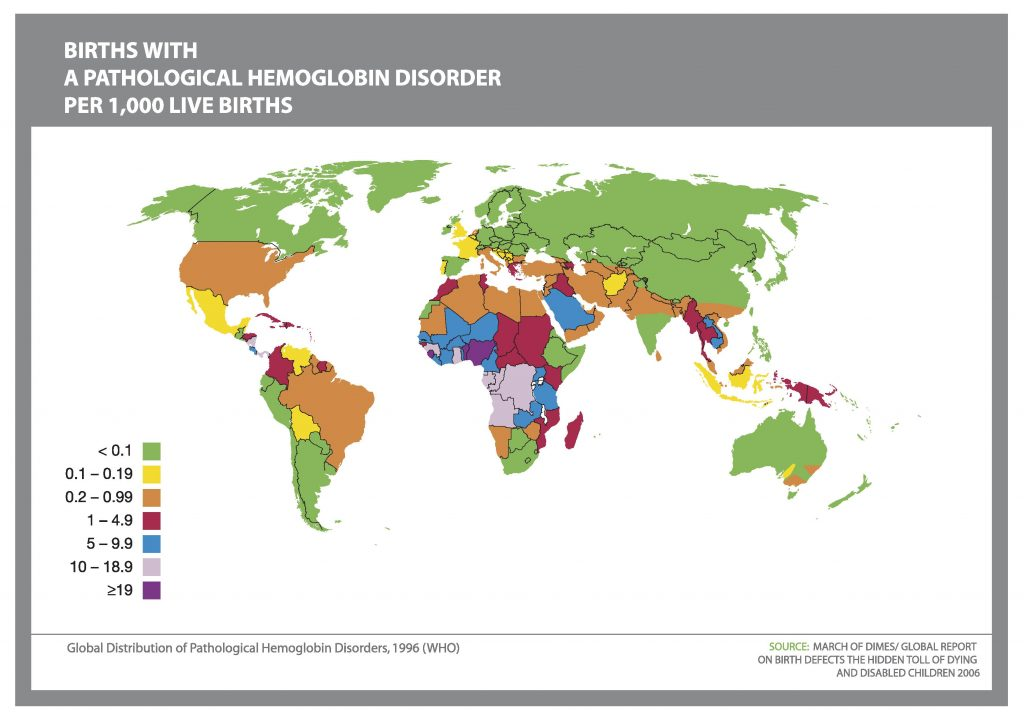
\includegraphics[width= 1\textwidth, height=1\textheight, keepaspectratio]{img/World-map-TIF-1024x724.jpg}
\caption{Immagine reperita sul sito del Thalassemia International Federation} \label{TIF}
\end{center}
\end{figure}

\subsubsection{Tipologie di Talassemia}
La alterata sintesi della catena $\beta$ - che causa le $\beta$-talassemie - può verificarsi durante la fase di trascrizione, formazione o traslocazione dell'mRNA, più di preciso sul cromosoma 11\cite{atzeni2002beta}. 
Le caratteristiche cliniche della $\beta$-talassemia variano a seconda del quadro sintomatico, la gravità della patologia varia tra due estremi,  l'essere un portatore ``sano'' o essere un malato grave della così detta ``Anemia Mediterranea''. Vengono elencate le tipologie di talassemia:

\begin{enumerate}
\item \subsubsection{Talassemia minor o microcitemia} Indica la situazione asintomatica dell'anomalia genetica. Ciò comporta alterazioni caratteristiche dei globuli rossi che risultano più piccoli e più pallidi rispetto a quelli normali.
Spesso ne consegue una condizione anemica più o meno accentuata (Anemia microcitica).
\item \subsubsection{Talassemia intermedia} Indica il quadro clinico meno grave di quello major in quanto per lo stato anemico non è generalmente necessaria una terapia trasfusionale, talvolta alcune persone con talassemia intermedia intraprendono la terapia trasfusionale in età più adulta.
\item \subsubsection{Talassemia major o Anemia Mediterranea o Morbo di Cooley} 
Indica un quadro clinico molto grave e rapidamente mortale in assenza di cure. Per rimediare alla carenza di emoglobina e alla notevole anemia, i talassemici necessitano fin dai primi mesi di vita, di una regolare terapia trasfusionale con intervalli di 10-20 giorni in media\cite{talassemicipiemonte}. 
\end{enumerate}

\subsection{Diagnosi}
La maggior parte delle persone vengono a conoscenza accidentalmente del loro stato patologico, quando l'emocromo mostra una lieve anemia microcitica, il che è una condizione necessaria ma non sufficiente per diagnosticare la talassemia, in quanto l'anemia potrebbe essere data da altre cause. Per accertarsi della diagnosi è necessario controllare il volume cellulare medio (MCV) e l'ampiezza di distribuzione dei globuli rossi (RDW)\cite{muncie2009alpha}.

Generalmente la diagnosi di talassemia major o intermedia avviene entro il secondo anno di vita, le caratteristiche più note sono in genere pallore, irritabilità e ritardo di crescita. Le alterazioni scheletriche e facciali tipiche della malattia si manifestano più avanti nel tempo. Nella preadolescenza, si ha un rallentamento della crescita e successivamente possono intervenire complicanze a vari organi o malattie intercorrenti che possono compromettere la qualità di vita dei pazienti e richiedono, ciascuna, specifiche terapie. I pazienti non trattati vanno incontro a morte nell'infanzia o nella prima adolescenza come conseguenza della grave anemia. Uno studio retrospettivo italiano ha dimostrato che se non viene impostata una terapia, la morte in genere avviene nei primi 5 anni di vita \cite{atzeni2002beta}\cite{screening1975}.

\subsection{Terapia}
La terapia standard per le Talassemie consiste nel sottoporre i pazienti a trasfusioni regolari, per mantenere alti i livelli di emoglobina presenti nel sangue. In questo modo è possibile tutelare la circolazione dell'ossigeno nei tessuti e arrestare l'espansione del midollo osseo.

Fare trasfusioni regolari, causa un crescente sovraccarico di ferro nel sangue che porta inevitabilmente a disfunzioni a carico del cuore, del fegato, della milza e dello scheletro \cite{poggi2014studio}. L'accumulo eccessivo di ferro, costringe i talassemici a specifiche terapie quotidiane ``deferrizzanti'', essenziali per mantenersi in buona salute. Solo tramite queste, viene eliminato il ferro in eccesso, che altrimenti, determinerebbe patologie gravi e precoci ai suddetti organi, portando il soggetto alla morte.

\subsection{Malattie derivanti}
La talassemia è una malattia che coinvolge appieno la maggior parte degli organi, avere carenza di emoglobina - il quale compito è trasportare ossigeno a tutti i tessuti del corpo - può creare molteplici disfunzioni e complicanze. 
Uno studio dimostra che la morte di due pazienti su tre è dovuta a malattie derivanti dal malfunzionamento dell'organismo, come: endocrinopatie, epatopatie e cardiopatie, a queste si aggiungono ulteriori rischi infettivi dovuti alle trasfusioni.

\subsubsection{Endocrinopatie}
Le endocrinopatie sono le malattie legate al corretto funzionamento delle ghiandole. Il pancreas, che fa parte del sistema endocrino, è spesso compromesso per via del sovraccarico di ferro e non permette di avere un livello adeguato di secrezione di insulina, portando tra il 40\% e il 55\% dei pazienti al diabete.

\subsubsection{Epatopatia}
L'alterazione del corretto funzionamento della milza - descritto precedentemente - e la possibile presenza di infezioni virali, sono i fattori principali che creano disfunzioni al fegato, uno degli organi più compromessi insieme al cuore. Nel 90\% dei pazienti sopra i 15 anni di età si riscontrano problemi al fegato, una percentuale così alta non può che farne vittima circa il 30\% - 40\%.

\subsubsection{Cardiopatie}
Le disfunzioni cardiache sono la principale causa di decesso per i pazienti talassemici, infatti in passato, quando non venivano effettuate trasfusioni, la degenerazione della massa muscolare cardiaca portava forzatamente alla morte. Attualmente, dove il progesso ha permesso un migliore accesso alle trasfusioni, i decessi per anemie cardiache sono decisamente ridotti, ma è subentrato il danno dovuto agli accumuli di ferro, questo può creare gravi problemi degenerativi alle fibre muscolari, tra queste il cuore.

\subsubsection{Malattie infettive}
Essendo la talassemia una malattia che prevede il trasferimento di sangue, non potevano che insorgere problematiche dovute a malattie contagiose per via parenterale, quali Epatite e HIV.
Con l'introduzione dei trattamenti trasfusionali sono aumentati notevolmente i casi di infezioni, dando origine a numerevoli ``scandali del sangue infetto'' come quello in Sardegna nel dicembre del 2017 che ha contagiato la comunità talassemica sarda dai virus HCV/HIV/HBV \cite{giunti2019etnografia}.


\subsection{Progressi del trattamento trasfusionale}
Dagli anni `50, gli istituti sanitari hanno iniziato a sottoporre i malati a trasfusioni periodiche, questo ha modificato il quadro clinico e la percentuale di sopravvivenza dei malati è aumentata. Non tutti però avevano la possibilità di accedere al trattamento trasfusionale, che avveniva solo in casi di grave anemia, tanto da mettere a rischio la vita del paziente. In quel periodo, sono inoltre state introdotte delle procedure che prevedono la splenectomia - ovvero la rimozione della milza - con lo scopo di ridurre il consumo di sangue e il numero di trasfusioni, e di conseguenza anche il sovraccarico di ferro.\cite{casale2013effect}.

Solo negli anni `60 sono stati introdotti farmaci che permettono la sottrazione dell'eccesso di ferro - accumulatosi in seguito alle ripetute trasfusioni - dall'organismo, con la regolare applicazione di questa terapia, la sopravvivenza dei malati si è fatta progressivamente sempre più lunga\cite{atzeni2002beta}.
Il trattamento ferro-chelante veniva svolto attraverso infusioni sottocutanee di circa dieci ore per almeno cinque giorni a settimana, attualmente vengono rilasciati farmaci ad uso orale che permettono l'eliminazione del ferro per via renale (con le urine) e in parte per via biliare (con le feci).

\section{Assistenza sanitaria su dispositivi mobili}
Il progresso tecnologico rappresenta una delle pietre miliari del ventunesimo secolo, negli ultimi anni gli sviluppi per la comunicazione e il transito di informazioni hanno dato una svolta allo stile di vita e all'erogazione della maggior parte dei servizi. In questo contesto, poter accedere a dei referti in qualsiasi luogo e in qualsiasi momento svolge un ruolo chiave nelle soluzioni sanitarie\cite{SILVA2015265}. 

\subsection{mHealth}
La ``salute mobile'', in inglese mobile health (mHealth) è un termine che definisce l'utilizzo di dispositivi mobili in ambito medico-sanitario, questa è una branca dell'eHealth ``salute digitale'', ovvero la pratica della salute tramite il supporto di strumenti informatici, tecniche di comunicazione medico-paziente e personale specializzato.

L'introduzione dei dispositivi mobili negli anni `90 ha permesso a medici e pazienti di utilizzare - prima tramite i palmari, attualmente tramite tablet e smartphone - prodotti software per l'interscambio di dati sanitari. Ad oggi è di fatto di uso comune utilizzare la tecnologia per svolgere la maggior parte di compiti inerenti alla cura personale, come: gestire cartelle cliniche, visualizzare risultati di laboratorio e allegati medici, richiedere prescrizioni di farmaci e prenotare esami. È inoltre possibile avere un monitoraggio completo della propria salute, per mezzo di wearable e sensori che forniscono risultati e resoconti giornalieri sulla base dei dati raccolti.

Una ricerca \cite{fox2010mobile} del 2012 dà prova che la metà dei possessori di smartphone utilizzava già i propri dispositivi per ottenere informazioni sulla propria salute, ed essendo la percentuale della popolazione che accede a servizi sanitari attraverso telefoni cellulari sempre crescente, attualmente possiamo stimare che un quinto degli utenti esegua operazioni di gestione di dati sanitari tramite applicazioni sul proprio dispositivo.
Lo sviluppo in materia di dematerializzazione di documenti spinge sempre più le autorità sanitarie ad aggiornarsi, creando nuove infrastrutture informatiche che permettano l'accesso e la condivisione di informazioni cliniche e amministrative per via telematica.
In seguito analizziamo le potenzialità e gli svantaggi della sanità digitale.

\subsubsection{Vantaggi della digitalizzazione sanitaria}
Il vantaggio primario consiste nell’agevolazione dello scambio di informazioni medico-paziente, i possibili sviluppi segnerebbero una svolta per le persone impossibilitate - come malati cronici - a recarsi in luoghi che svolgono attività di assistenza sanitaria. La digitalizzazione del suddetto rapporto consentirebbe di eseguire atti medici - che non richiedono la presenza di uno specialista - per mezzo di comunicazione in tempo reale, tali progressi permetterebbero al sistema sanitario di avere a carico meno spese dovute a ricoveri e operazioni di gestione di cartelle cliniche e archivi cartacei, rendendone inoltre la consultazione immediata.

\subsubsection{Problematiche della digitalizzazione sanitaria}
Le problematiche legate alla digitalizzazione sanitaria riguardano principalmente le misure di sicurezza dei dati. Sono necessarie tecniche che rendano le informazioni: disponibili, consultabili in qualsiasi momento, confidenziali, riservate - ad un gruppo limitato di persone, quali medico e paziente - e integre.
Non sono da meno problematiche derivanti dall'utilizzo stesso della tecnologia, che ancora oggi, mettono in difficoltà pazienti anziani che necessitano di maggiore supporto per fruire in modo corretto dei servizi.

\subsection{Retroscena di applicazioni mobili orientati alla Talassemia}
In questo paragrafo viene discusso il funzionamento di due applicazioni orientate alla talassemia, ne viene studiato il comportamento e le modalità con la quale rispondono alle necessità dei pazienti.

\subsubsection{THALIA Mobile App}
Sviluppatori-pazienti affetti da emoglobinopatie hanno creato THALIA App [Fig. \ref{thaliaA}], definita come ``L'assistente digitale esperto di persone con talassemia e anemia falciforme''. 
THALIA Mobile App è stata sviluppata nel programma quadriennale di attività - che va dal 2018 al 2021 - del TIF ``Thalassemia in Action'' (THALIA) ed è co-finanziata dal Terzo Programma Salute dell'Unione Europea.
L'applicazione ha come scopo principale fornire un ausilio per la gestione della propria malattia. Il fulcro è il calendario [Fig. \ref{thaliaB}] che permette di memorizzare dati riguardanti trasfusioni ed esami passati e futuri, inoltre l'applicazione fornisce un vasto accesso a informazioni sanitarie molto specifiche riguardanti le emoglobinopatie, sia in termini scientifici, sia in materiale educativo [Fig. \ref{thaliaC}] pubblicato dalla Thalassemia International Federation \cite{tahliaapp}.

\begin{figure}[H]
\centering
\subfloat[][\emph{Splash screen}]
{
\includegraphics[width=.2\textwidth]{img/THALIA App/THALIA (2).jpg} \label{thaliaA}} \quad
\subfloat[][\emph{Calendario con eventi}]
{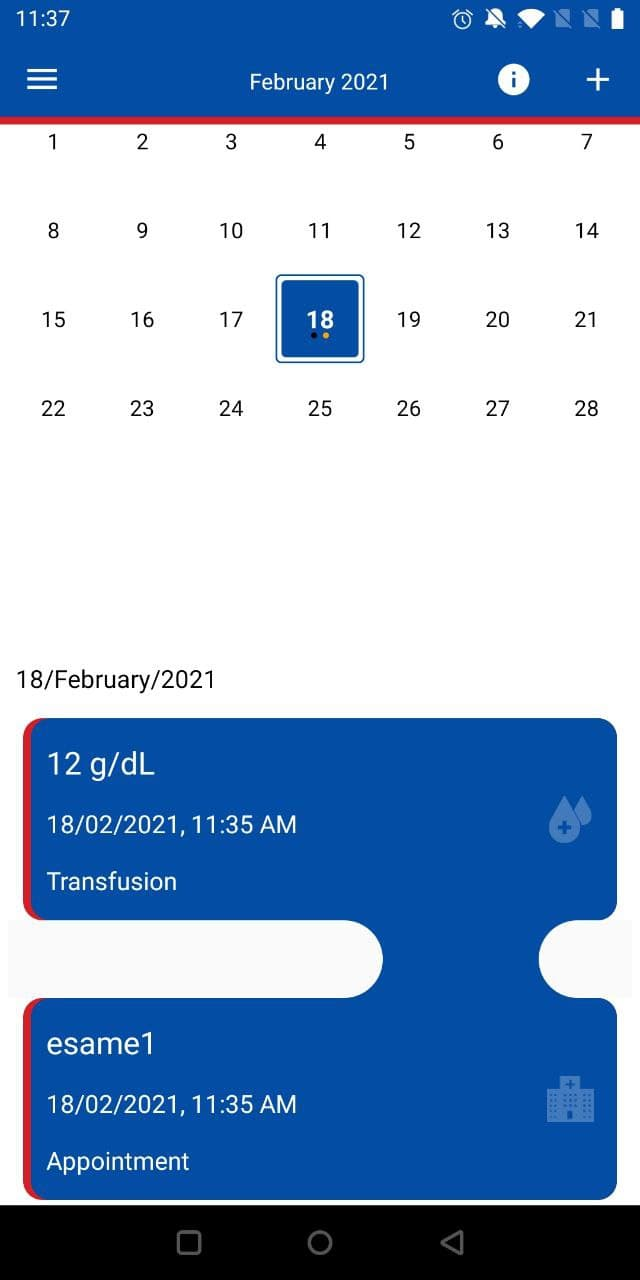
\includegraphics[width=.2\textwidth]{img/THALIA App/THALIA (1).jpg} \label{thaliaB}} \quad
\subfloat[][\emph{Menu laterale}]
{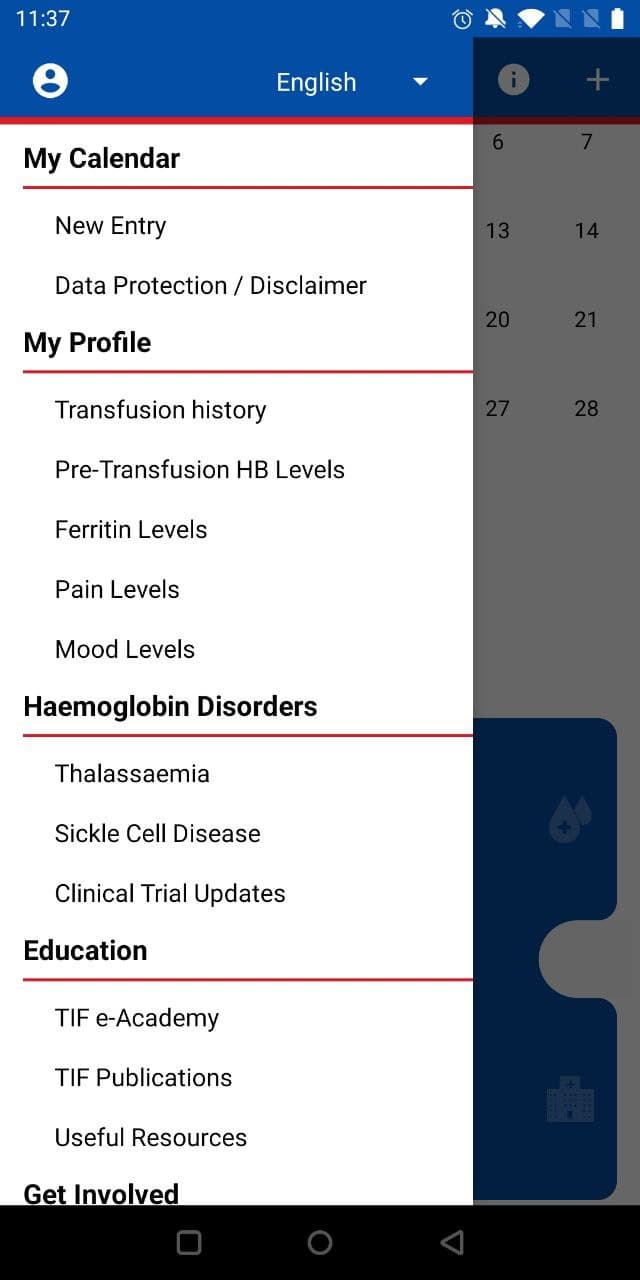
\includegraphics[width=.2\textwidth]{img/THALIA App/THALIA (3).jpg} \label{thaliaC}} \quad
\caption{Screenshot dell'applicazione THALIA Mobile App}
\label{thaliaD}
\end{figure}

\textbf{Punti di forza:}
\begin{itemize}
    \item Semplicità di utilizzo: aggiungere, rimuovere, modificare e visualizzare gli eventi nel calendario.
    \item Possibilità di aggiungere le trasfusioni passate in un calendario esterno all'applicazione in questione
    \item Supporto da parte della Federazione Internazionale Talassemici
    \item Fonte di informazioni attendibili e aggiornate
    \item Possibilità di condividere i propri dati clinici con i medici
    \item Monitoraggio e controllo dello stato del paziente: come eventuali sintomi, umore e fatica
\end{itemize}

\textbf{Debolezze:}
\begin{itemize}
    \item Nessun controllo degli accessi
    \item Supporto fornito in un periodo limitato: essendo un progetto quadriennale c'è il rischio che dopo il tempo predefinito il progetto venga ``messo da parte''
    \item Impossibilità di programmare trasfusione future
    \item Assenza di una sezione dedicata alle terapie
    \item Design confusionario
\end{itemize}

\subsubsection{ThaliMe}
ThaliMe è un'applicazione creata ad hoc per la comunità talassemica, il suo scopo è interconnettere tramite un social network tutti i diretti interessati alla patologia, non solo pazienti, ma anche medici, operatori sanitari e familiari. L'assistenza sanitaria si basa sulla condivisione di informazioni che vengono aggiunte dal paziente e visualizzate dai medici, fornendogli una partecipazione diretta alla cartella clinica del malato.
Come la maggior parte dei social network, l'app permette uno scambio di messaggi tra ``amici'' aggiunti alla propria cerchia (fig. \ref{thalimeB}) e una personalizzazione del proprio profilo pubblico.
\`E presente una sezione (fig. \ref{thalimeC}) dedicata al controllo di svariate patologie - cardiopatie, epatopatie, malattie del sangue, etc - legate alle emoglobinopatie che permette di registrare dati clinici strettamente legati agli organi in questione \cite{mcmicking2018thalime}.

\begin{figure}[]
\centering
\subfloat[][\emph{Home con le news}]
{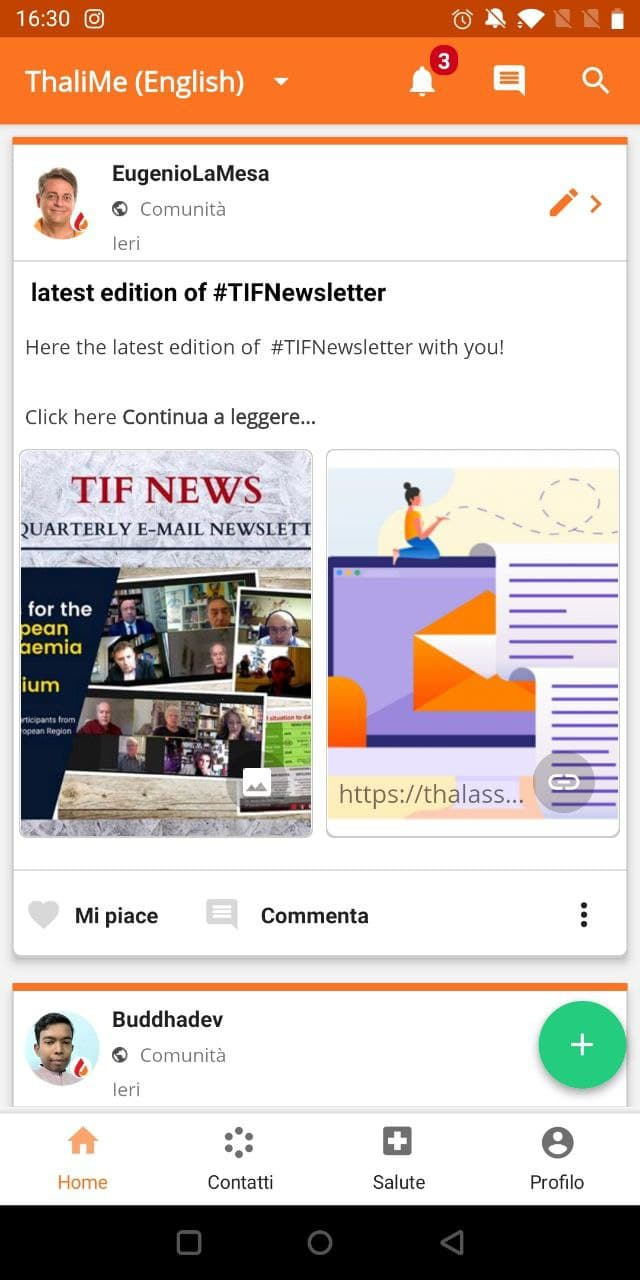
\includegraphics[width=.2\textwidth]{img/ThaliMe/ThaliMe (4).jpg} \label{thalimeA}} \quad
\subfloat[][\emph{Community nelle vicinanze}]
{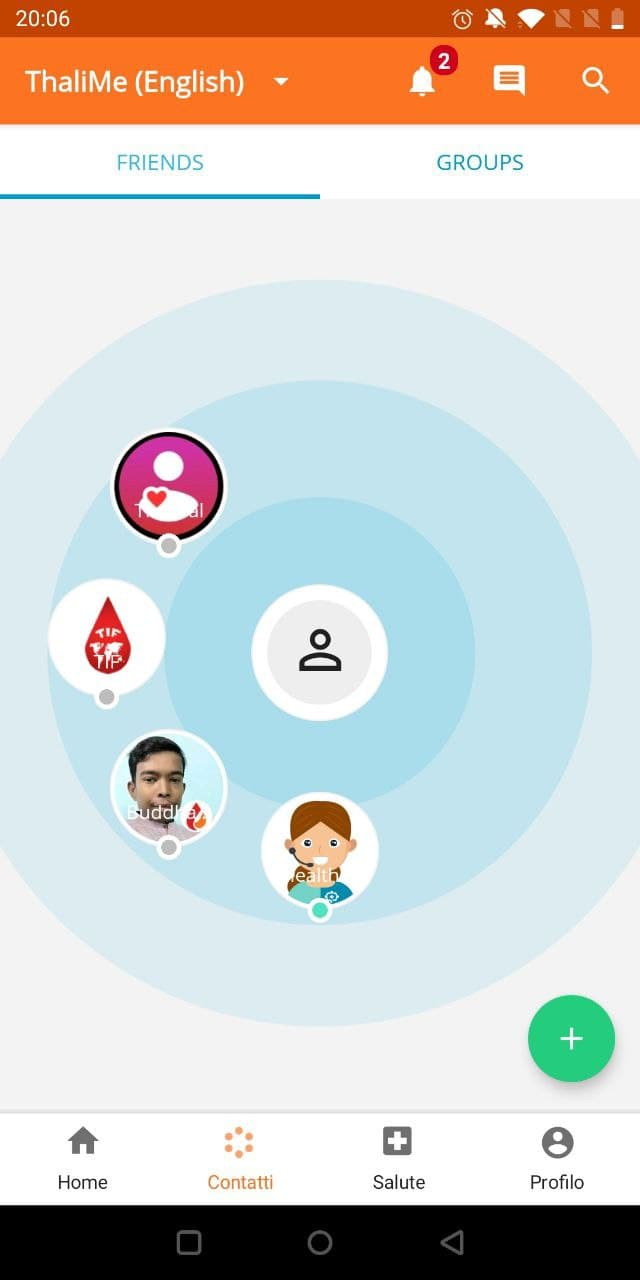
\includegraphics[width=.2\textwidth]{img/ThaliMe/ThaliMe (1).jpg} \label{thalimeB}} \quad
\subfloat[][\emph{Diario delle informazioni sanitarie}]
{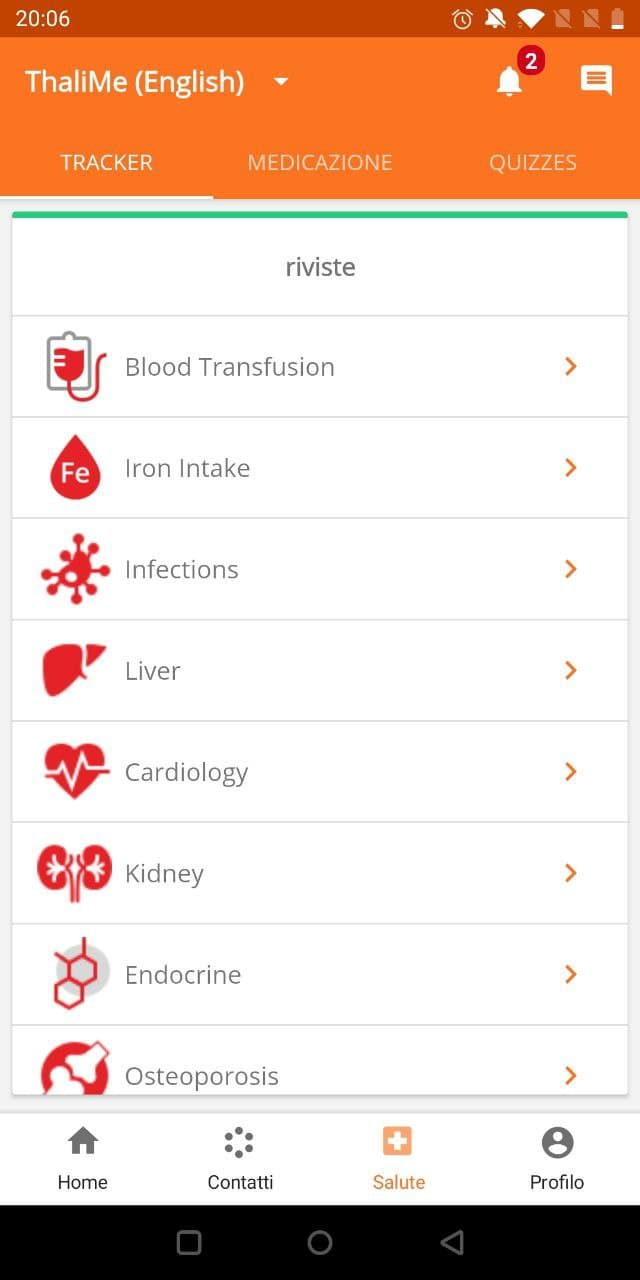
\includegraphics[width=.2\textwidth]{img/ThaliMe/ThaliMe (5).jpg} \label{thalimeC}} \quad
\subfloat[][\emph{Profilo personale}]
{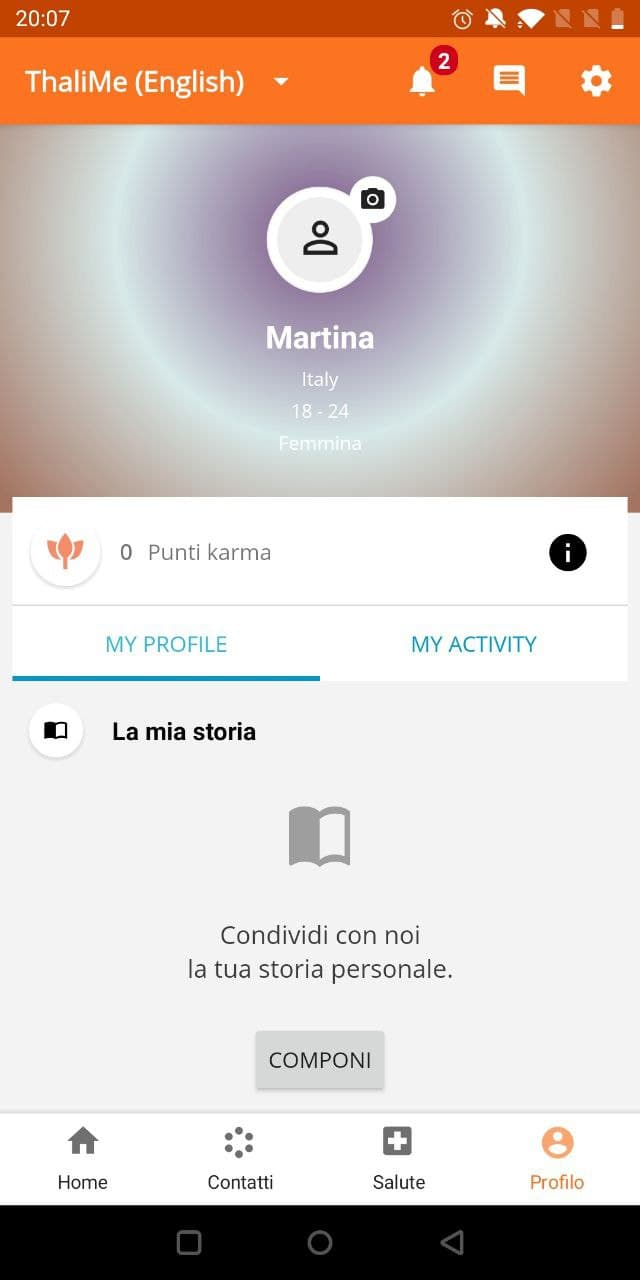
\includegraphics[width=.2\textwidth]{img/ThaliMe/ThaliMe (2).jpg} \label{thalimeD}} \quad
\caption{Screenshot dell'applicazione ThaliMe}
\label{thalimeE}
\end{figure}

\textbf{Punti di forza:}
\begin{itemize}
    \item Possibilità di socializzare con persone della propria comunità
    \item Contatto diretto con personale medico specializzato
    \item Controllo degli accessi ai dati riservati
    \item Fonte di informazioni attendibili e aggiornate
    \item Condivisione dei propri dati clinici con il personale medico in modo diretto
    \item Controllo su tendenze anomale dei dati personali
    \item Monitoraggio e controllo dello stato del paziente: come eventuali sintomi, umore e fatica
\end{itemize}

\textbf{Debolezze:}
\begin{itemize}
    \item Assenza di una schermata che mostra eventi futuri su un calendario
    \item Supporto fornito in un periodo limitato: essendo un progetto quadriennale c'è il rischio che dopo il tempo predefinito il progetto venga messo da parte
    \item Limitato in assenza di connessione internet 
\end{itemize}


\subsection{Necessità dei pazienti affetti da talassemia}
Sviluppare un prodotto software fruibile prevede lo studio delle necessità degli utenti che ne faranno utilizzo, a tal proposito sono stati contattati medici dell'ospedale Sant'Anna di Cona (FE) specializzati in talassemia, è stato presente in particolar modo il supporto della Dott.ssa Maria Rita Gamberini - direttrice del Day Hospital della Talassemia e delle Emoglobinopatie - e della Dott.sa Mari Elisa - dirigente medico in medicina interna. 
In seguito all'incontro sono state valutate le difficoltà e le necessità dei pazienti affetti da emoglobinopatie.

Innanzitutto è necessario che il paziente rispetti controlli periodici, appuntamenti per la terapia trasfusionale e l'assunzione adeguata di farmaci.A tal fine diventa essenziale avere uno spazio dove tenere traccia di ogni informazione ritenuta utile, una cronologia per visionare gli eventi passati e un calendario per segnalare eventi futuri riguardanti le tre categorie. 

D'altronde essendo i soggetti sottoposti molteplici controlli e visite di routine, avere un quadro completo degli esami passati, risultati annessi, faciliterebbe significativamente la gestione della propria cartella clinica, pertanto si esigono dei promemoria a lungo termine per eventi futuri.
Le dimenticanze del paziente sono spesso causa di grandi disagi perché è proprio a causa di queste che le terapie non vengono seguite nel modo adatto, diventa quindi essenziale strutturare un programma di notifiche che faccia da supporto. 

\subsection{Motivazioni}
I pazienti $\beta$-talassemici in Italia sono circa 7 mila, di cui meno del 10\% ha più di quarant'anni, la maggior parte prende nota dei propri dati clinici attraverso un dispositivo mobile, sia usando strumenti innovativi forniti dalle autorità sanitarie (p.e. Fascicolo sanitario), sia usando applicazioni di terze parti, che hanno sicuramente modo di soddisfare le richieste dell'utente - come aggiungere sveglie o promemoria - ma non sono capaci di fornire un ``quadro completo'' del paziente talassemico. 

In un mondo che sta entrando sempre più nell'era della digitalizzazione, risulta necessario creare dei prodotti software che possano dare ausilio ai pazienti, in particolar modo a quelli affetti da talassemia, costretti a seguire un regime stretto di terapie, analisi e controlli. 
L'esigenza di un'agenda digitale per dispositivi mobili emerge nella comunità talassemica italiana, dal momento in cui non sono presenti prodotti software abbastanza soddisfacenti da consentirne l'uso giornaliero. 

In seguito all'analisi del paragrafo 1.2.2 si può desumere l'inadeguatezza delle app analizzate nel supporto dell'intera comunità. Si tratta di prodotti che non accolgono la lingua italiana, hanno un design e delle funzionalità troppo scarne o troppo elaborate da permetterne la comprensione all'utente poco pratico, inoltre, è poco presente il supporto fornito dai produttori, tali motivazioni ne giustificano il disuso. 


\chapter{TalApp}

\section{Obiettivi e requisiti}
Per mezzo della documentazione raccolta nel paragrafo 1.2.3, è stato possibile stilare una lista di obiettivi e requisiti per progettare e sviluppare un'applicazione Android per la gestione di dati clinici orientati alla Talassemia.

\subsection{Obiettivo primario:} 
Sviluppare e valutare la fattibilità di uno strumento per migliorare i rapporti tra la raccolta dei risultati e la salute dei pazienti affetti da talassemia. 

Elenco delle funzionalità primarie:

\begin{enumerate}
    \item Creare un'applicazione che permetta di gestire una ``cartella clinica'' per le persone affette da talassemia.
    \item Avere la possibilità di memorizzare in un unico luogo virtuale gli appuntamenti e visite da svolgere in futuro e tenere una cronologia di quelli passati, questo implica:
    \begin{itemize}
        \item La necessità di poter effettuare un login, trattandosi di dati sensibili
        \item La possibilità di aggiungere, modificare ed eliminare eventi (quali visite ed esiti)
        \item Visualizzazione di tali eventi in un calendario
    \end{itemize}
    \item Impostare degli allarmi e notifiche che permettano di avvisare in anticipo il paziente dei prossimi eventi futuri, tipi di avvisi:
    \begin{itemize}
        \item Prossima trasfusione da fare
        \item Prossimi esami da fare
        \item Assuzione di medicinali
    \end{itemize}
\end{enumerate}

\subsection{Requisiti funzionali}
\begin{enumerate}
    \item Operazioni di login:
    \begin{itemize}
        \item Quando l'utente apre l'applicazione deve aver la possibilità di registrarsi o accedere per poter gestire i propri dati
        \item L'utente deve avere la possibilità di iscriversi con una mail personale generica valida oppure un account Google pre esistente
        \item L'utente deve avere la possibilità di resettare la propria password in caso di dimenticanza
    \end{itemize}
    \item Operazioni della home:
    \begin{itemize}
        \item L'utente deve poter accedere alle aree riguardanti il calendario, le trasfusioni, gli esami e le terapie
    \end{itemize}
    \item Operazioni del calendario:
    \begin{itemize}
        \item L'utente deve poter aggiungere appuntamenti per trasfusioni, esami o aggiungere nuove terapie
        \item L'utente deve poter visualizzare gli eventi di un singolo giorno selezionando la data sul calendario
    \end{itemize}
    \item Operazioni di inserimento per una nuova trasfusione:
    \begin{itemize}
        \item L'utente deve poter aggiungere data e ora della prossima trasfusione
        \item L'utente, se ne è a conoscenza, deve poter indicare il numero di unità di sangue da ricevere durante la terapia trasfusionale
        \item L'utente deve poter scrivere nuove eventuali note a riguardo
    \end{itemize}
    \item Operazioni di inserimento per un nuovo esame
    \begin{itemize}
        \item L'utente deve poter inserire la data e l'ora del prossimo esame, se questo ha una periodicità nel tempo (es: ogni 6 mesi, ogni anno, etc..)
        \item Il tipo di esame da svolgere, se di laboratorio o strumentale
        \item In base al tipo di esame deve poter assegnargli un nome avendo dei suggerimenti da una lista, deve anche poter aggiungere nuovi nomi per esami non in lista
        \item Deve poter esprimere se deve essere a digiuno per quell'esame o meno
        \item Deve poter esprimere se deve fare un trattamento anticipato, e aggiungere il tipo di trattamento usando uno spazio per scrivere (ad esempio se deve interrompere una terapia o deve fare una raccolta specifica)
        \item L'utente deve poter scrivere nuove eventuali note a riguardo
    \end{itemize}
    \item Operazioni di inserimento per una nuova terapia
    \begin{itemize}
        \item L'utente deve poter inserire la data di inizio di una nuova terapia
        \item L'utente deve poter indicare se la terapia è momentanea oppure è periodica e quindi si ripete nel tempo
        \item L'utente deve poter impostare la data di fine della terapia se questa è periodica
        \item L'utente deve poter salvare il nome del farmaco e il relativo dosaggio
        \item L'utente deve poter attivare delle notifiche per ricordargli di prendere il farmaco
        \item L'utente deve avere la possibilità di impostare nessuna, una o più sveglie per del farmaco in questione
        \item L'utente deve poter scrivere nuove eventuali note a riguardo
    \end{itemize}
    \item Operazioni riguardanti le trasfusioni:
    \begin{itemize}
        \item L'utente deve poter velocemente vedere quando è stata svolta l'ultima trasfusione e quando sarà la prossima
        \item L'utente deve poter visualizzare quanto tempo è passato tra l'ultima trasfusione e il giorno attuale
        \item L'utente deve poter aggiungere dati riguardanti l'ultima trasfusione svolta, se già presenti, viene data la possibilità di modificarli
        \begin{itemize}
        \item L'utente deve poter aggiungere il valore dell'emoglobina registrata nel giorno in cui viene svolta la terapia trasfusionale
        \item L'utente deve poter modificare le note e l'unità di sangue acquisita, se queste erano già state segnalata, altrimenti può o aggiungerle
        \item L'utente deve poter eliminare l'ultima trasfusione svolta
        \end{itemize}
        \item L'utente deve poter visualizzare lo storico delle trasfusioni effettuate fino ad oggi
        \begin{itemize}
        \item L'utente deve poter fare una ricerca tra i promemoria delle trasfusioni passate
        \item L'utente deve poter modificare i valori delle trasfusioni passate o eliminarle
        \end{itemize}
        \item L'utente deve poter vedere un grafico che mostra l'andamento del valore dell'emoglobina in ogni trasfusione precedente (nell'ultimo anno)
        \end{itemize}
        \item Operazioni riguardanti gli esami:
        \begin{itemize}
        \item L'utente deve poter distinguere gli esami di laboratorio e gli esami strumentali
        \item L'utente deve poter visualizzare i prossimi esami da svolgere in modo veloce e intuitivo
        \item L'utente deve poter aggiungere dati all'ultimo esame svolto
        \begin{itemize}
        \item L'utente deve poter memorizzare un allegato dell'esame
        \item L'utente deve poter memorizzare un esito dell'esame
        \item L'utente deve poter modificare la periodicità dell'esame e le note inerenti
        \end{itemize}
        \item L'utente deve poter visualizzare la cronologia degli esami passati
        \begin{itemize}
        \item L'utente deve poter fare una ricerca tra i promemoria degli esami passati
        \item L'utente deve poter modificare i valori degli esami passati o eliminarli
        \end{itemize}
    \end{itemize}
    \item Operazioni riguardanti le terapie:
    \begin{itemize}
        \item L'utente deve poter visualizzare velocemente le terapie attuali e le relative informazioni
        \item L'utente deve poter visualizzare la cronologia delle terapie passate
        \item L'utente deve poter modificare o eliminare le terapie attuali
    \begin{itemize}
    \item L'utente deve poter modificare la periodicità della terapia
    \item L'utente deve poter modificare la data di fine terapia
    \item L'utente deve poter modificare il dosaggio
    \item L'utente deve poter attivare o disattivare le notifiche per la data terapia
    \item L'utente deve poter modificare, aggiungere o eliminare le sveglie inerenti a quella terapia
    \item L'utente deve poter interrompere la terapia
    \end{itemize}
    \item L'utente deve poter visualizzare la cronologia delle terapie passate
    \begin{itemize}
    \item L'utente deve poter fare una ricerca tra i promemoria delle terapie passate
    \item L'utente deve poter modificare i valori delle terapie passate o eliminarle
    \end{itemize}
    \end{itemize}
    \item Operazioni riguardanti le impostazioni:
    \begin{itemize}
    \item L'utente può decidere se attivare o meno le notifiche per la prossima trasfusione
    \item L'utente può decidere quando ricevere la notifica, se attiva, per la prossima trasfusione
    \item L'utente può decidere se attivare o meno le notifiche per gli esami strumentali
    \item L'utente può decidere quando ricevere la notifica, se attiva, per gli esami strumentali
    \item L'utente può decidere se attivare o meno le notifiche per gli esami di laboratorio
    \item L'utente può decidere quando ricevere la notifica, se attiva, per gli esami di laboratorio
    \item L'utente deve poter effettuare il logout
    \end{itemize}
\end{enumerate}

\subsection{Requisiti non funzionali}
\begin{enumerate}
\item Il sistema per funzionare deve potersi collegare ad un database esterno per accedere al database
\item Se il sistema non riesce a collegarsi alla rete esterna deve poterlo notificare all'utente
\item Operazioni della home:
\begin{itemize}
\item Quando il login viene effettuato correttamente allora deve essere visualizzata la home
\item La home deve fornire dati riguardanti le ultime operazioni volte (quali trasfusioni, esami e terapie)
\item La home deve essere disponibile in meno di un secondo
\item La home deve essere caratterizzata da elementi e colori che permettano una navigazione semplice tra le varie schermate
\end{itemize}
\item Operazioni del calendario:
\begin{itemize}
\item Il calendario deve poter visualizzare quali eventi sono salvati in ogni giorno del mese corrente
\item Il calendario deve poter mostrare anche i mesi precedenti e successivi a quello attuale
\item Nella scheda del calendario deve esserci la possibilità di ricerca globale tra tutti i dati
\item Toccando su un singolo giorno del calendario deve esserci la possibilità di visualizzare gli eventi relativi a tale giorno
\end{itemize}
\item Operazione di gestione degli eventi:
\begin{itemize}
\item Il sistema deve poter salvare in un database esterno nuovi eventi, come trasfusioni, esami e terapie con i relativi dati inseriti dall'utente
\item Il sistema deve poter fornire un resoconto dei dati specifici dell'evento specifico
\item Il sistema deve poter fornire una cronologia o lista (in ordine cronologico) degli eventi passati di quella specifica categoria
\end{itemize}
\item Operazioni di notifica:
\begin{itemize}
\item Il sistema deve poter notificare correttamente le sveglie impostate dall'utente per le singole terapie, ove esistenti
\item Il sistema deve poter inviare delle notifiche per i prossimi esami o trasfusioni da effettuare, in base alle preferenze dell'utente
\item Il sistema deve poter distinguere le notifiche degli esami di laboratorio o strumentali
\end{itemize}
\end{enumerate}

\section{Entità e casi d'uso}
Per poter creare funzionalità soddisfacenti per i requisiti posti, esige studiare delle componenti che ne permettano l'implementazione, solo in seguito verranno illustrati i diagrammi UML e le principali attività.

Di seguito un elenco degli attori principali che saranno protagonisti nei possibili casi d'uso:

\begin{itemize}
    \item \subsubsection{Utente}
    L'utente è una persona generica che intende utilizzare l'elaborato software, per lo scopo di questo progetto, è indicato che l'utente che fa uso dell'applicazione sia una persona affetta da talassemia che intende visualizzare e gestire i propri dati clinici.
    
    \item \subsubsection{Autenticazione Firebase}
    Firebase Authentication è un SDK - (Software Development Kit) in italiano "pacchetti di sviluppo per applicazioni" - che permette l'autenticazione degli account. Tramite le sue funzionalità di backend (invisibili all'utente) si certifica l'identità degli utenti, utilizzando mail e password, oppure provider di identità federati, come: Google, Facebook, Twitter, etc \cite{firebaseAuth}.

    \item \subsubsection{Storage per Firebase}
    Storage è un servizio di archiviazione affiliato a Firebase, l'SDK permette il caricamento in rete di file audio, video e contenuti di altro tipo. \`E supportato da protocolli di sicurezza e connettività gestiti da Google \cite{firebaseStorage}.
    
    \item \subsubsection{Cloud Firestore }
    Cloud Firestore, come i precedenti, appartiene alle librerie Firebase ed è un database la sua funzione principale è raccogliere dati personali degli utenti.  Si analizza la struttura del database utilizzato e i suoi compiti nel capitolo successivo.  
\end{itemize}

\subsection{Diagrammi UML}
Nei diagrammi UML \ref{2.1} e \ref{2.2} si espongono i casi d'uso che descrivono il la relazione sistema-utente.

\begin{figure}[h]
\begin{center}
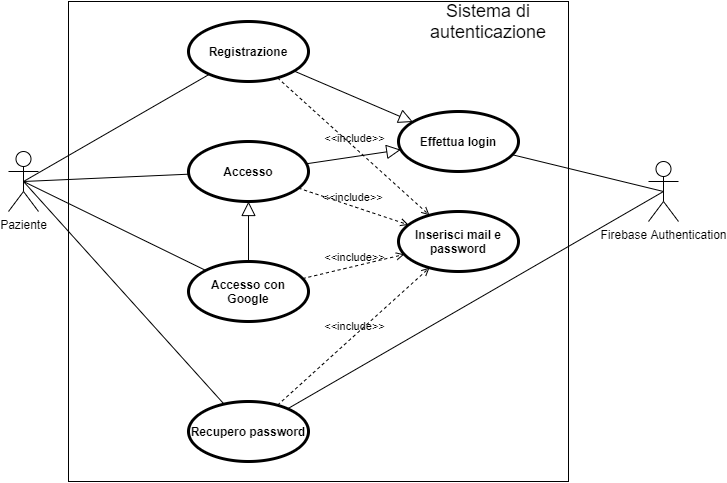
\includegraphics[width= 1\textwidth, height=1\textheight, keepaspectratio]{img/Diagrammi/Diagrammi-Autenticazione.png}
\caption{Diagramma UML del caso d'uso in fase di autenticazione} \label{2.1}
\end{center}
\end{figure}

La figura \ref{2.1} descrive l'autenticazione, una fase iniziale e obbligatoria, alla quale il paziente deve sottoporsi. Certificare l'identità è una procedura chiave per garantire sicurezza dei dati clinici dell'utente; in assenza di riconoscimento non vi è possibilità di usufruire dei servizi di TalApp.

Le possibili operazioni che l'utente può svolgere sono: 
\begin{enumerate}
    \item Accesso: nel caso in cui l'utente sia già iscritto può effettuare l'accesso direttamente inserendo mail e password.
    \item Registrazione: nel caso in cui l'utente sia non è iscritto, può registrarsi inserendo una mail e una password, queste diventeranno poi le credenziali d'accesso.
    \item Accesso con Google: per certificarsi con questa funzionalità si esige che l'utente possieda un account Google, sia la registrazione che il login possono essere effettuati tramite questa componente.
    \item Recupero password: nel caso in cui l'utente sia registrato ma non ricorda le credenziali d'accesso al servizio, può recuperarle inserendo la mail utilizzata per registrarsi. Firebase Authentication invia una messaggio alla mail inserita con un link tramite il quale viene avviata la procedura di reimpostazione della password.
\end{enumerate}


\begin{figure}[h] 
\begin{center}

\includegraphics[width= 1.1\textwidth, height=1\textheight, keepaspectratio]{img/Diagrammi/Diagrammi-TalApp.png}
\caption{Diagramma UML del caso d'uso corpo dell'applicazione} \label{2.2}
\end{center}
\end{figure}

La figura \ref{2.2} mostra una situazione più complessa rispetto alla precedente, gli attori aumentano di numero e viene introdotto nello schema Cloud Firestore, il quale svolge delle mansioni influenti nell'ambiente raffigurato, quale aggiornare il database online ogni qualvolta avviene una modifica della cartella clinica.

Le possibili operazioni che l'utente può svolgere sono: 

\begin{enumerate}
    \item Visualizzazione del calendario: osservare eventi inseriti passati e futuri, distinguendo trasfusioni, un esami o una terapie. Se interessato a consultare gli eventi di una singola giornata, viene stilata una lista degli eventi del periodo di riferimento. 
    \item Aggiunta di una trasfusione, esame o terapia: inserimento di rapporti nella cartella clinica, variano a seconda della tipologia dell'evento che si vuole inserire.  
    \item Modifica delle impostazioni: aggiornamento delle impostazioni, scelta di attivazione di notifiche inerenti ad eventi futuri. Possibilità di effettuare il logout dall'applicazione, Firebase Authentication si occupa di scollegare l'account dall'istanza dell'applicazione sul dispositivo in uso.
    \item Eliminazione o modifica di un evento: la modifica comprende l'inserimento di nuovi dati, questi variano in base alla tipologia dell'evento. Modificando un esame, viene introdotta la gestione degli allegati, quali inserimento, modifica e rimozione, Firestore Storage memorizza eventuali variazioni di immagini nella raccolta.
\end{enumerate}

\section{Schermate e funzionalità}
\subsection{Mockup}
In fase di progettazione è stato creato un mockup adeguato che permettesse l'inclusione delle funzionalità redatte nei requisiti. Le grafiche si basano su layout semplici, ampi bottoni material design e suddivisione dell’albero di navigazione per colori, facilitando all’utente l’orientamento tra le funzionalità. Ogni evento ha un colore di riferimento: rosso per le trasfusioni, blu per gli esami e verde per le terapie. La dimensione del font è grande e ben leggibile e le schermate non hanno un eccesso di contenuti, in figura \ref{2.3} alcuni estratti dal mockup iniziale.

\begin{figure}[H]
\centering
\subfloat[][\emph{Accesso}]
{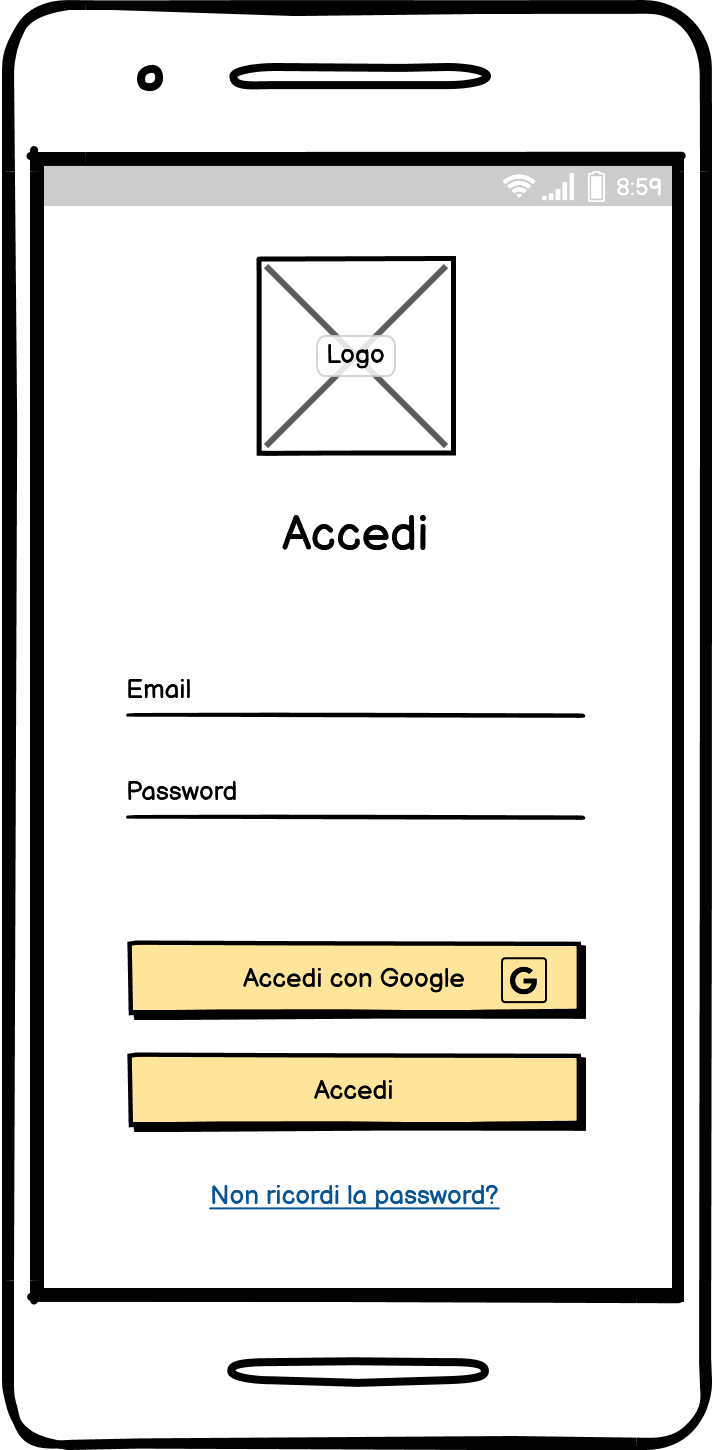
\includegraphics[width=.2\textwidth]{img/Mockup/Accedi.png} \label{2.3a}} \quad
\subfloat[][\emph{Home}]
{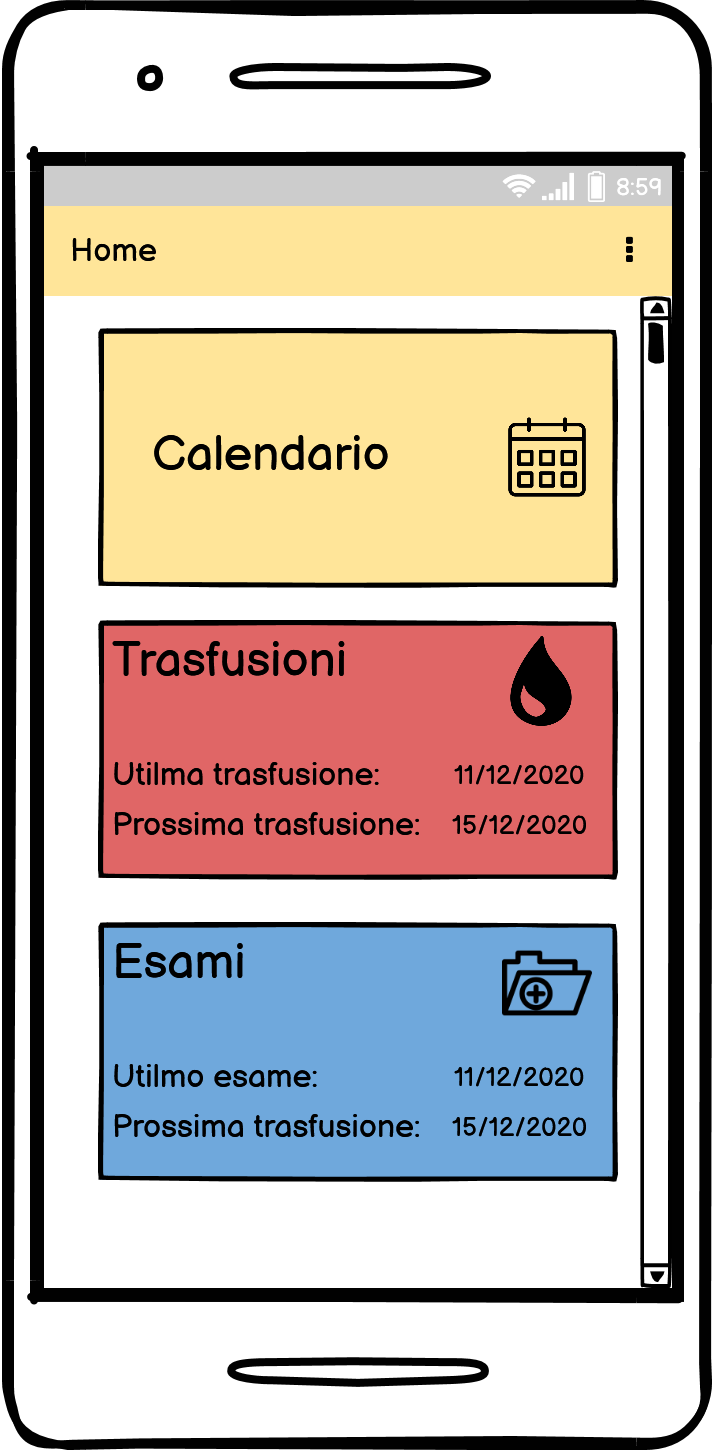
\includegraphics[width=.2\textwidth]{img/Mockup/Home 1.png} \label{2.3b}} \quad
\subfloat[][\emph{Calendaro}]
{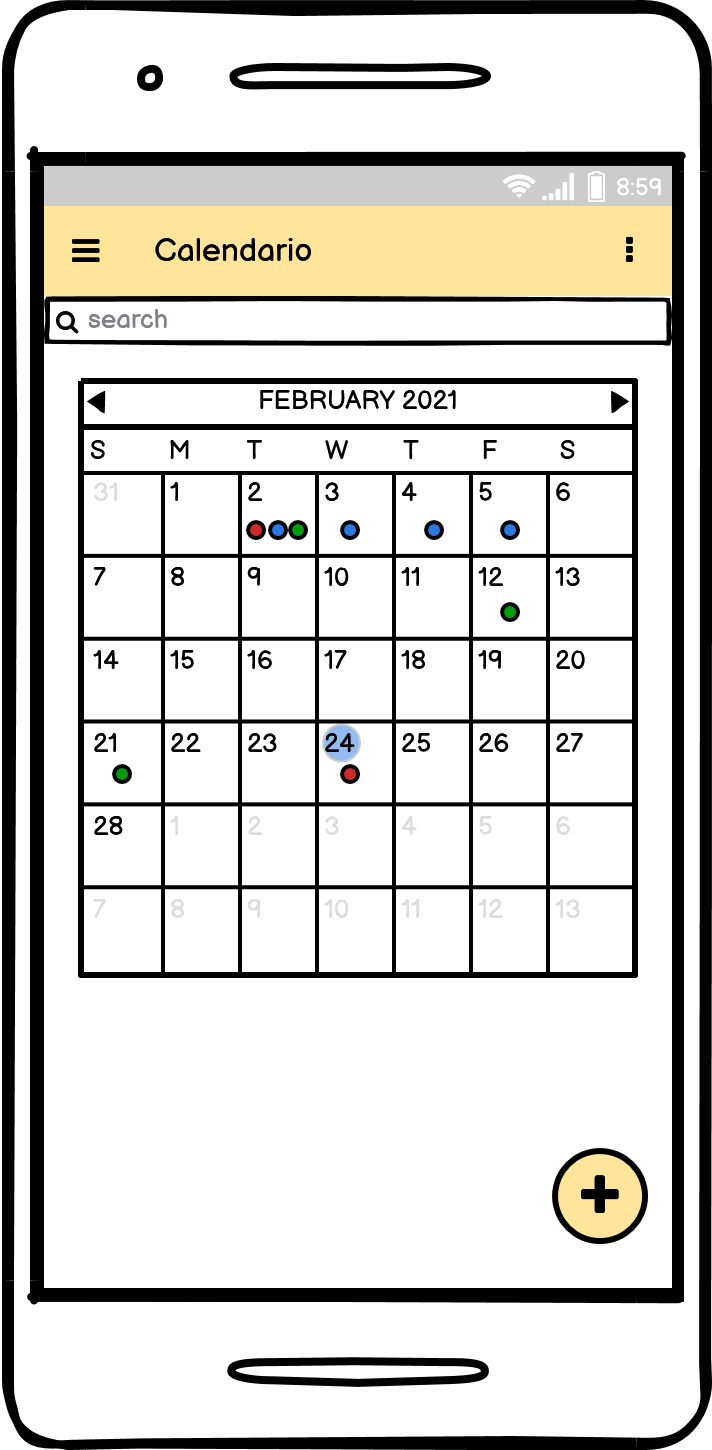
\includegraphics[width=.2\textwidth]{img/Mockup/Calendario 1.png} \label{2.4c}} \quad
\subfloat[][\emph{Trasfusioni}]
{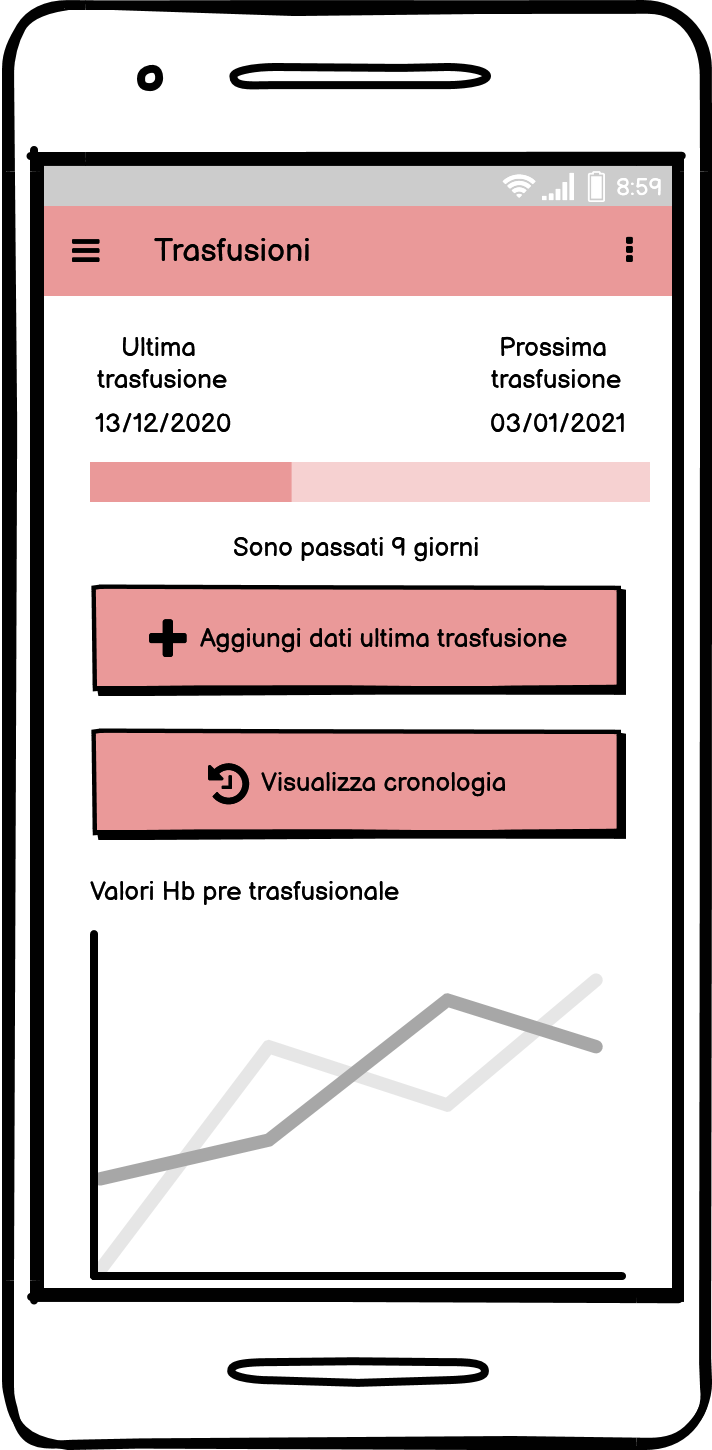
\includegraphics[width=.2\textwidth]{img/Mockup/Trasfusioni.png} \label{2.3d}} \quad
\caption{Mockup iniziale}
\label{2.3}
\end{figure}

\subsection{Accesso e registrazione}
In questo paragrafo si presentano schermate che consentono l'accesso alla cartella clinica.
Come illustrato nel caso d'uso in figura \ref{2.1}, il paziente necessita di compiere azioni diverse, in base alla sua presenza nel database degli accessi, memorizzato da Firebase Authentication.

Quella mostrata in figura \ref{2.3} è la prima schermata ad essere visualizzata, per mezzo di questa l'utente può accedere o registrarsi.

\begin{figure}[H]
\begin{center}
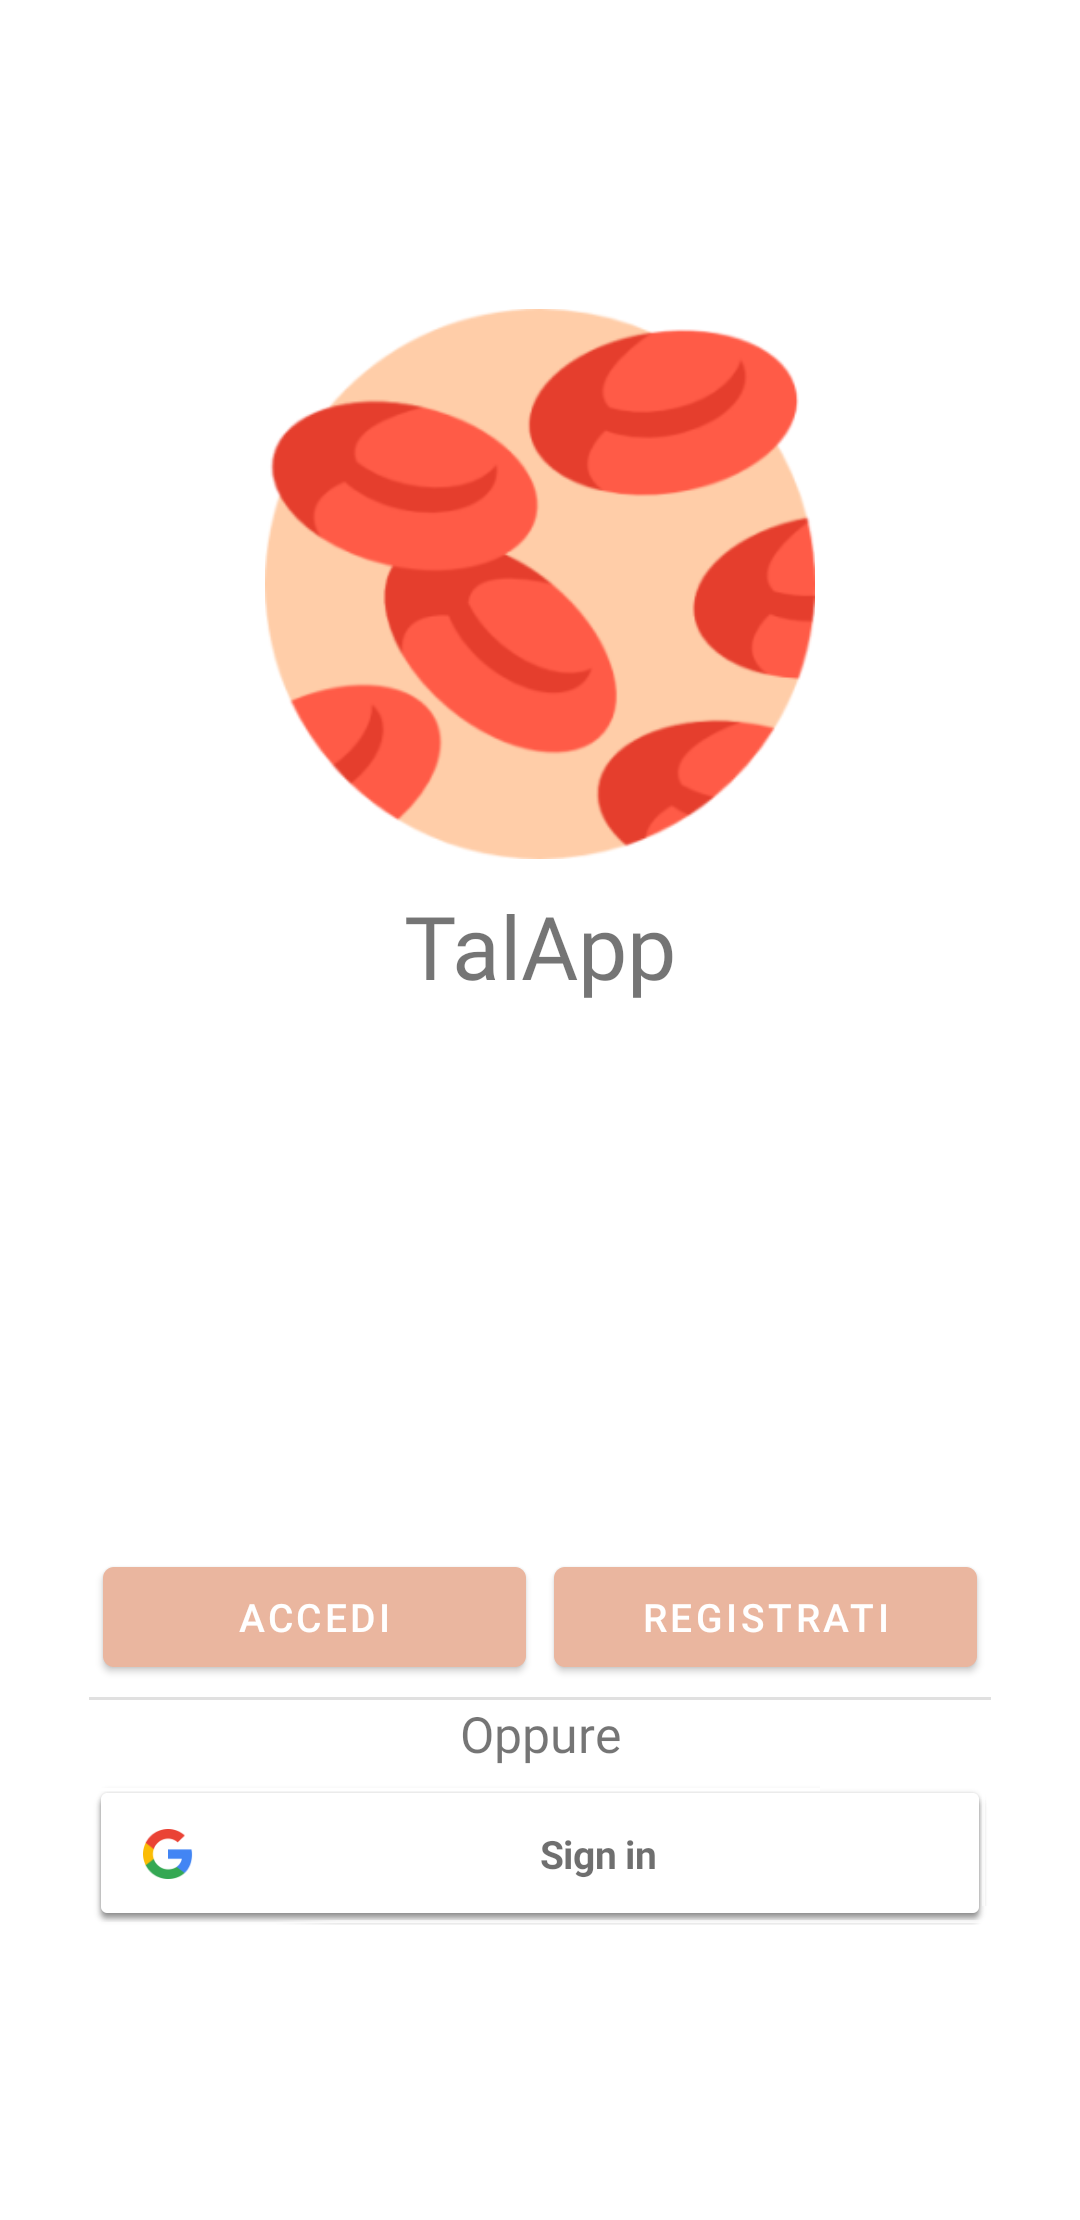
\includegraphics[width=.3\textwidth, keepaspectratio]{img/Screenshots/Accesso e registrazione/SchermataIniziale.png}
\caption{Schermata iniziale} \label{2.3}
\end{center}
\end{figure}

In figura \ref{2.4} sono presenti i possibili accessi: con mail e password oppure con un account Google pre-esistente. 

Nel primo caso [Fig. \ref{2.4a}] è utilizzato un login tramite mail e password, questi devono essere correttamente salvati nel database degli accessi - in caso contrario viene notificato un errore. 

Nel secondo caso [Fig. \ref{2.4b}] si utilizza l'account Google per effettuare il login o l'eventuale registrazione.

In fase di registrazione [Fig. \ref{2.4c}] è richiesta per la registrazione una mail - ancora non presente nel database degli accessi - e una password con le seguenti caratteristiche:
\begin{itemize}
    \item Lunghezza di almeno otto caratteri
    \item Almeno una lettera maiuscola
    \item Almeno una lettera minuscola
    \item Almeno un numero
    \item Almeno un carattere speciale, quali \$ ? \% \^ \& * ( ) \_ - + = @ ~ \#.
\end{itemize}
Le due password inserite devono coincidere onde evitare situazioni di errore.

\begin{figure}[H]
\centering
\subfloat[][\emph{Accesso con mail e password}]
{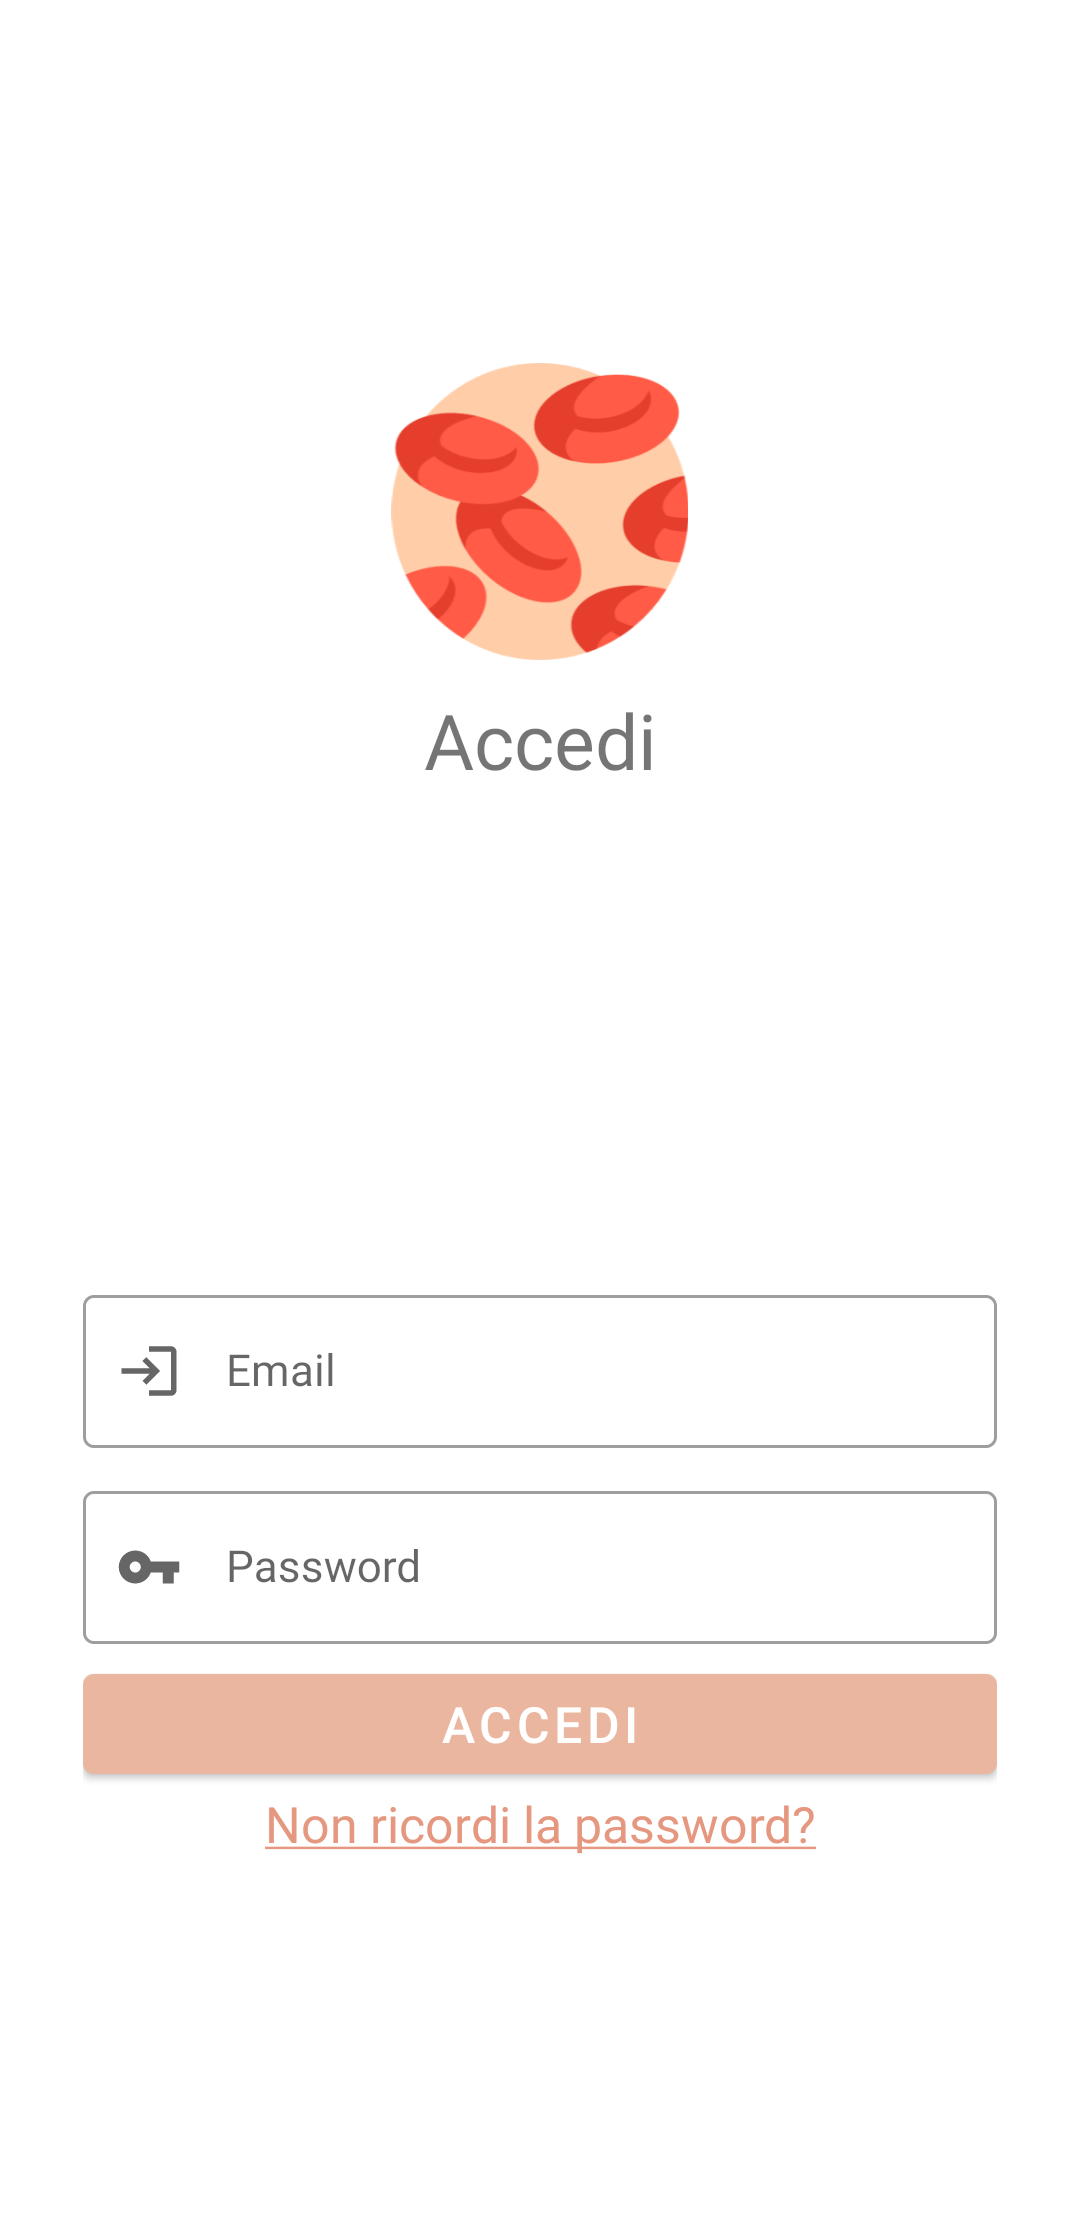
\includegraphics[width=.3\textwidth]{img/Screenshots/Accesso e registrazione/Accedi.png} \label{2.4a}} \quad
\subfloat[][\emph{Accesso con Google}]
{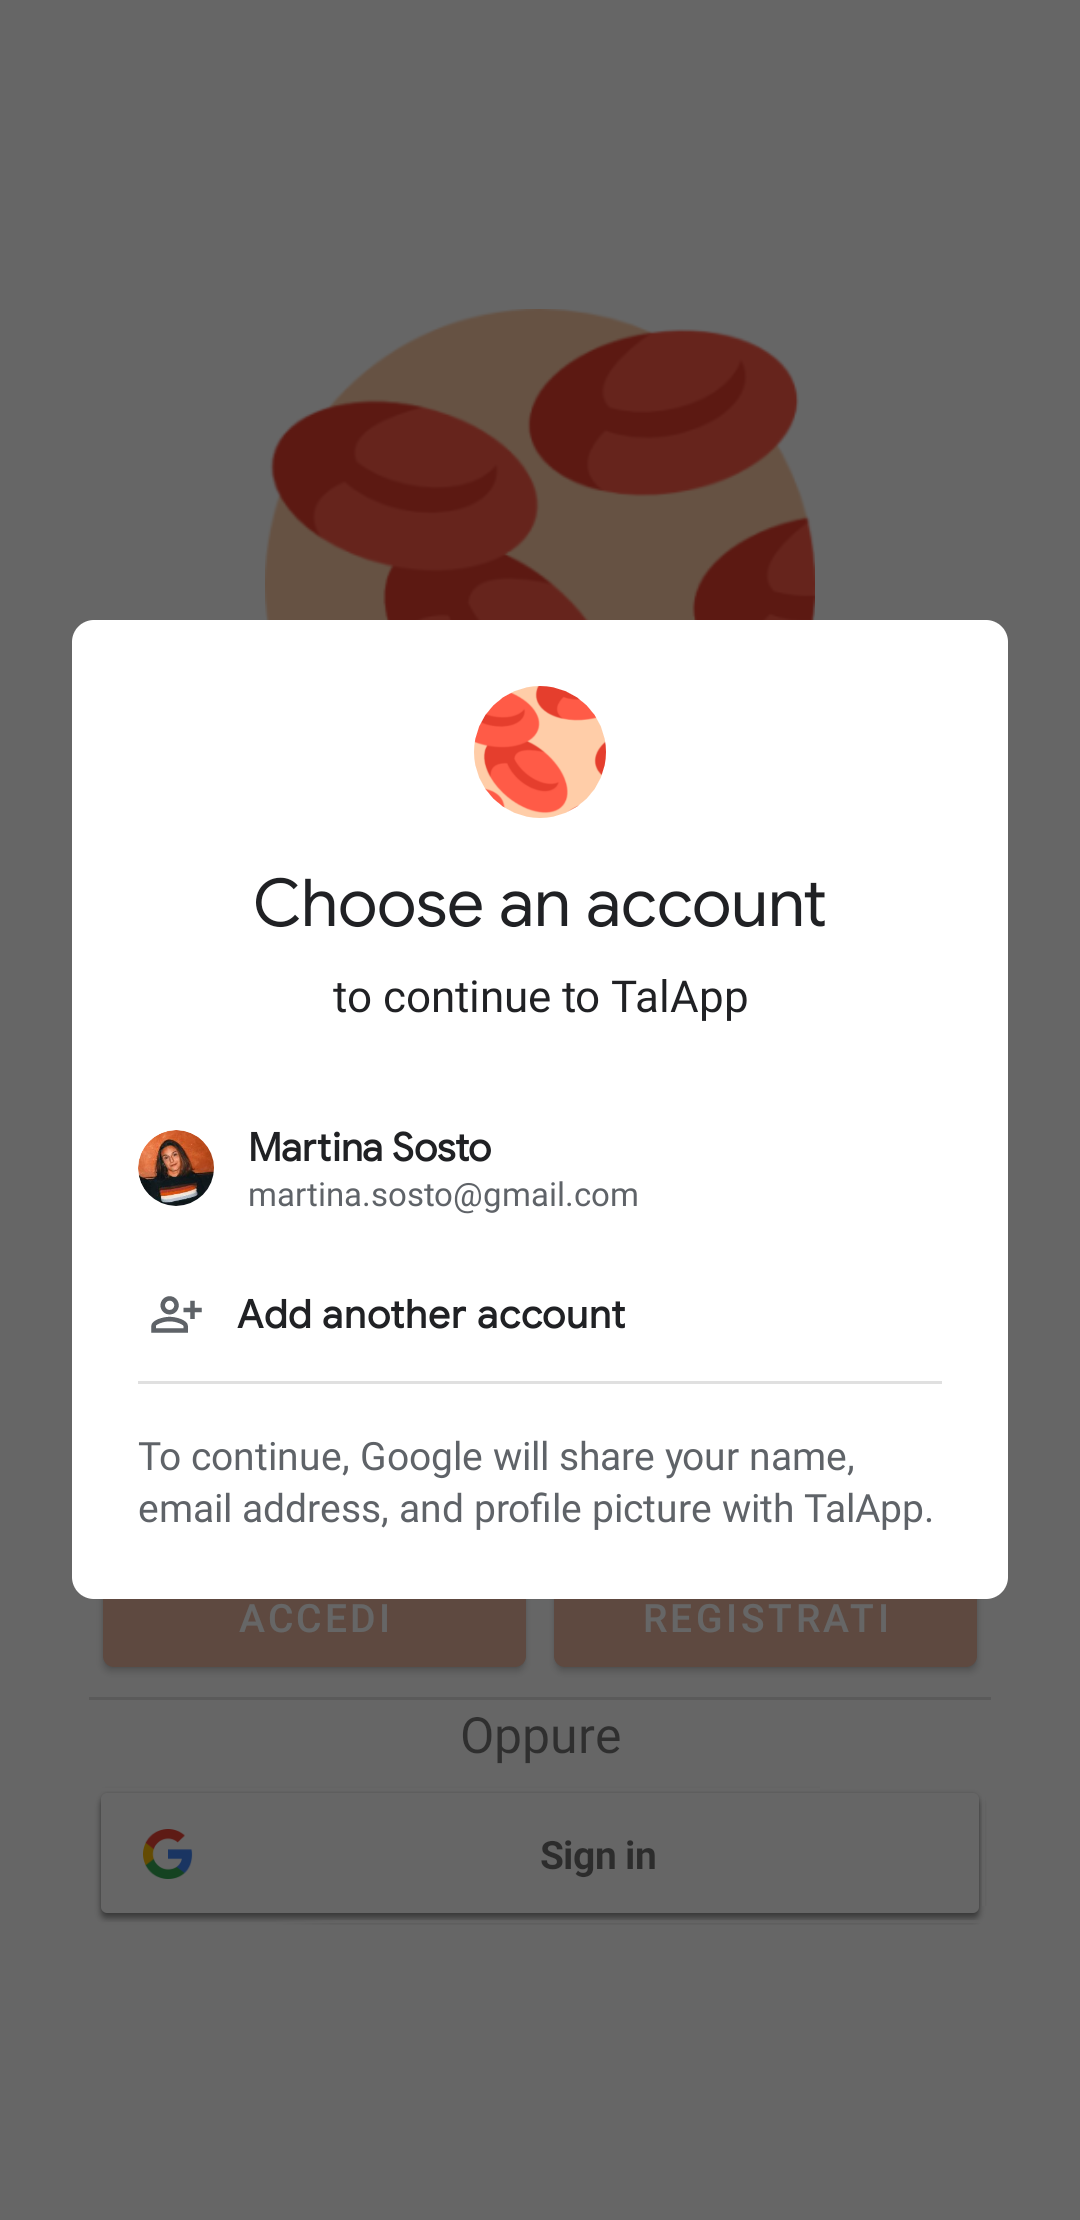
\includegraphics[width=.3\textwidth]{img/Screenshots/Accesso e registrazione/AccediGoogle.png} \label{2.4b}} \quad
\subfloat[][\emph{Registrazione}]
{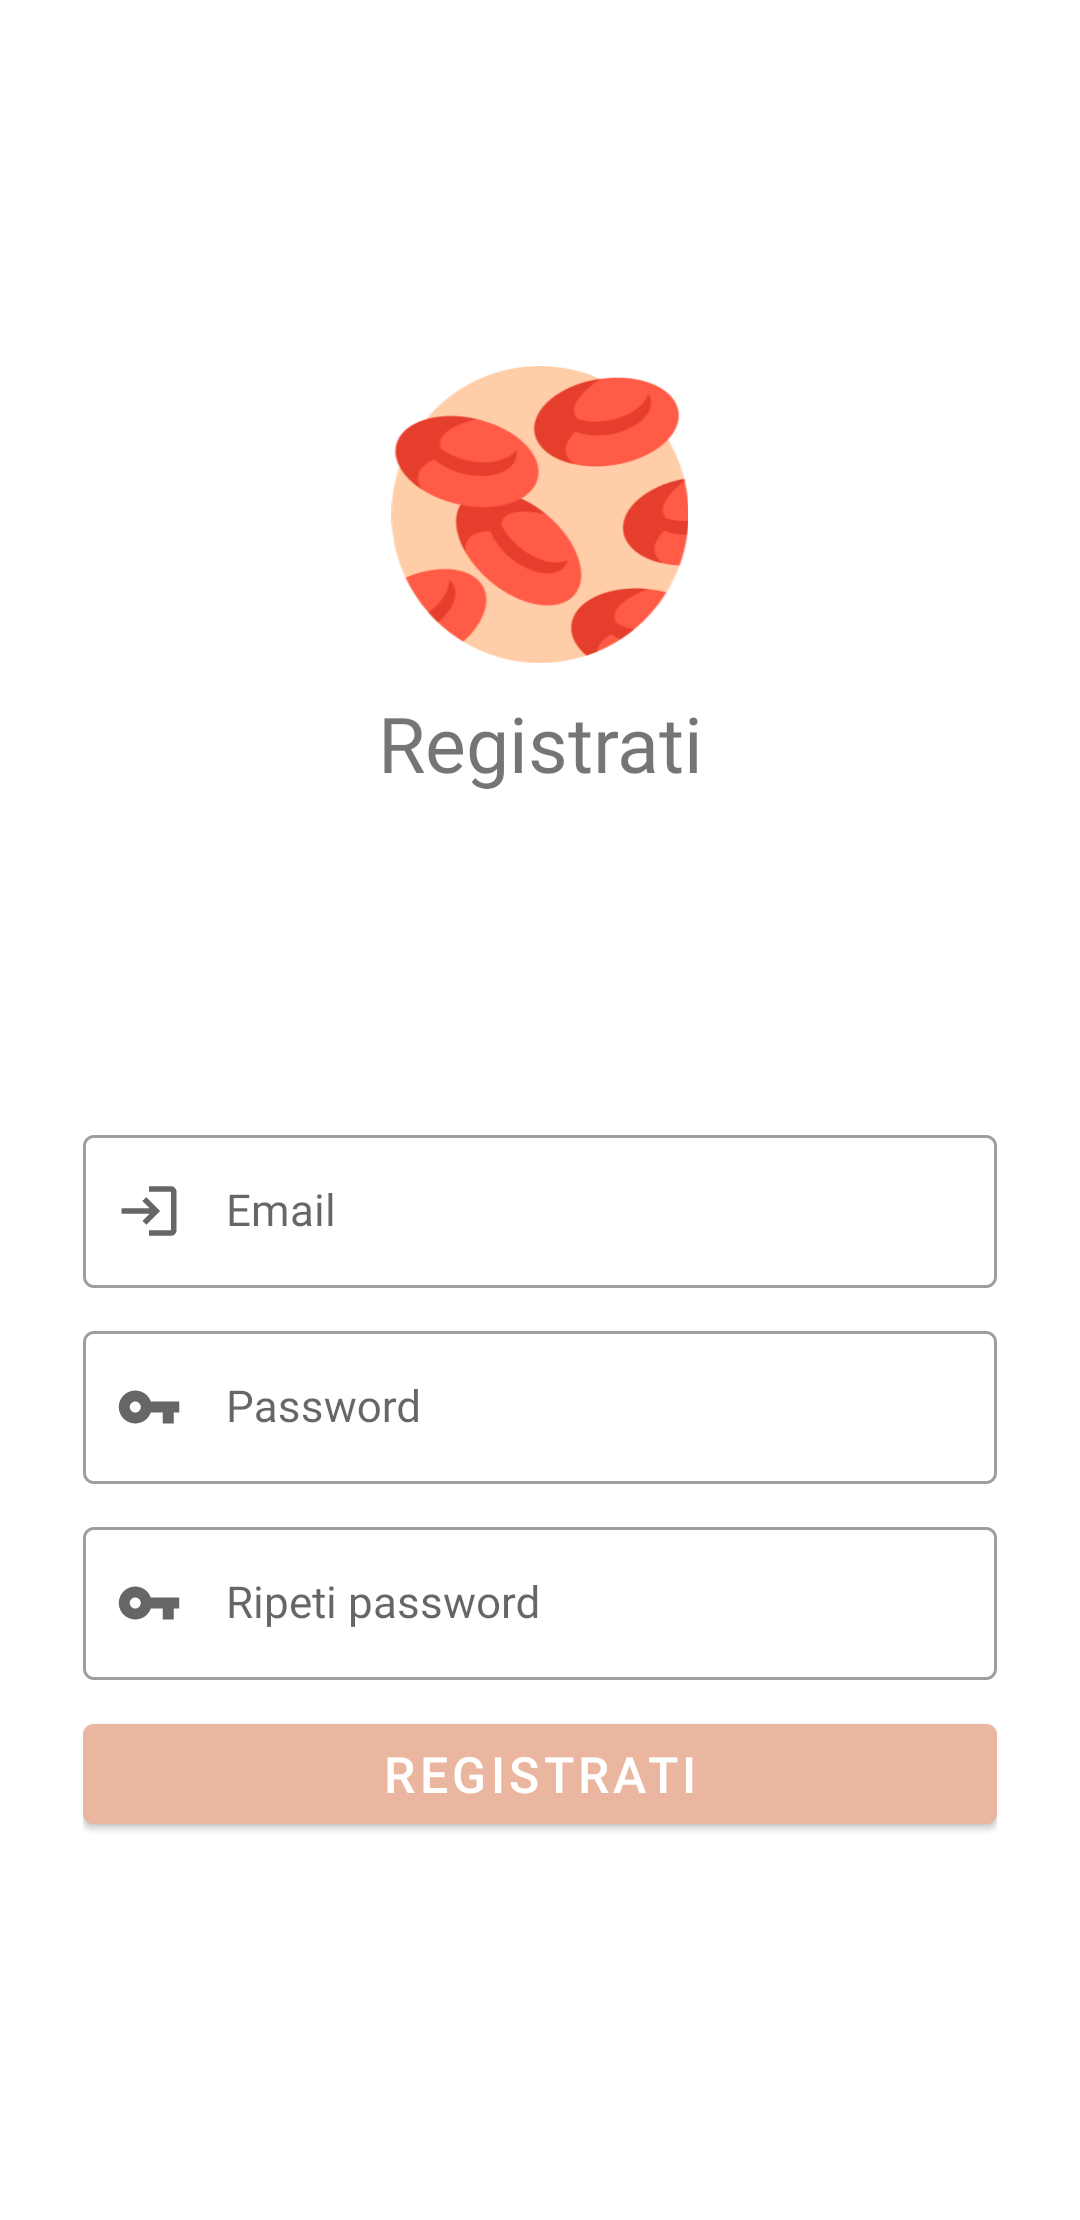
\includegraphics[width=.3\textwidth]{img/Screenshots/Accesso e registrazione/Registrati.png} \label{2.4c}} \quad
\caption{Schermate di accesso e registrazione}
\label{2.4}
\end{figure}

In fase di accesso si ha modo di richiedere il recupero password, avviando il procedimento mostrato in figura \ref{ripristino}, operazione possibile tramite un meccanismo fornito da Firebase Authantication.

\subsubsection{Recupero password}
Toccando su ``Recupera password'' si passa alla schermata di recupero delle credenziali [Fig. \ref{ripristinoA}], l'inserimento della mail permette l'invio di un link [Fig. \ref{ripristinoB}] nella casella di posta dell'utente, per via di questo si ha modo di modificare la password.

\begin{figure}[H]
\centering
\subfloat[][\emph{Schermata password dimenticata}]
{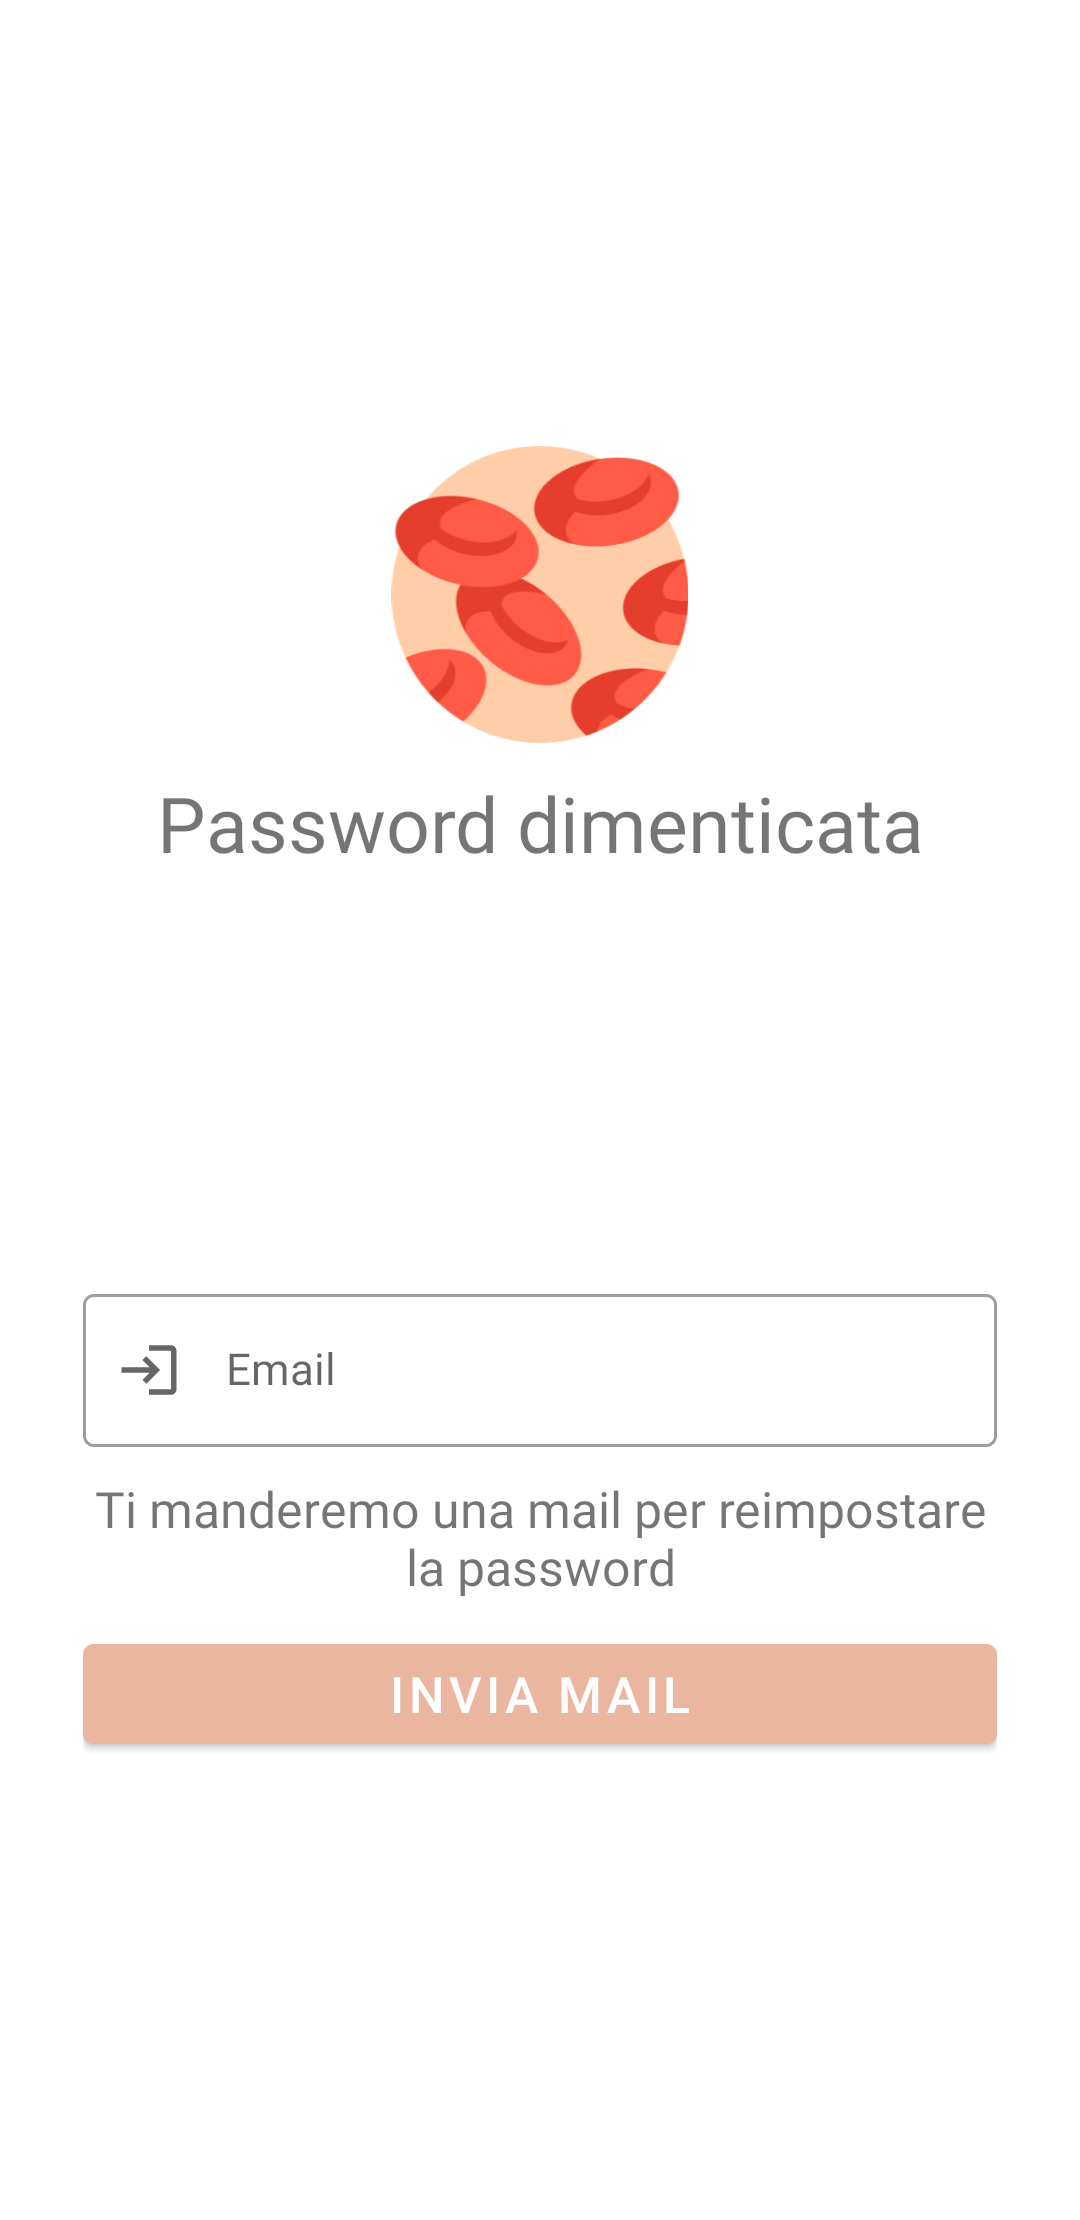
\includegraphics[width=.3\textwidth]{img/Screenshots/Accesso e registrazione/PasswordDimenticata.png} \label{ripristinoA}} \quad
\subfloat[][\emph{Mail di ripristino password}]
{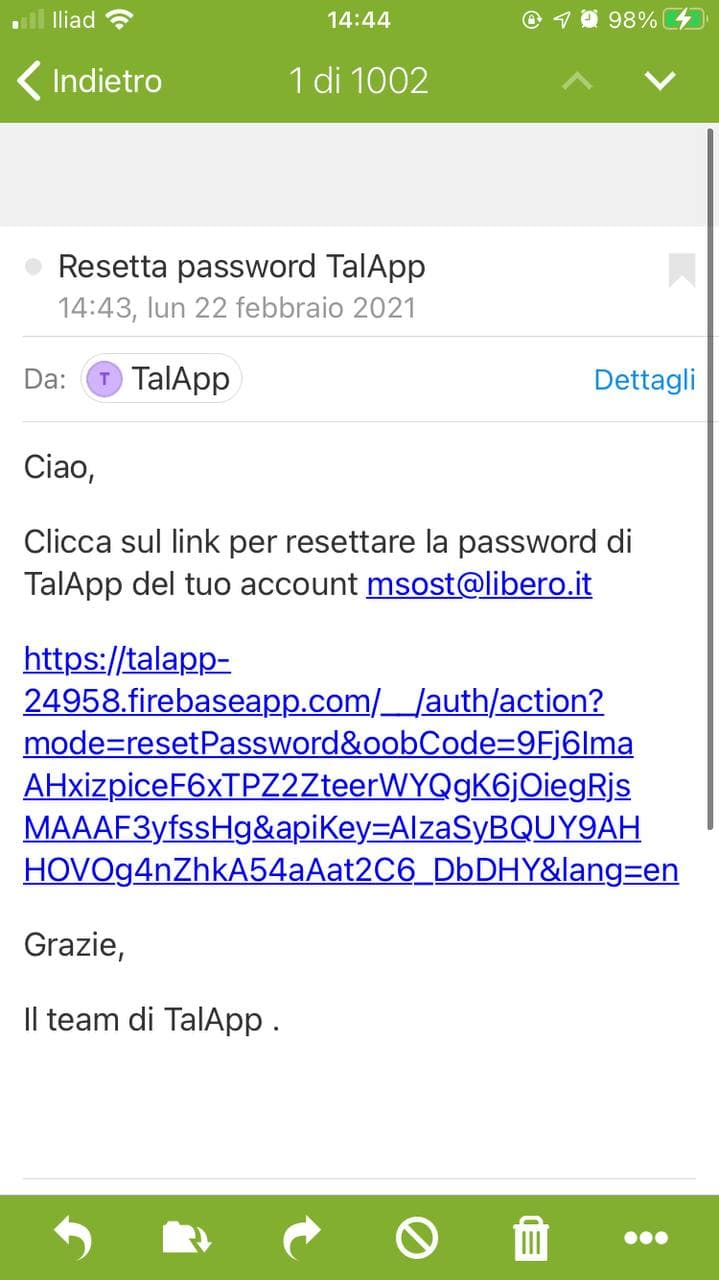
\includegraphics[width=.3\textwidth]{img/Screenshots/Accesso e registrazione/PasswordDimenticataMail.png} \label{ripristinoB}} \quad
\caption{Schermate di ripristino password}
\label{ripristino}
\end{figure}

%SchermataIniziale
%Accedi
%AccediGoogle
%Registrati
%PasswordDimenticata
%PasswordDimenticataMail

\subsection{Home e calendario}
Una volta effettuato il login correttamente, l'utente può gestire la sua cartella clinica in base alle categorie Trasfusioni, Esami e Terapie [Fig. \ref{home}].
Tramite il calendario si accede a una sezione dedicata alla gestione temporale degli eventi, consente di avere una visione totale dei dati mensili.
L'icona dell'ingranaggio in alto a destra concede di navigare nelle impostazioni, maggiori informazioni si trovano al paragrafo 2.3.7.

\begin{figure}[H]
\begin{center}
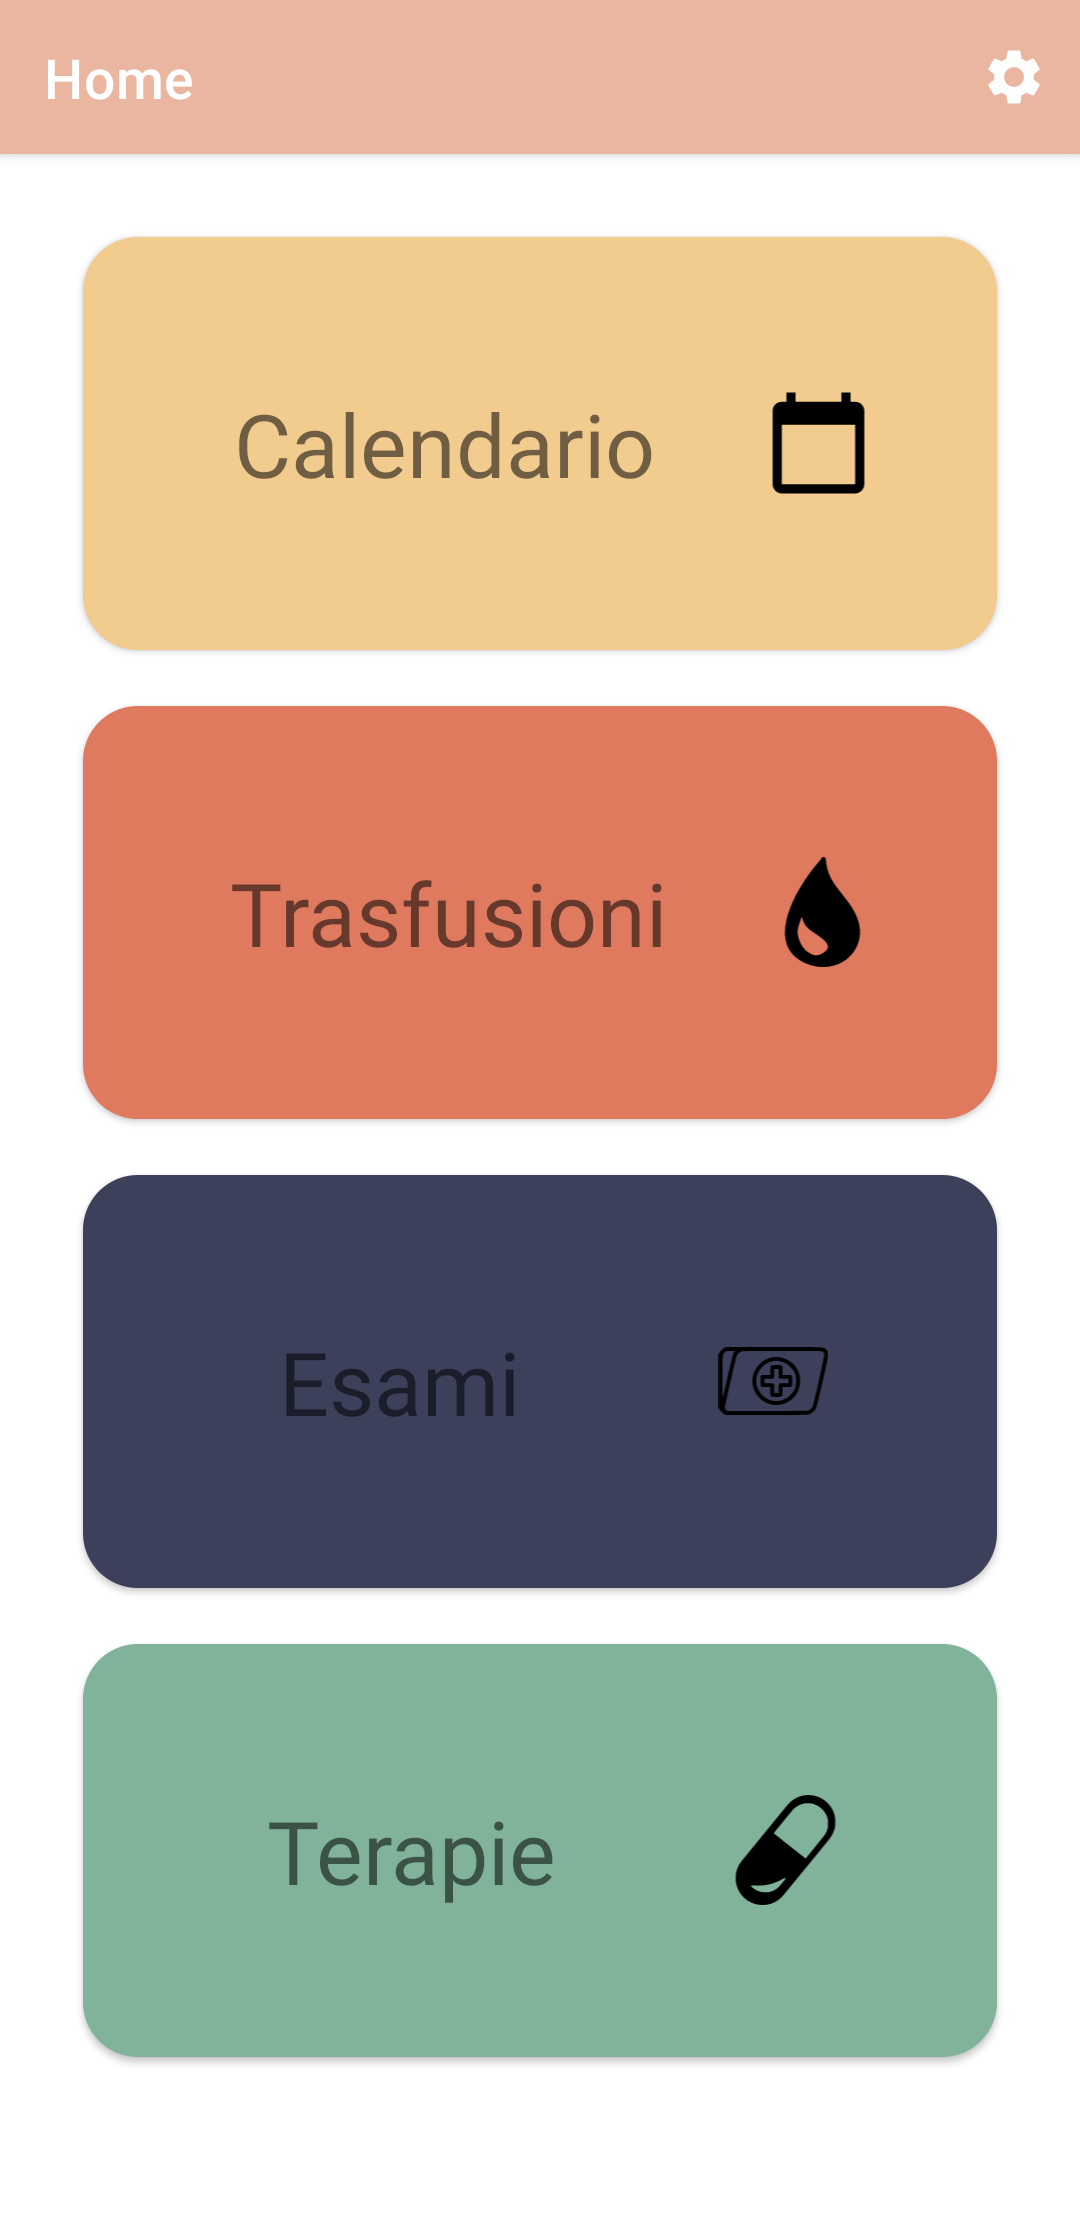
\includegraphics[width=.3\textwidth, keepaspectratio]{img/Screenshots/Home e calendario/Home.png}
\caption{Schermata Home} \label{home}
\end{center}
\end{figure}

In figura \ref{calendarioA} il calendario funge come elemento di raccordo degli eventi mensili, inizialmente il periodo in questione è sempre il mese corrente, tramite le frecce laterali si passa a quelli precedenti o successivi. L'icona contente il simbolo della somma abilita le funzionalità di aggiunta degli eventi.

In ogni giorno del calendario sono presenti delle icone raffigurative degli impegni giornalieri, il colore varia in base alla tipologia di evento. Selezionando la casella di un giorno preciso si mostra la lista degli eventi che lo riguardano [Fig. \ref{calendarioB}], è divisa per tipologia ed è contornata dal colore di riferimento. Ogni elemento presenta le informazioni che lo caratterizzano.

Sulla barra di ricerca in alto si cercano parole chiave contenute negli eventi, anche questi come nel caso precedente sono ordinati per tipologia [Fig. \ref{calendarioC}].

\begin{figure}[H]
\centering
\subfloat[][\emph{Calendario}]
{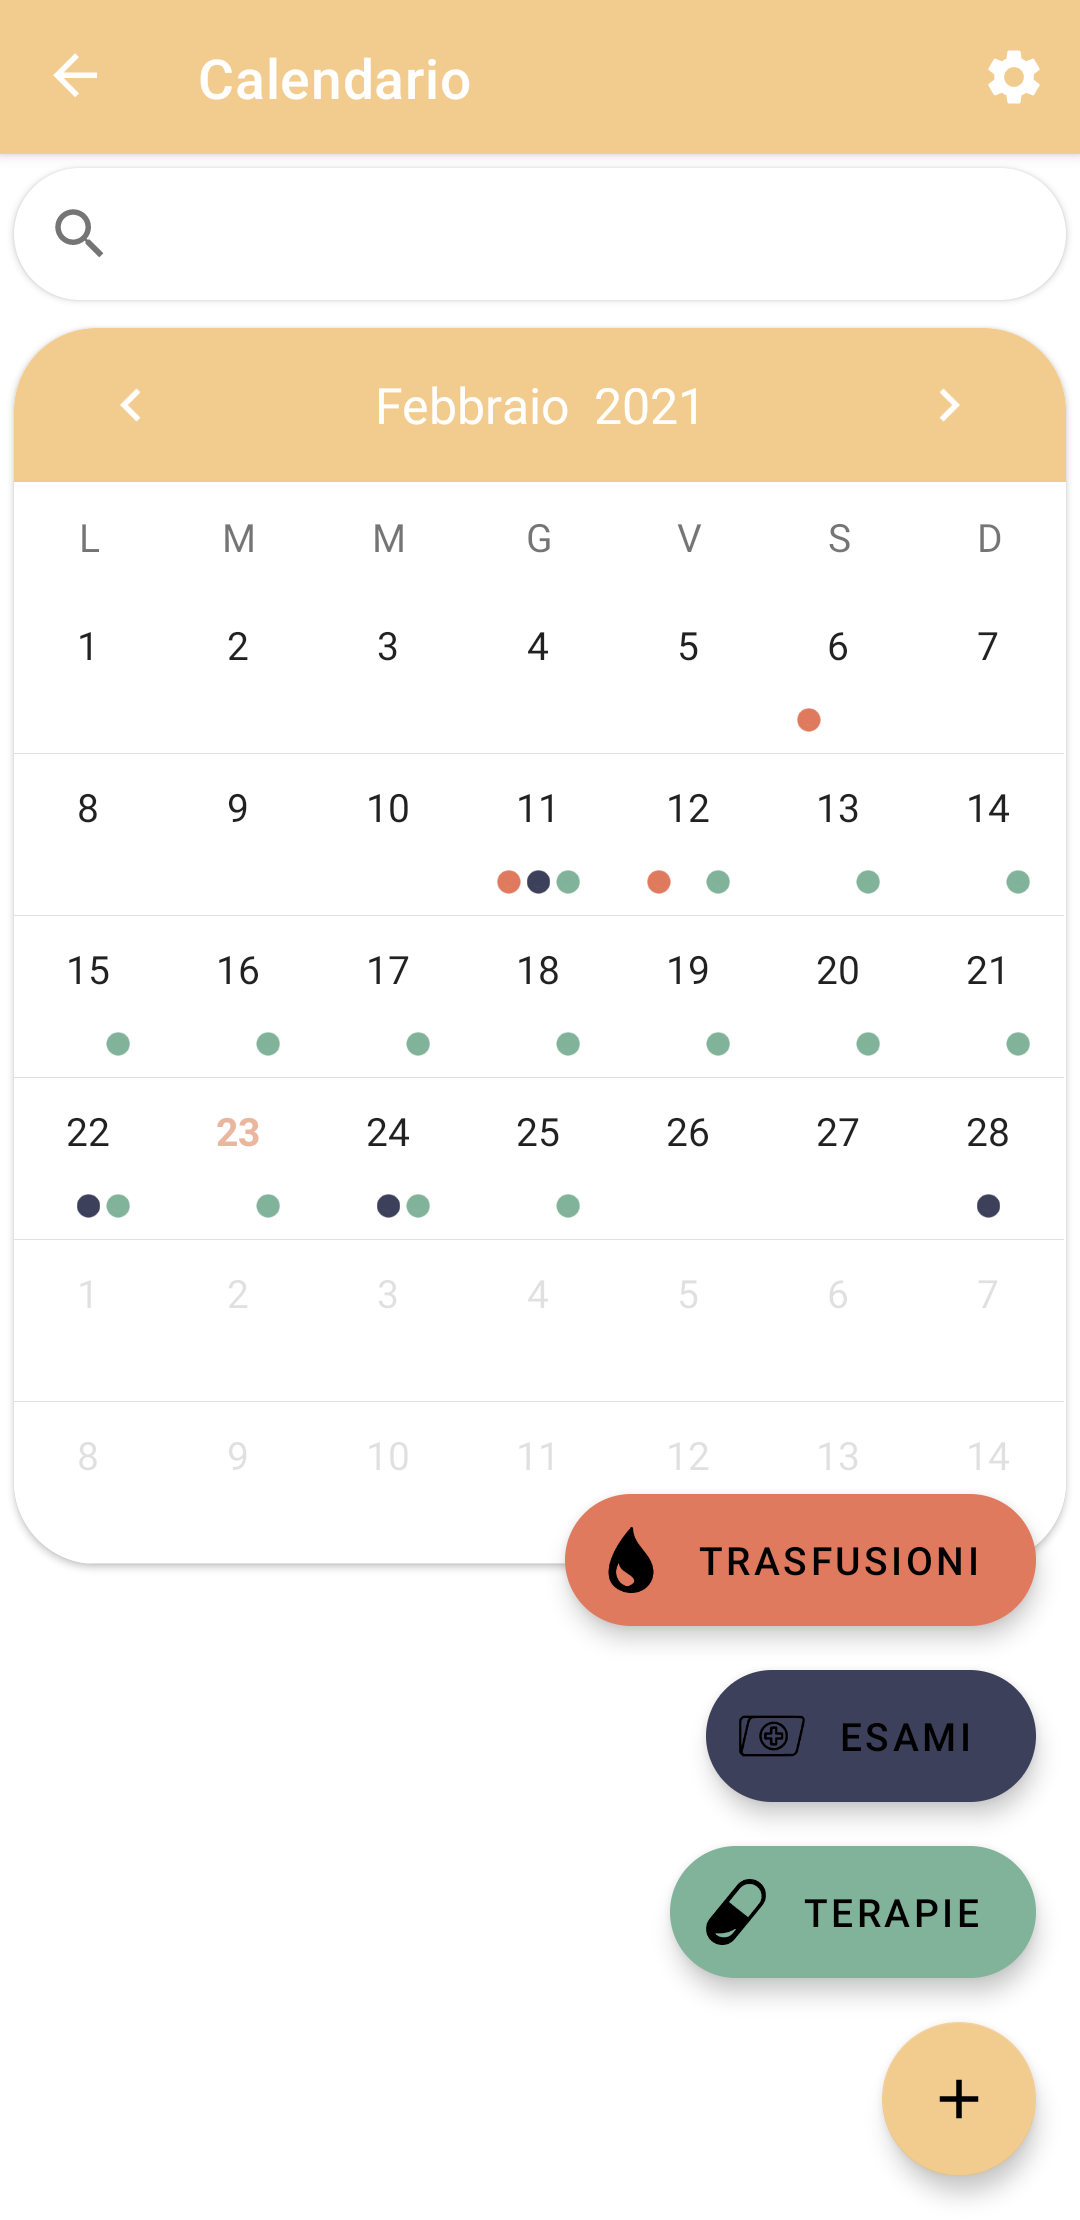
\includegraphics[width=.3\textwidth]{img/Screenshots/Home e calendario/Calendario.png} \label{calendarioA}} \quad
\subfloat[][\emph{Eventi del giorno}]
{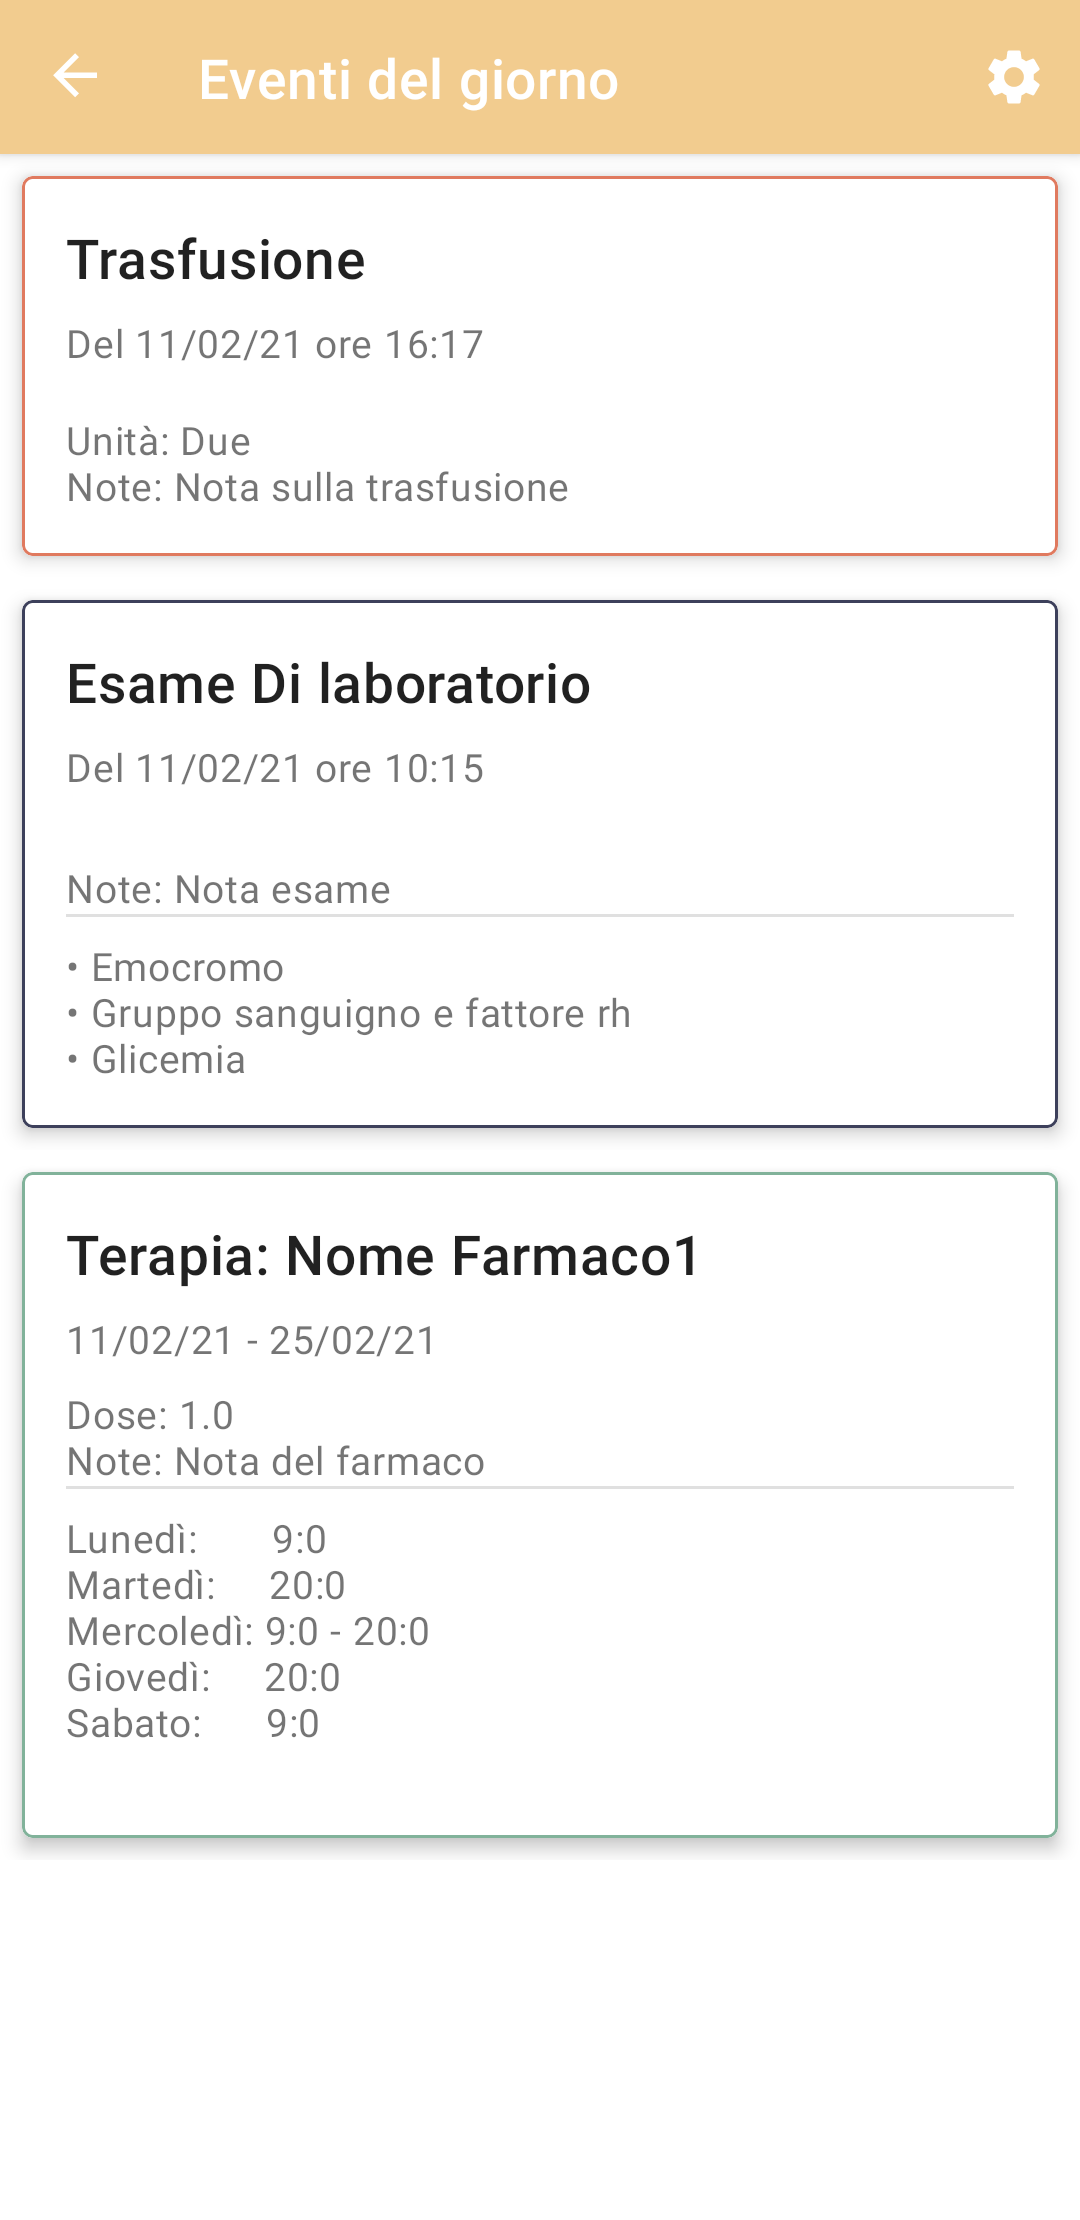
\includegraphics[width=.3\textwidth]{img/Screenshots/Home e calendario/EventiDelGiorno.png} \label{calendarioB}} \quad
\subfloat[][\emph{Barra di ricerca}]
{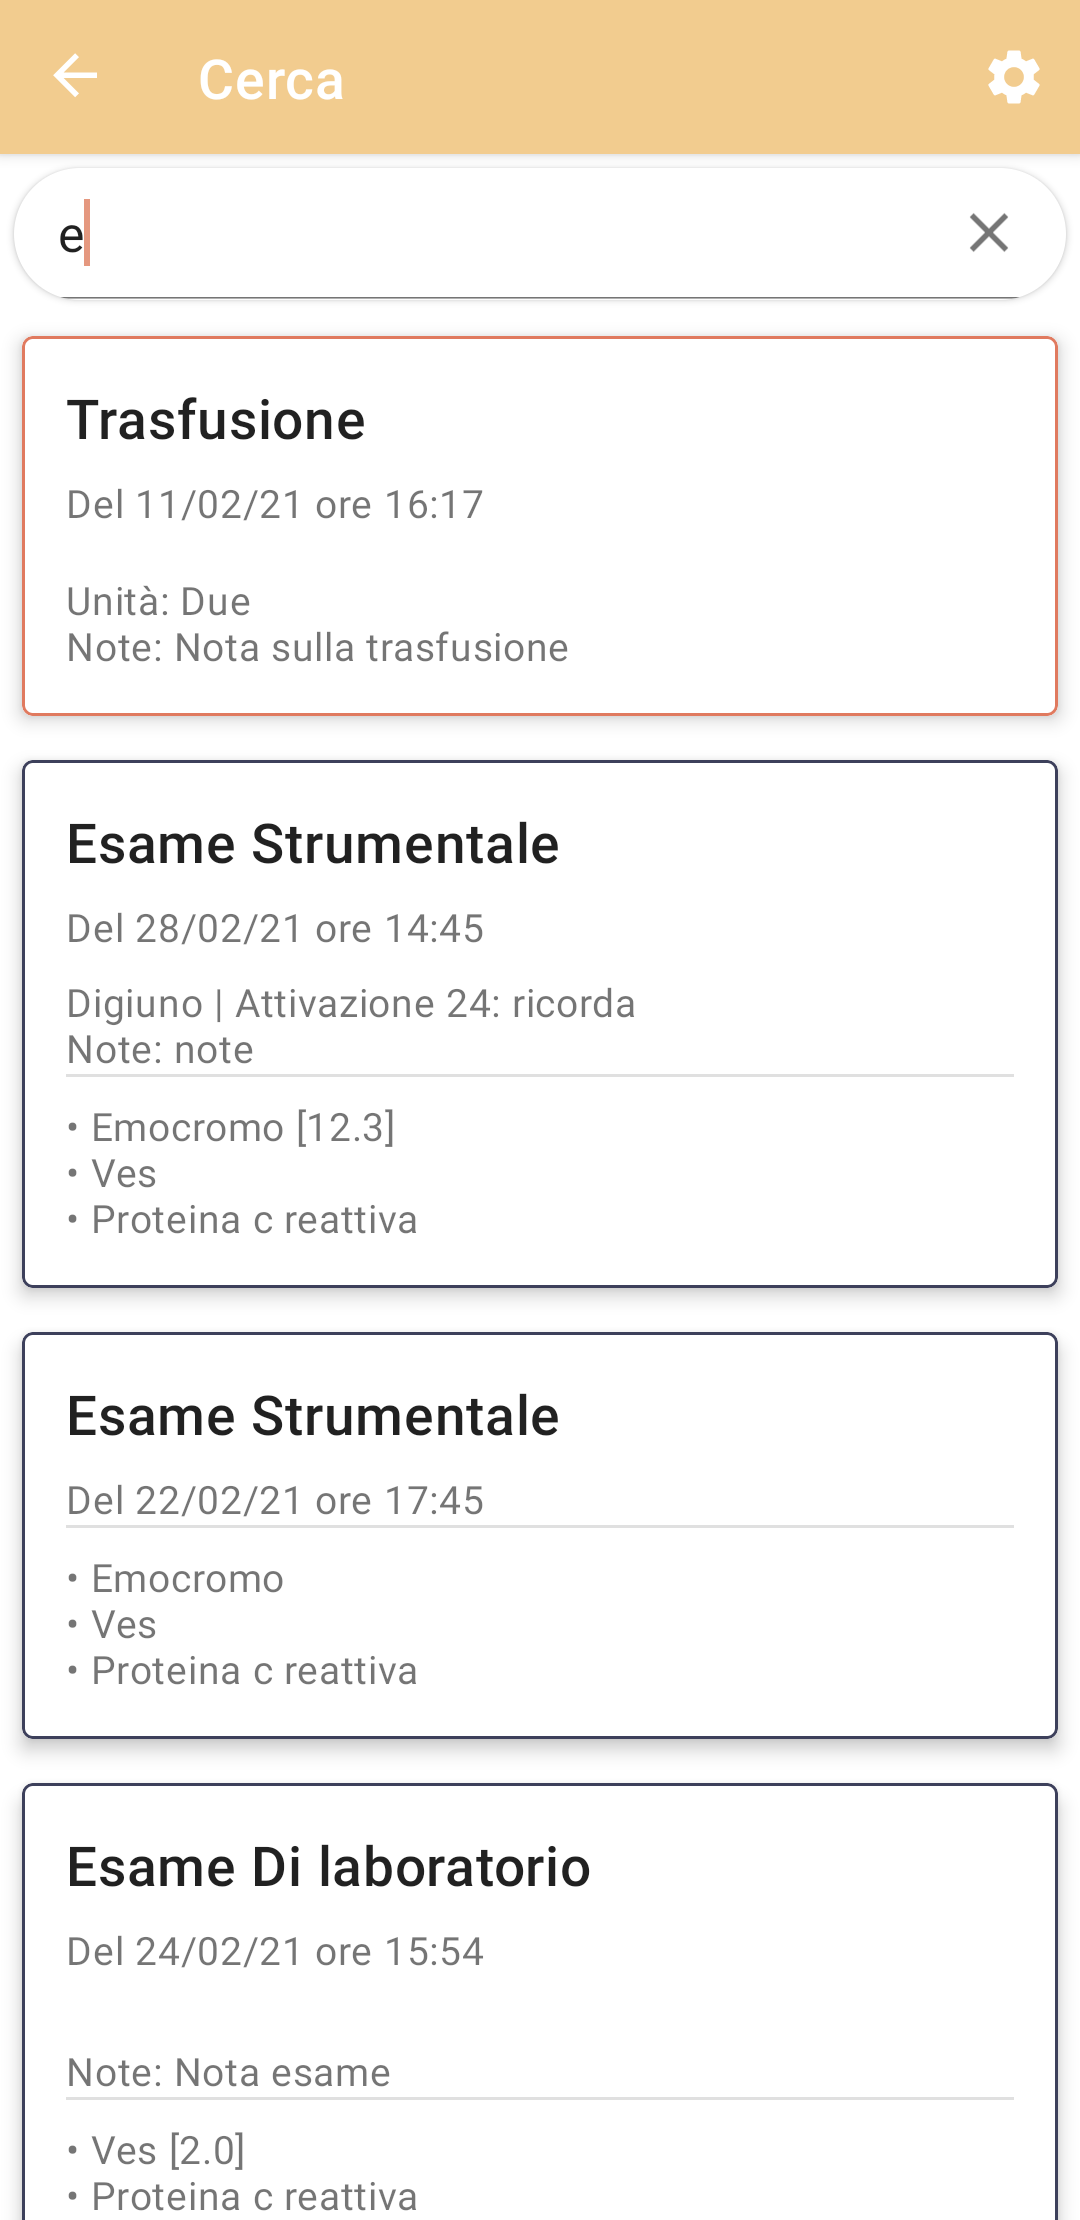
\includegraphics[width=.3\textwidth]{img/Screenshots/Home e calendario/Cerca.png} \label{calendarioC}} \quad
\caption{Schermata del calendario}
\label{calendario}
\end{figure}

%Home
%Calendario
%Cerca
%EventiDelGiorno

\subsection{Trasfusioni}
La schermata delle trasfusioni è raggiungibile dalla home e permette di avere una visione completa degli eventi trasfusionali [Fig. \ref{trasfusioniA}].

In alto è sempre presente la componente che permette di aggiungere nuove trasfusioni.

Al di sotto è situata una barra progressiva, questa segnala al paziente la data ultima e successiva in cui dovrà svolgere la terapia trasfusionale. Se non ci sono dati a sufficienza per questa rappresentazione, viene mostrata solo una delle due date oppure un avviso che esplicita la mancanza delle informazioni necessarie. Sotto la barra vengono indicati i giorni mancanti al prossimo appuntamento, se presente. Gli eventi futuri vengono elencati in una lista [Fig. \ref{trasfusioniB}].

Se nel database sono presenti dati riguardanti le terapie trasfusionali passate, viene aggiunta alla schermata la componente che permette di aggiornarne i valori e il pulsante che dà accesso alla cronologia.

I valori dell'Hb (emoglobina) vengono raccolti in un grafico a fine schermata [Fig. \ref{trasfusioniB}]. 

\begin{figure}[H]
\centering
\subfloat[]
{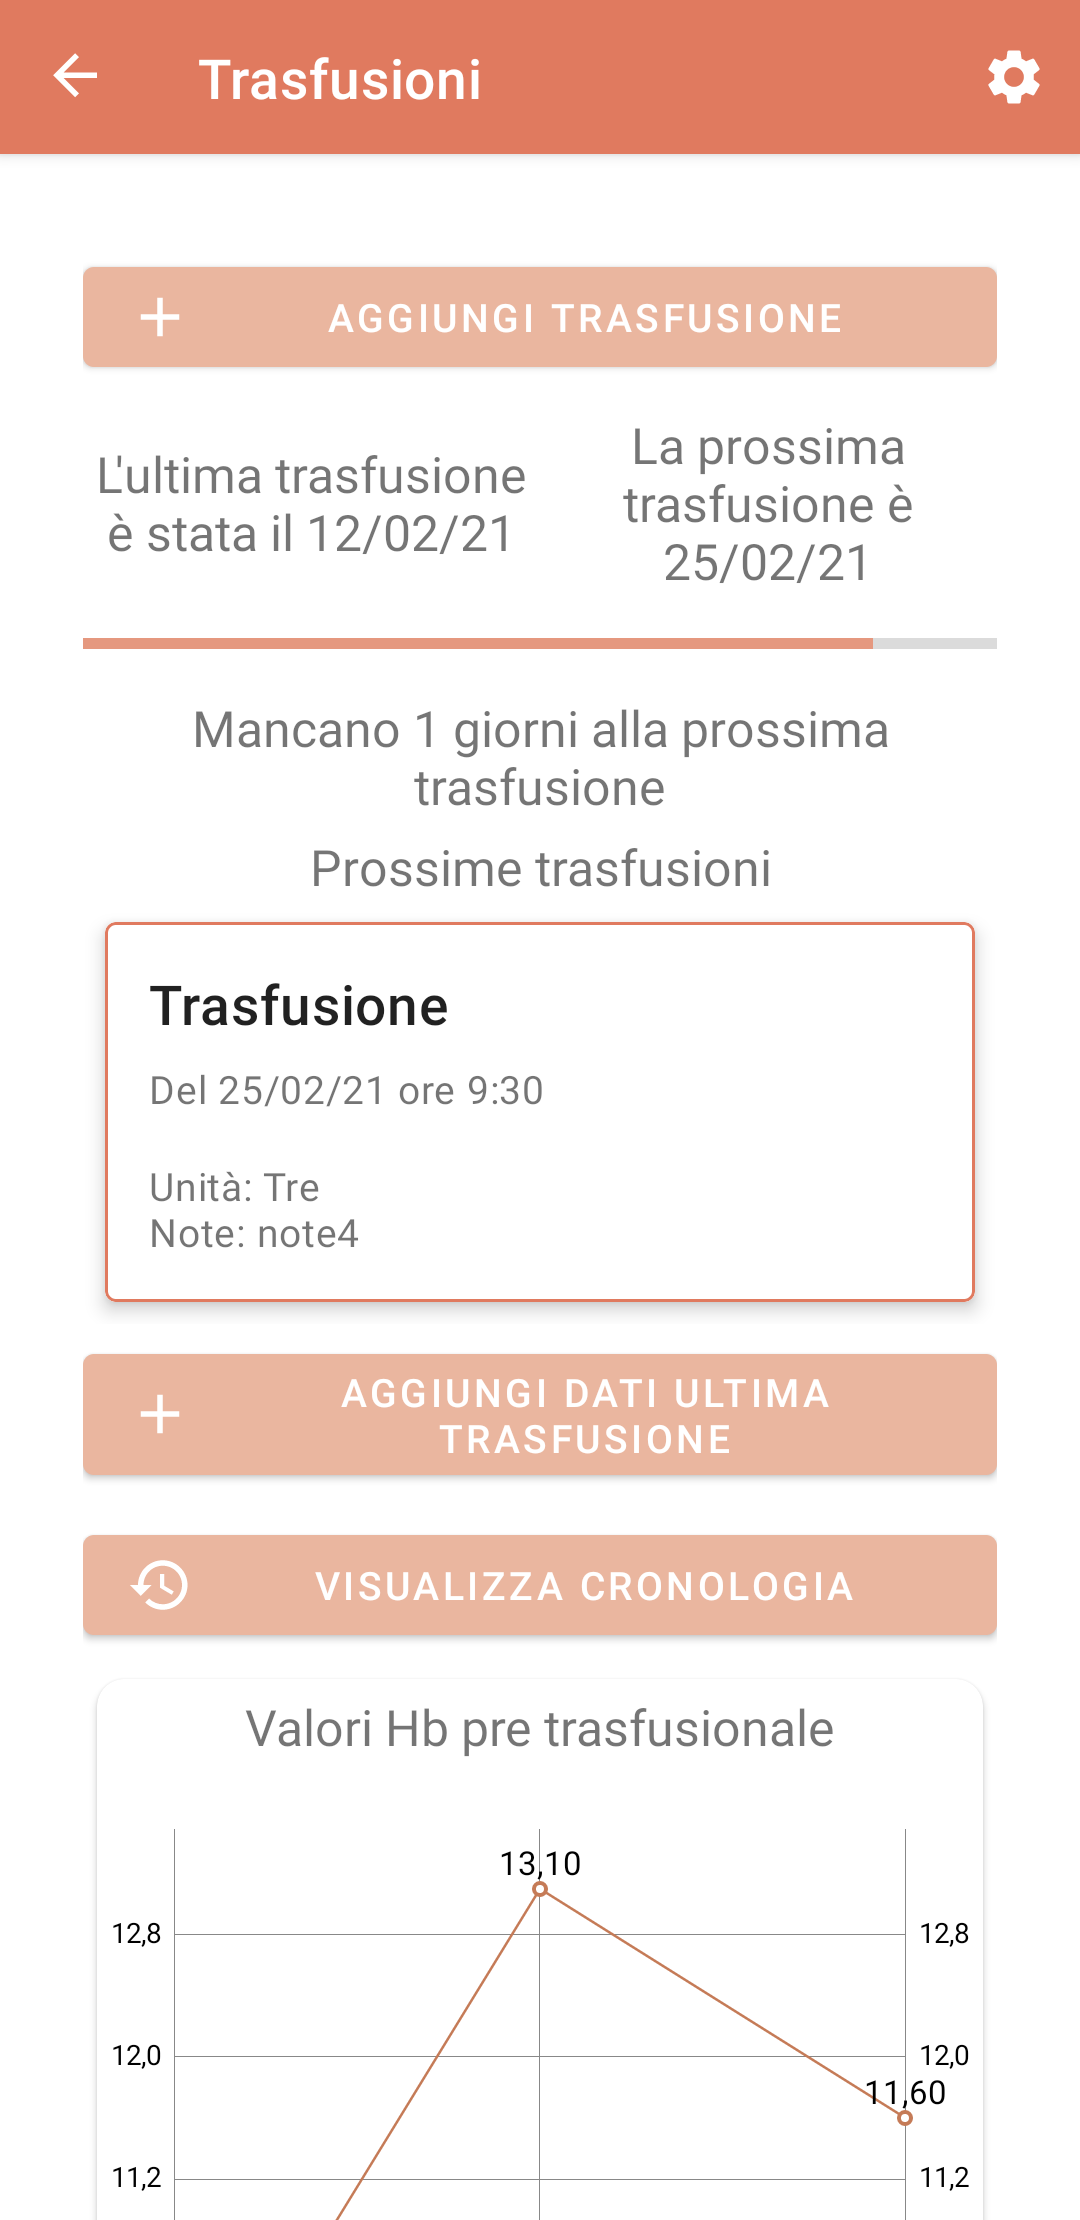
\includegraphics[width=.3\textwidth]{img/Screenshots/Trasfusioni/Fragment2.png} \label{trasfusioniA}} \quad
\subfloat[]
{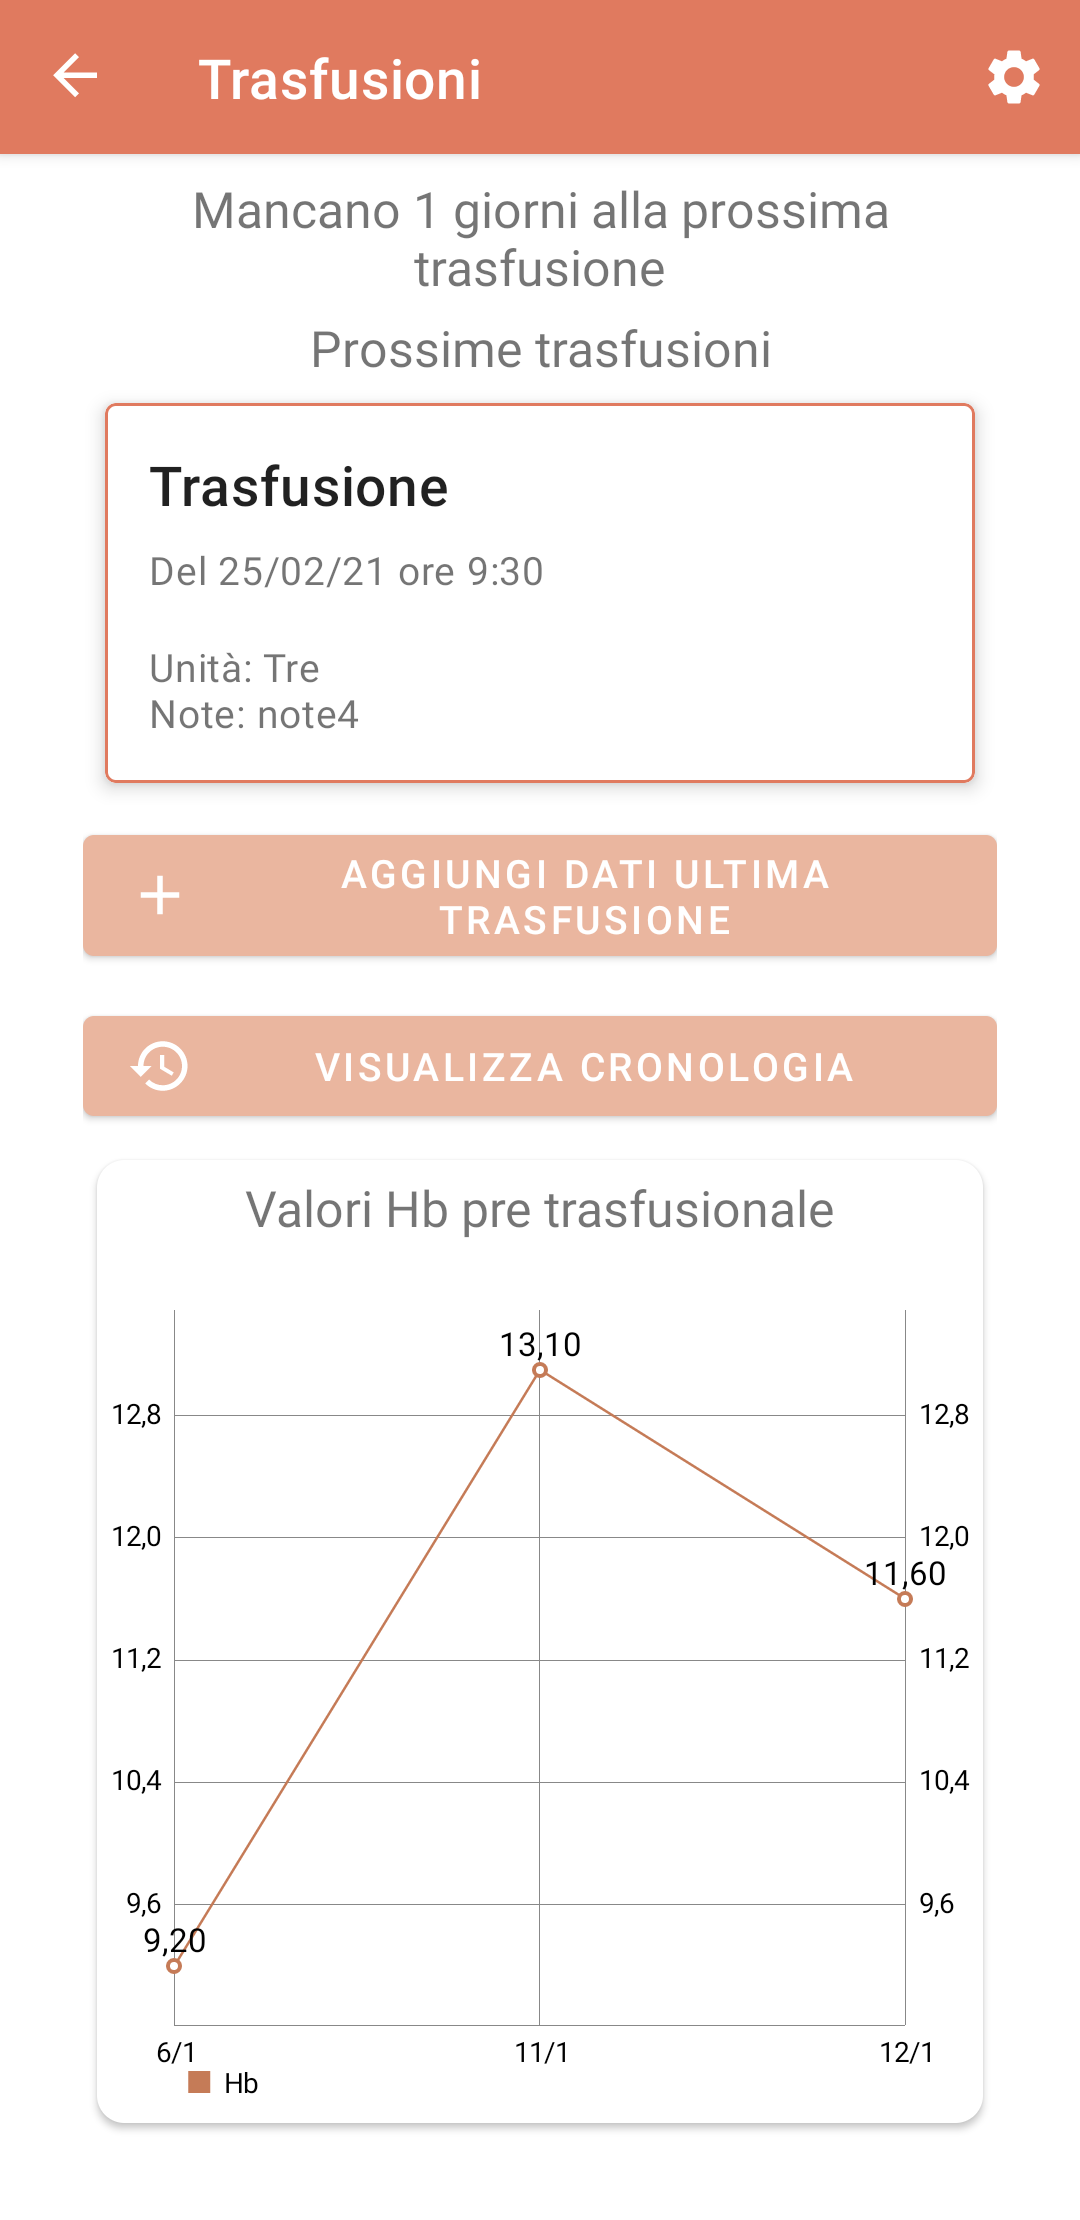
\includegraphics[width=.3\textwidth]{img/Screenshots/Trasfusioni/Fragment1.png} \label{trasfusioniB}} \quad
\caption{Schermata dedicata alle trasfusioni}
\label{trasfusioni}
\end{figure}

L'operazione di aggiunta di una trasfusione [Fig. \ref{trasfusioni1A}] è raggiungibile sia dal layout del calendario che dalla schermata di gestione delle stesse. Per l'inserimento bisogna indicare obbligatoriamente la data e l'ora dello svolgimento del trattamento, si può inoltre specificare quante unità di sangue sono previste e aggiungere ulteriori note.

Per mezzo di un tocco sul riquadro evento di una trasfusione si è in grado di modificarla [Fig. \ref{trasfusioni1B}]. La modifica dell'evento è effettuabile in diverse parti della piattaforma: nella schermata generale [Fig. \ref{trasfusioni}], nella cronologia [Fig. \ref{trasfusioni1C}] o nella visualizzazione degli eventi giornalieri [Fig. \ref{calendarioB}]. Modificando un evento passato si sblocca la possibilità di aggiungere informazioni riguardanti l'emoglobina pre-trasfusionale.

Si accede alla cronologia di un qualsiasi evento solo dalla schermata principale in considerazione, in questo caso quella in figura \ref{trasfusioni}. La cronologia elenca gli eventi in ordine temporale inverso - ovvero dal più al meno recente.

\begin{figure}[H]
\centering
\subfloat[][\emph{Aggiunta}]
{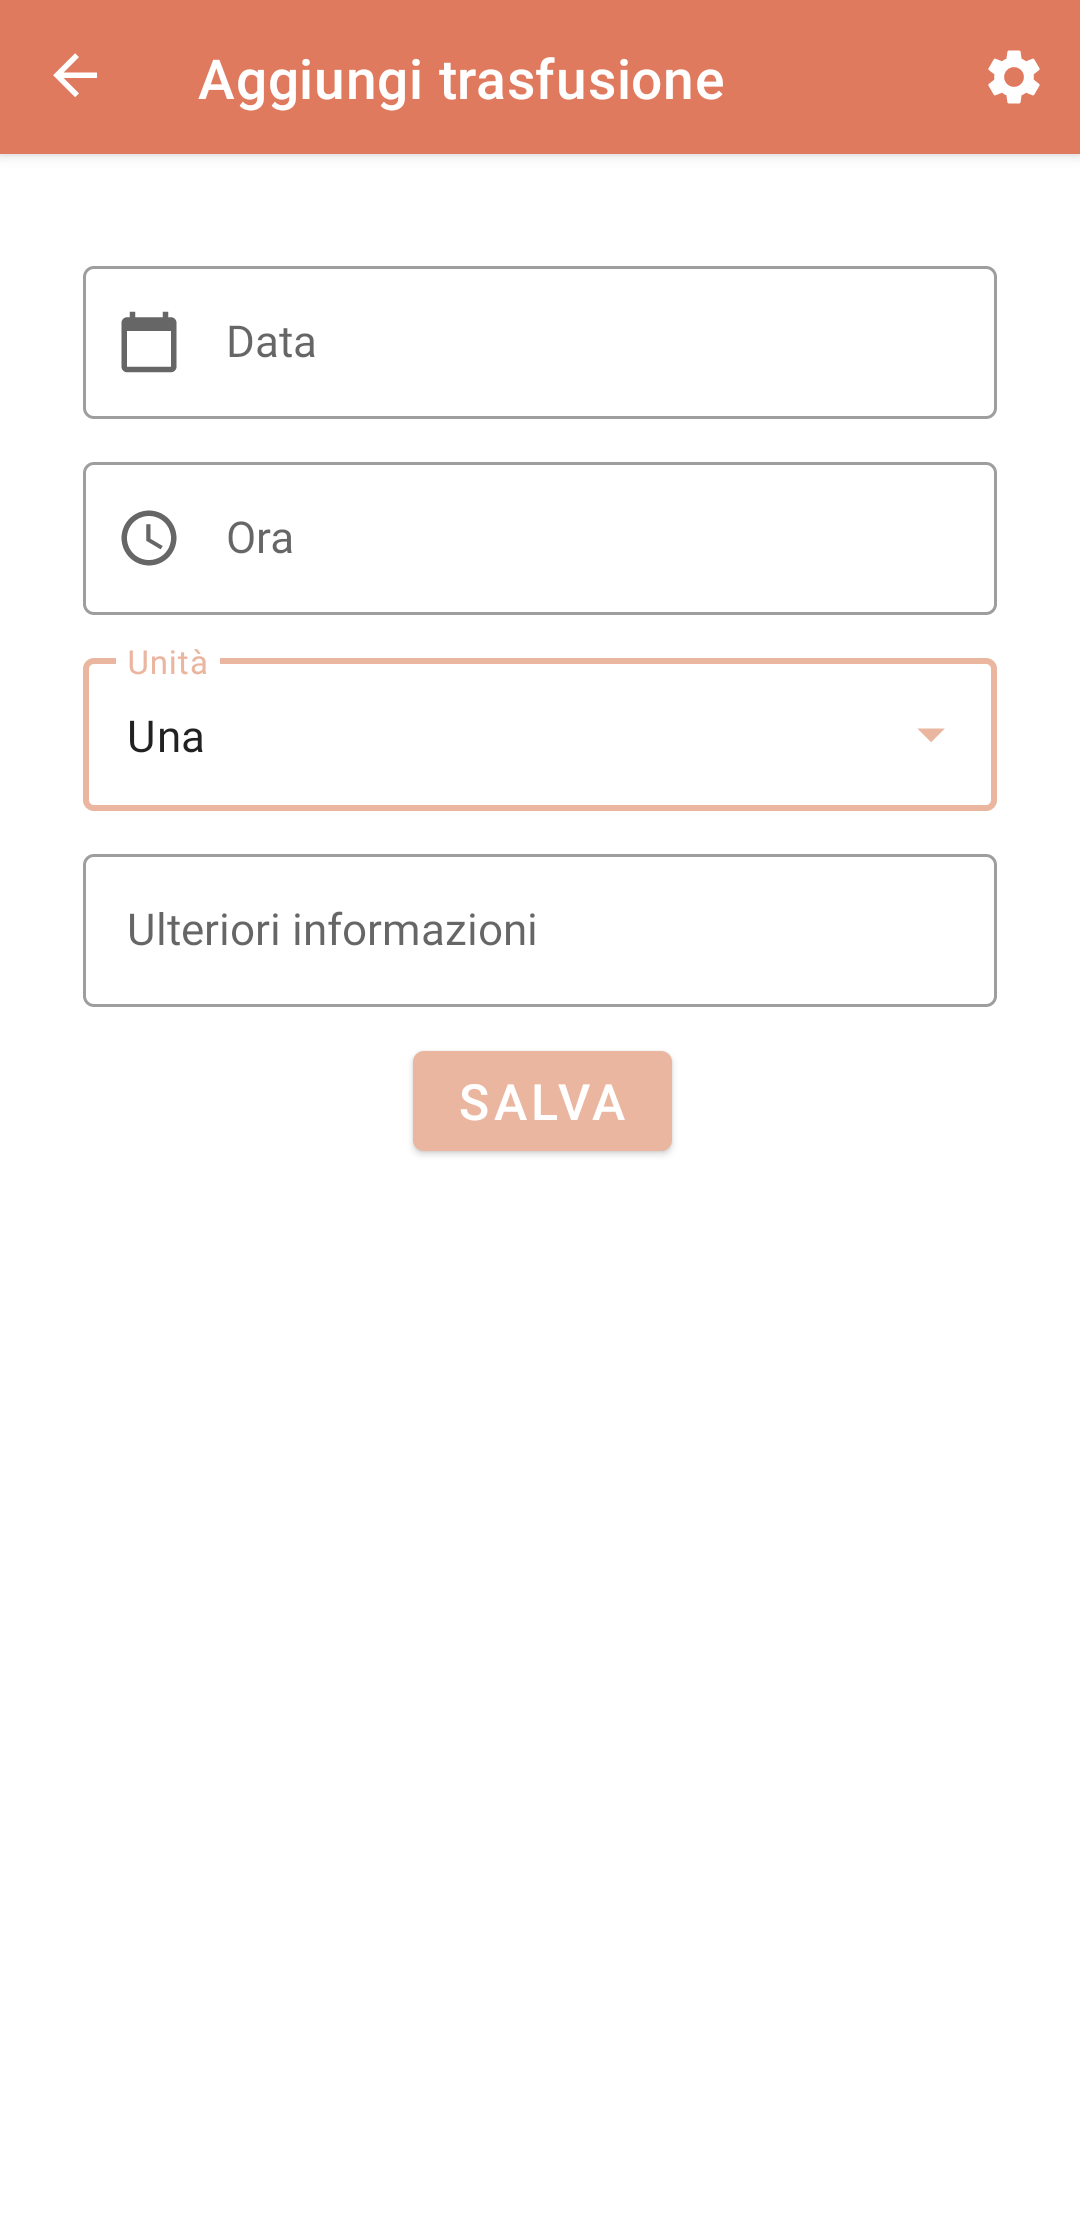
\includegraphics[width=.3\textwidth]{img/Screenshots/Trasfusioni/Aggiungi.png} \label{trasfusioni1A}} \quad
\subfloat[][\emph{Modifica}]
{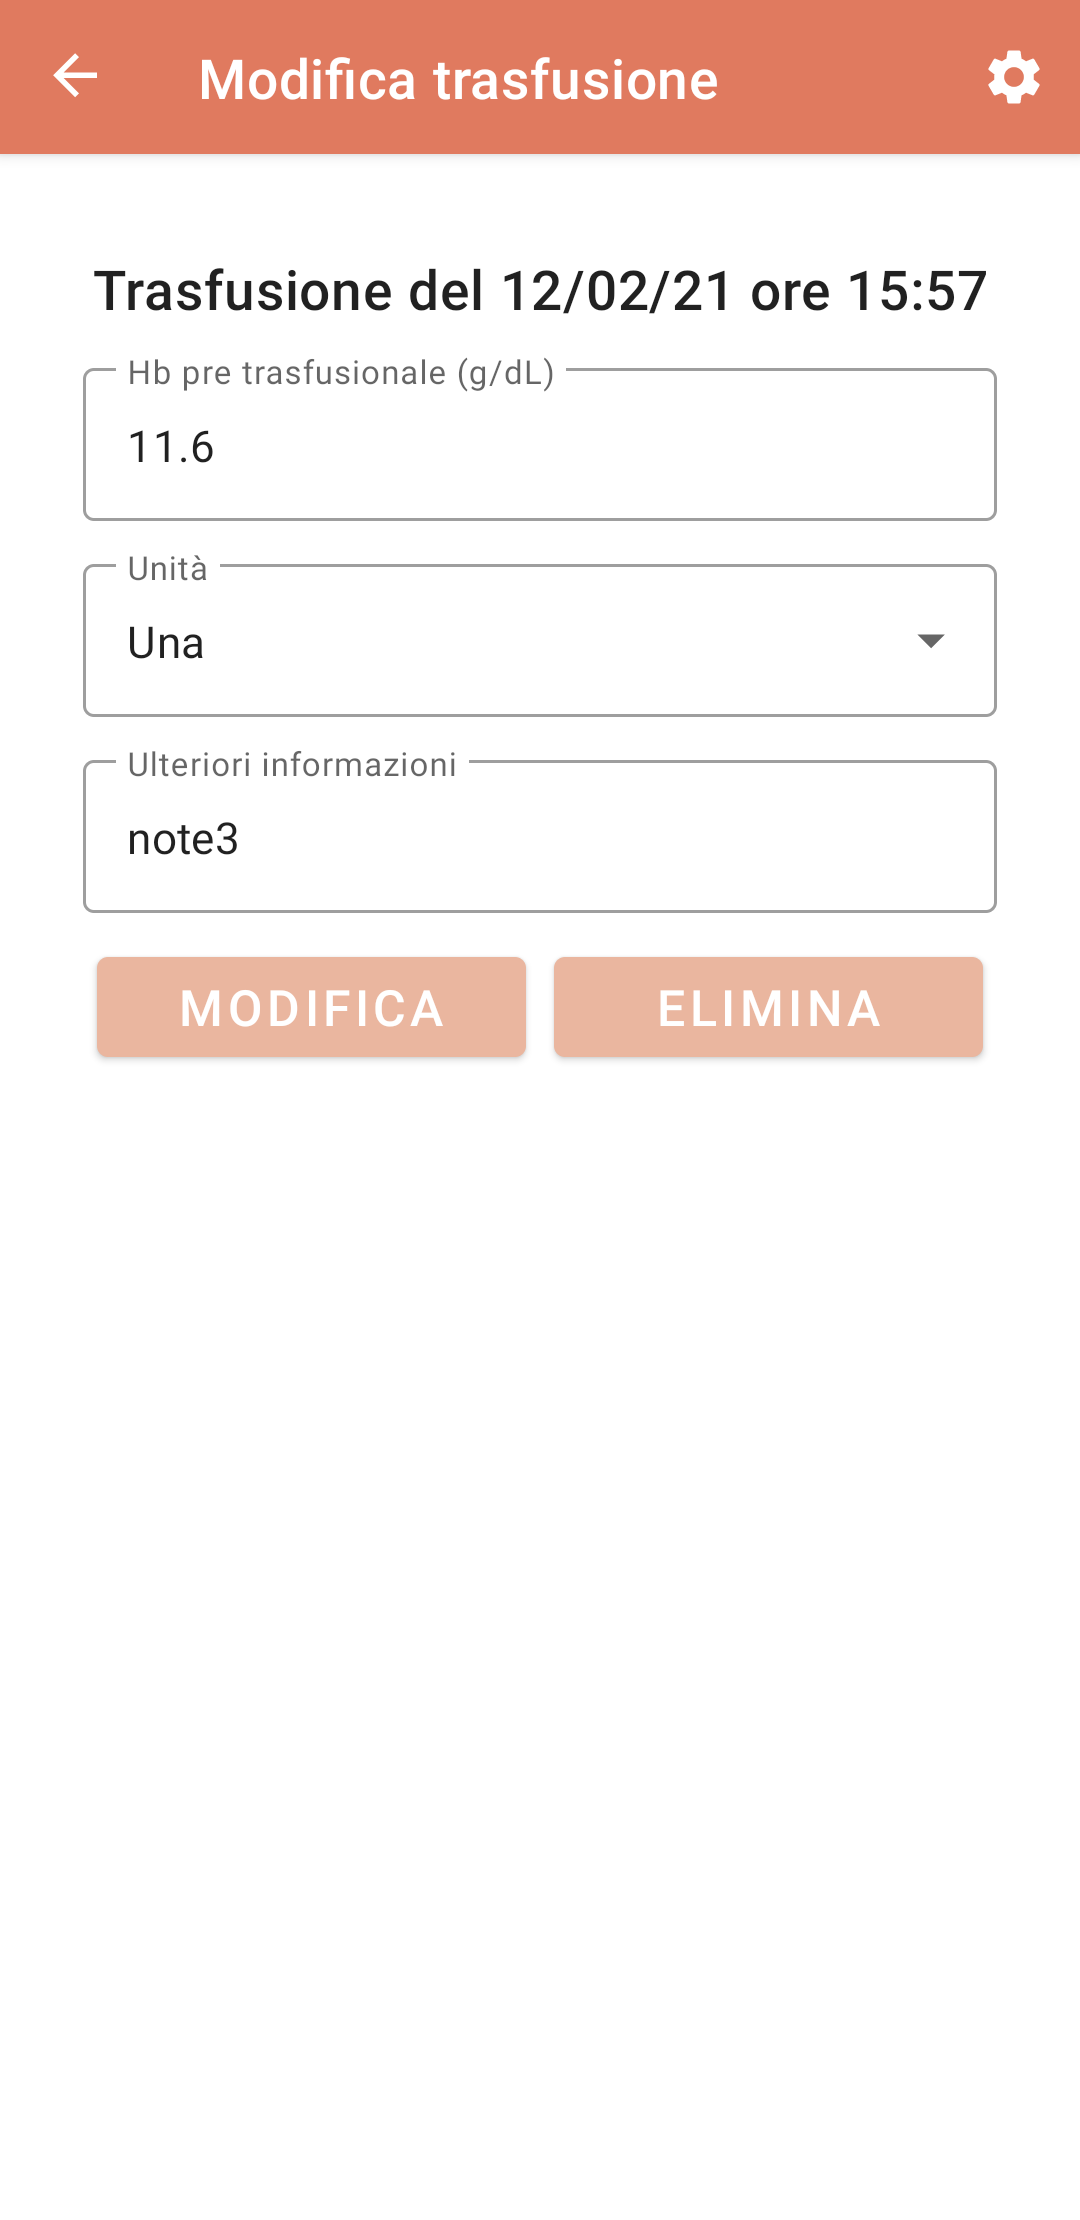
\includegraphics[width=.3\textwidth]{img/Screenshots/Trasfusioni/Modifica.png} \label{trasfusioni1B}} \quad
\subfloat[][\emph{Cronologia}]
{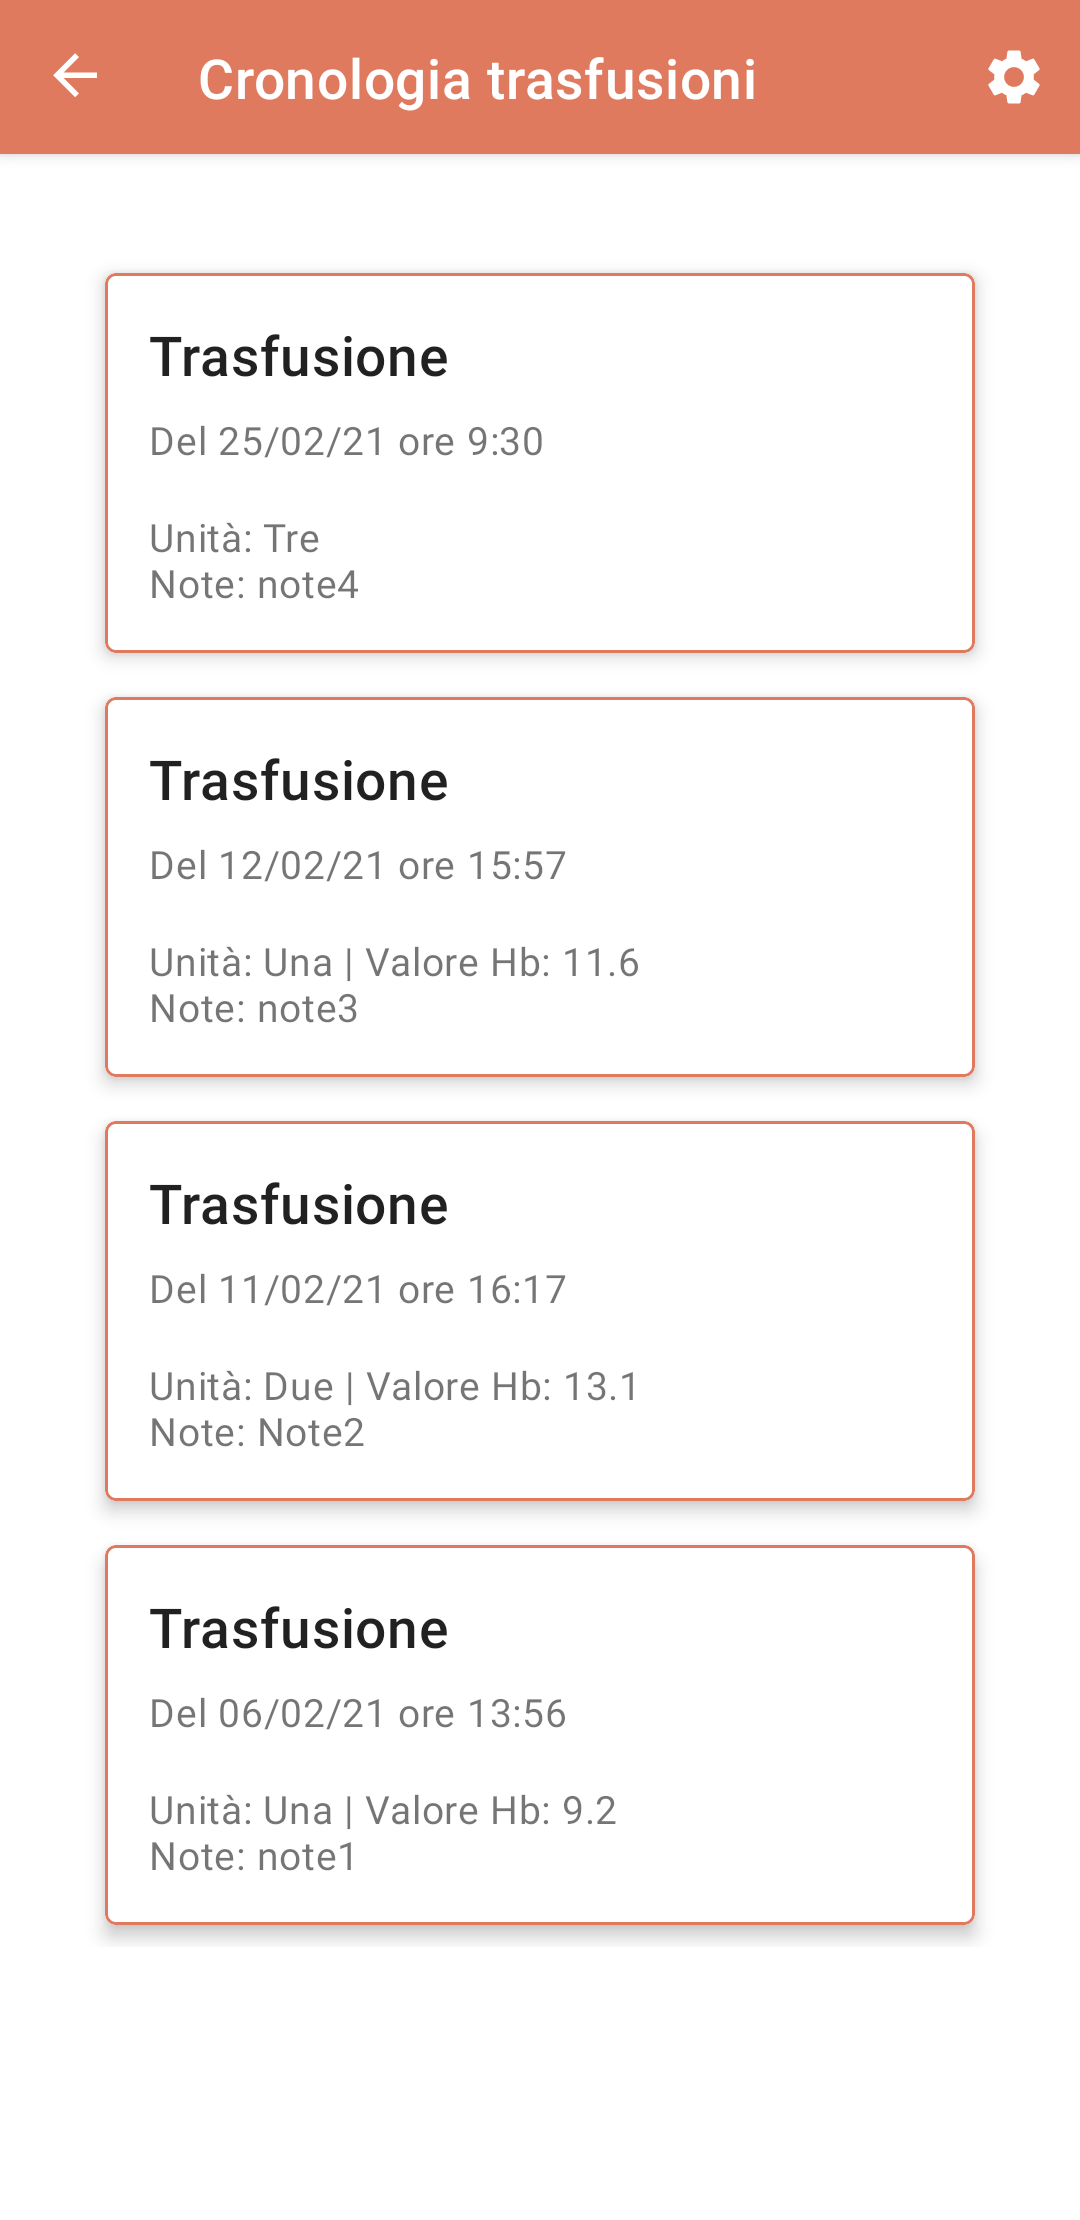
\includegraphics[width=.3\textwidth]{img/Screenshots/Trasfusioni/Cronologia.png} \label{trasfusioni1C}} \quad
\caption{Funzionalità riguardanti le trasfusioni}
\label{trasfusioni1}
\end{figure}

%Fragment1
%Fragment2
%Aggiungi
%Modifica
%Elimina
%Cronologia

\subsection{Esami e allegati}
La visualizzazione degli esami è divisa in due schermate [Fig. \ref{esamiN}] intercambiabili tramite il menù in alto, La separazione è giustificata da una gestione ottimale delle due tipologie di esami: strumentali e di laboratorio. Gli esami di laboratorio sono nella maggior parte dei casi più frequenti, mentre quelli strumentali, più radi, richiedono il più delle volte che il paziente vada fuori dal reparto trasfusionale. 

La visualizzazione della scheda esame cambia in base alla presenza o meno di allegati di riferimento. In figura \ref{esamiM} è mostrato un esame e in figura \ref{esamiA} lo stesso con un allegato.

Il funzionamento delle componenti della schermata rimane in linea con quello descritto nelle trasfusioni: il pulsante in alto permette l'aggiunta di esami di entrambe le tipologie; se presenti esami futuri vengono visualizzati di seguito; se presenti esami passati appaiono nel layout le componenti per aggiungere dati e visualizzare la cronologia della stessa tipologia d'esame.

%FragmentLaboratorio
%FragmentStrumentali

\begin{figure}[H]
\centering
\subfloat[][\emph{Esami di laboratorio}]
{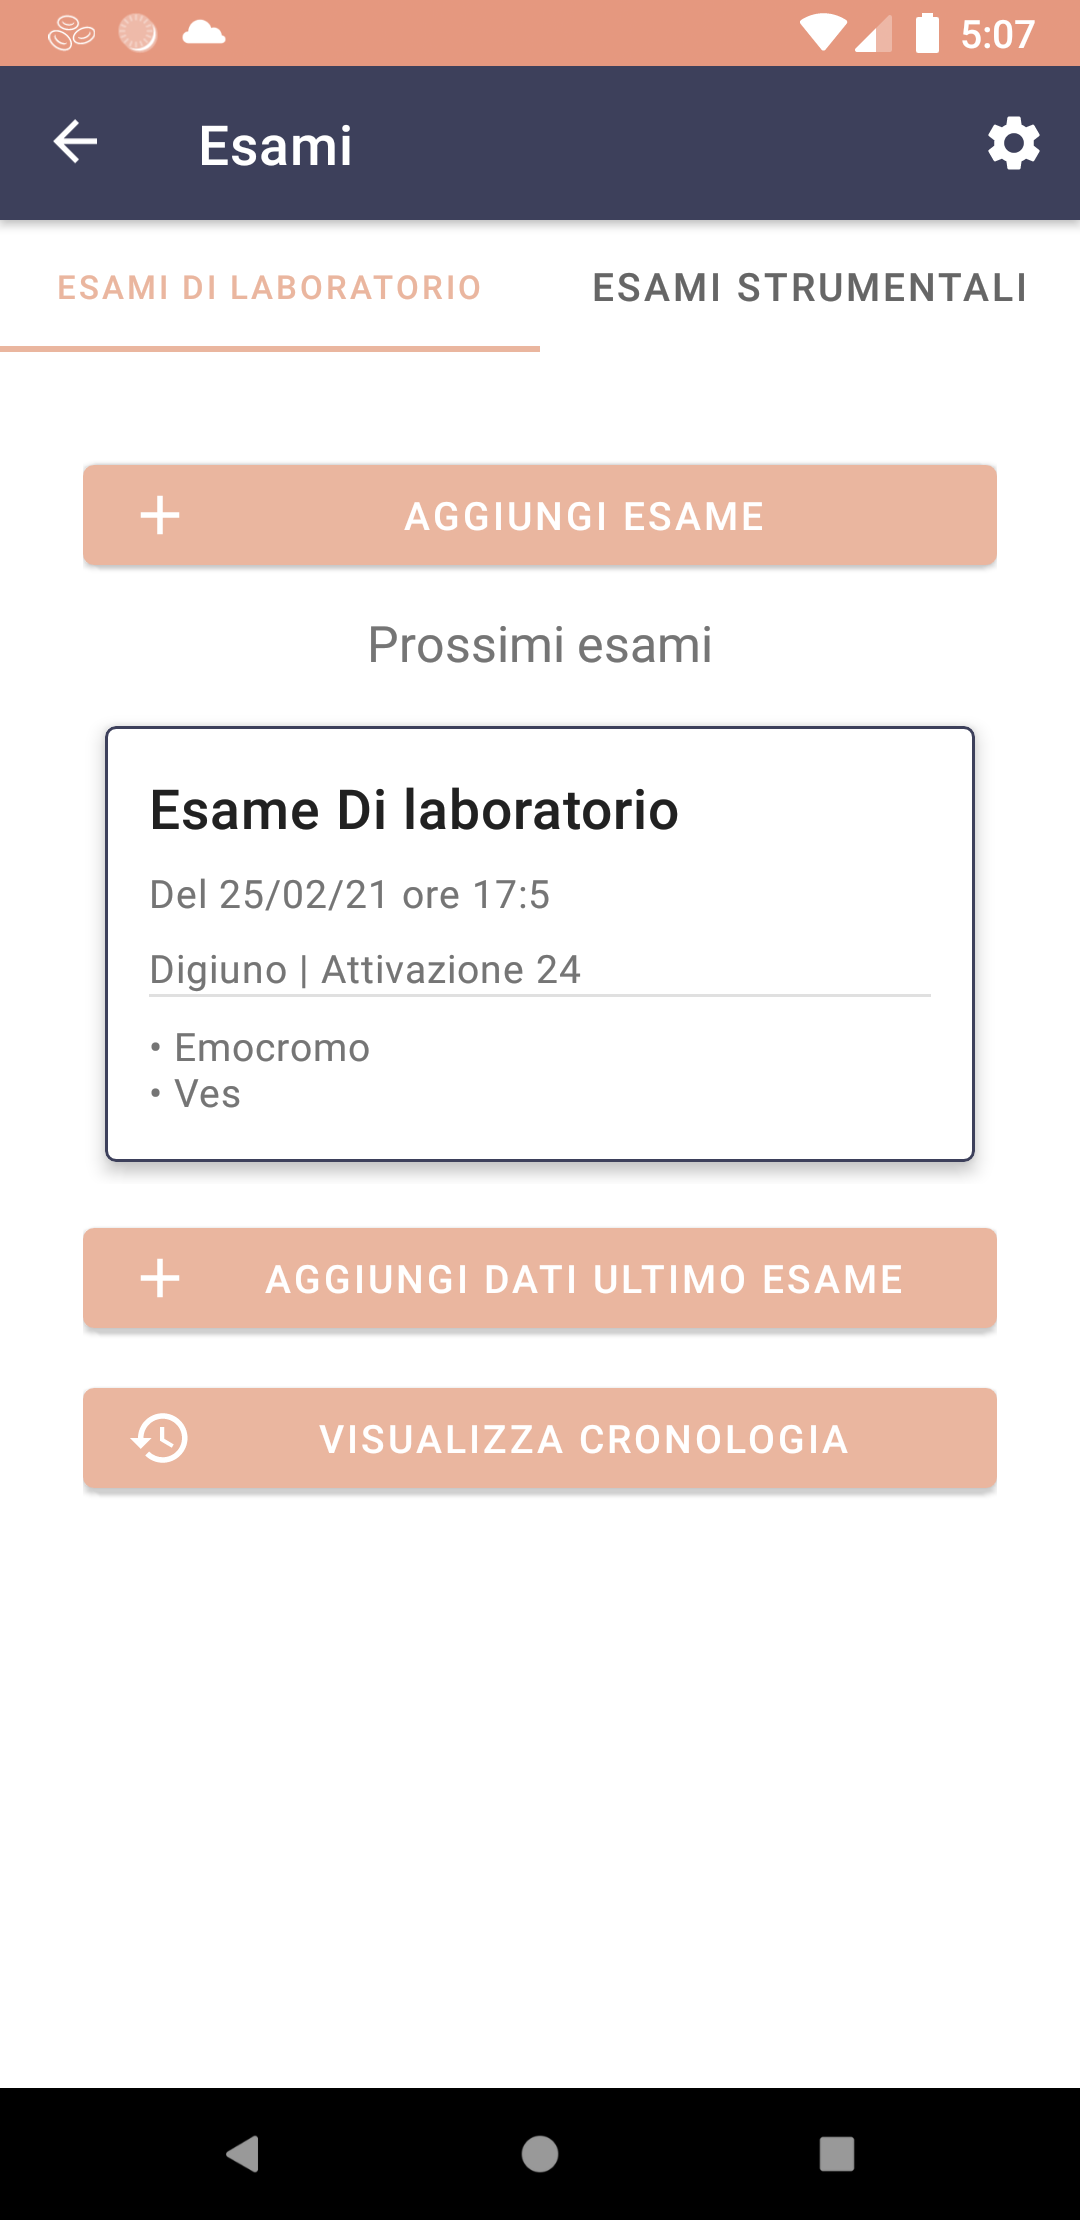
\includegraphics[width=.3\textwidth]{img/Screenshots/Esami/FragmentLaboratorio.png} \label{esamiA}} \quad
\subfloat[][\emph{Esami strumentali}]
{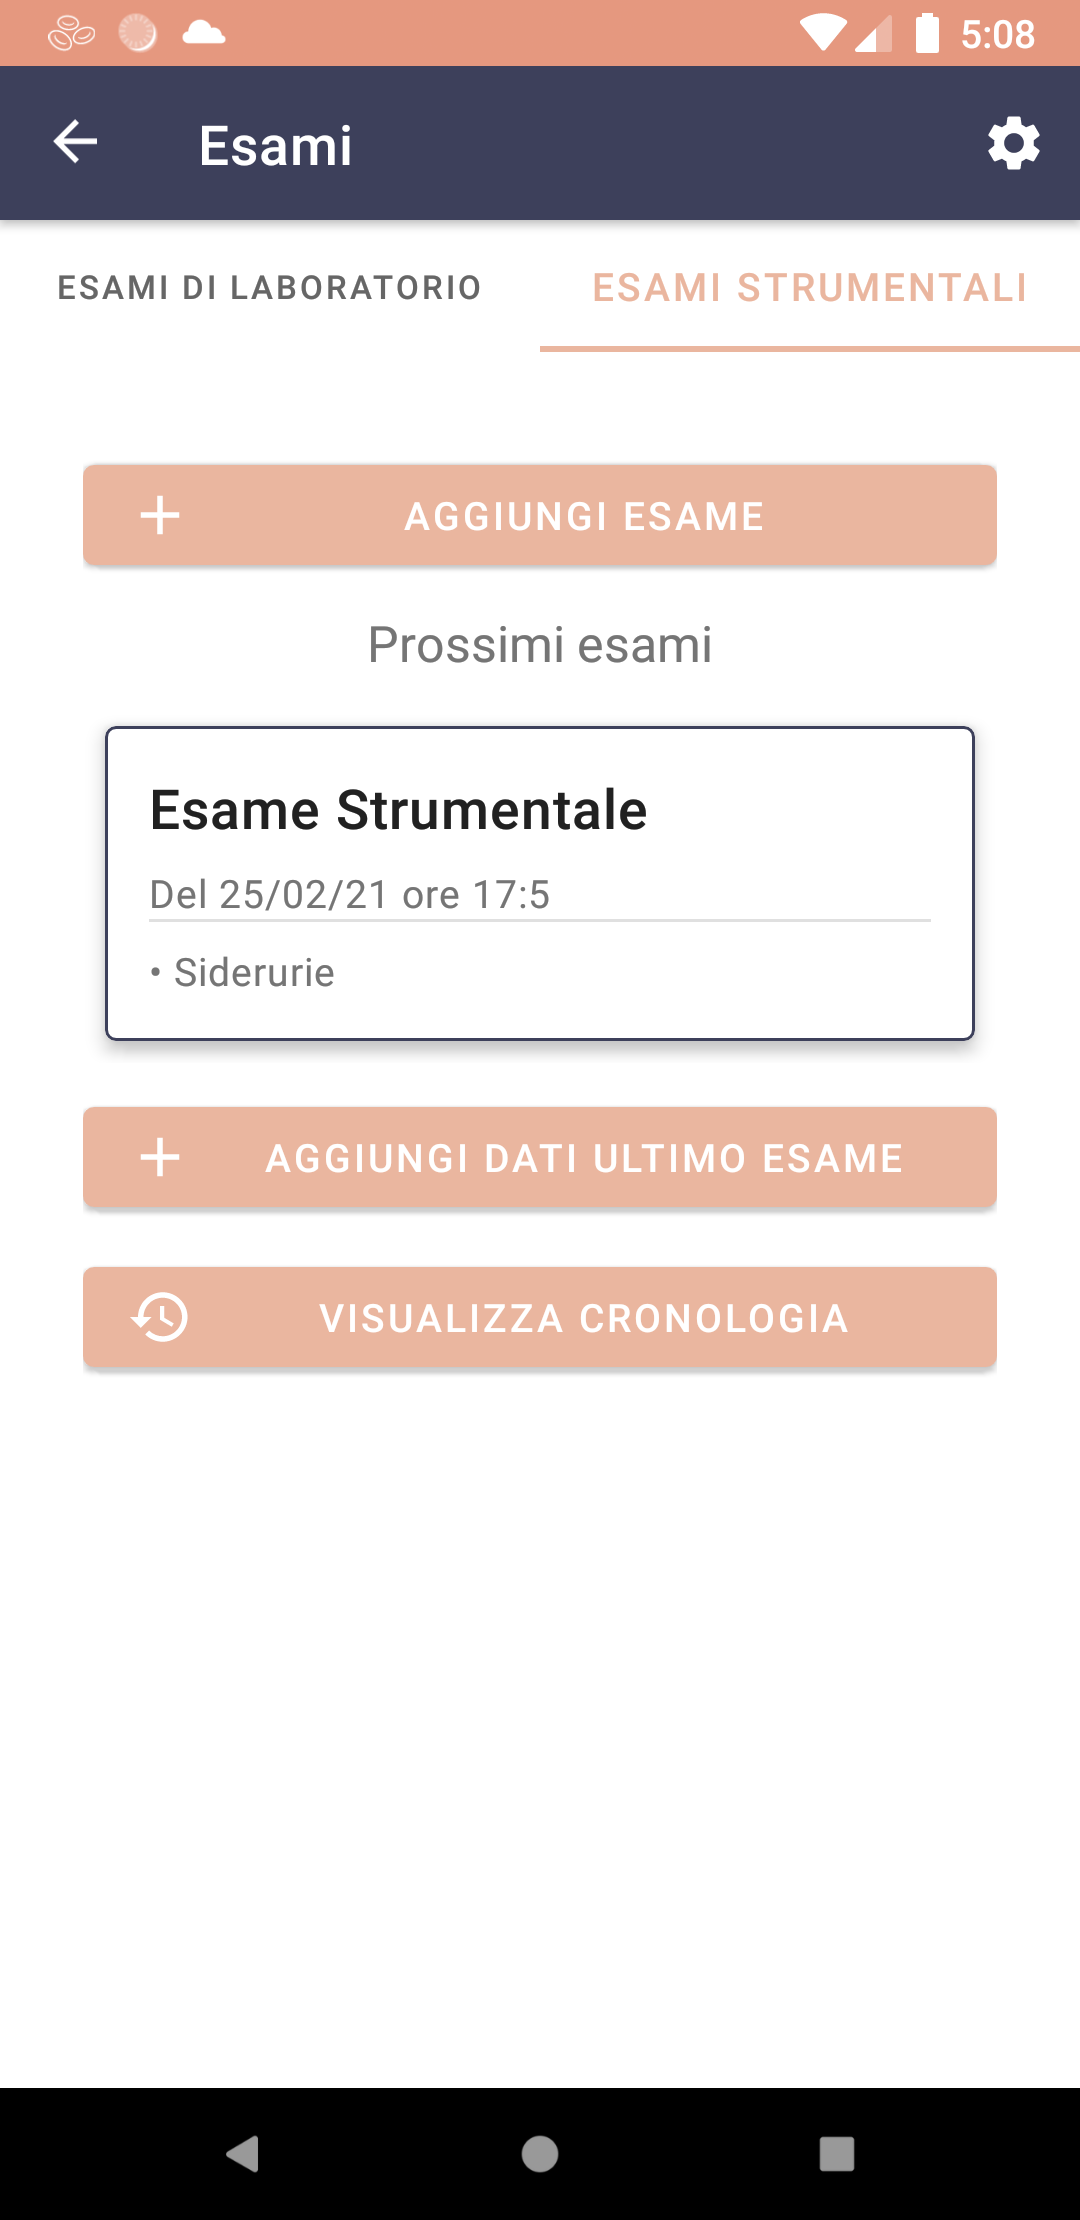
\includegraphics[width=.3\textwidth]{img/Screenshots/Esami/FragmentStrumentali.png} \label{esamiB}} \quad
\subfloat[][\emph{Esame con anteprima allegato}]
{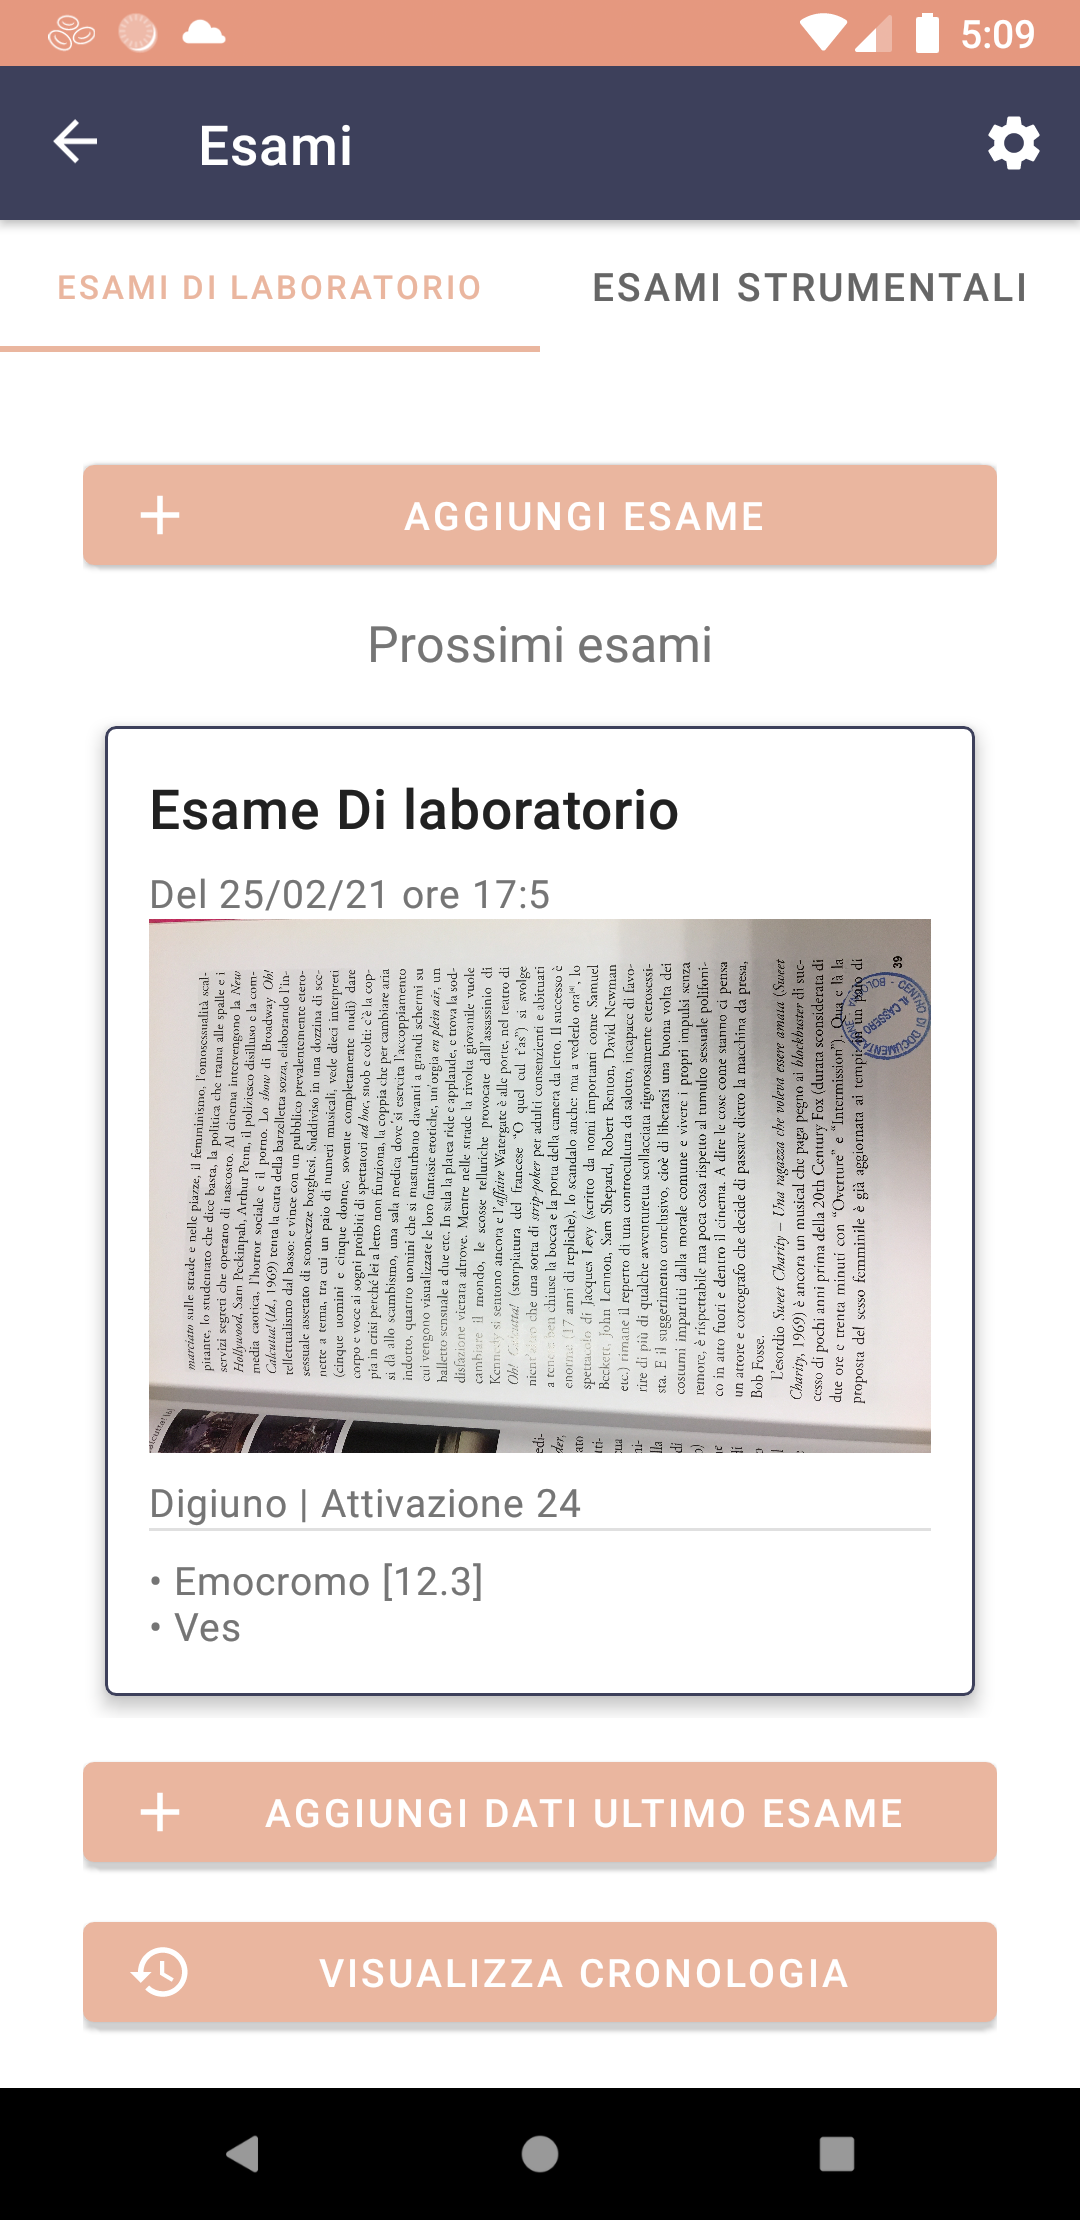
\includegraphics[width=.3\textwidth]{img/Screenshots/Esami/FragmentConAllegato.png} \label{esamiM}} \quad
\caption{Schermata dedicata agli esami}
\label{esamiN}
\end{figure}


La modalità di aggiunta degli esami varia in base alla sua tipologia:
\begin{itemize}
    \item Esami di laboratorio [Fig. \ref{esamiC}]: è obbligatorio inserire un nome, una data, un orario e un'analisi. Le analisi racchiudono dati concreti dell'esame stesso, motivo per cui deve esserne presente almeno una. \`E a discrezione dell'utente attivare o meno la spunta del digiuno e quella dell'attivazione anticipata.
    \item Esami strumentali [Fig. \ref{esamiD}]: è obbligatorio inserire un nome, una data e un orario. Il nome dell'esame fa riferimento ai dati che contiene e non sono presenti analisi specifiche. Le funzionalità per il digiuno e per l'attivazione anticipata rimangono le stesse.
\end{itemize}

La cronologia [Fig. \ref{esamiE}] mostra solo gli esami della tipologia selezionata.

%AggiungiDiLaboratorio
%AggiungiStrumentali
%Cronologia
\begin{figure}[H]
\centering
\subfloat[][\emph{Aggiunta esami di laboratorio}]
{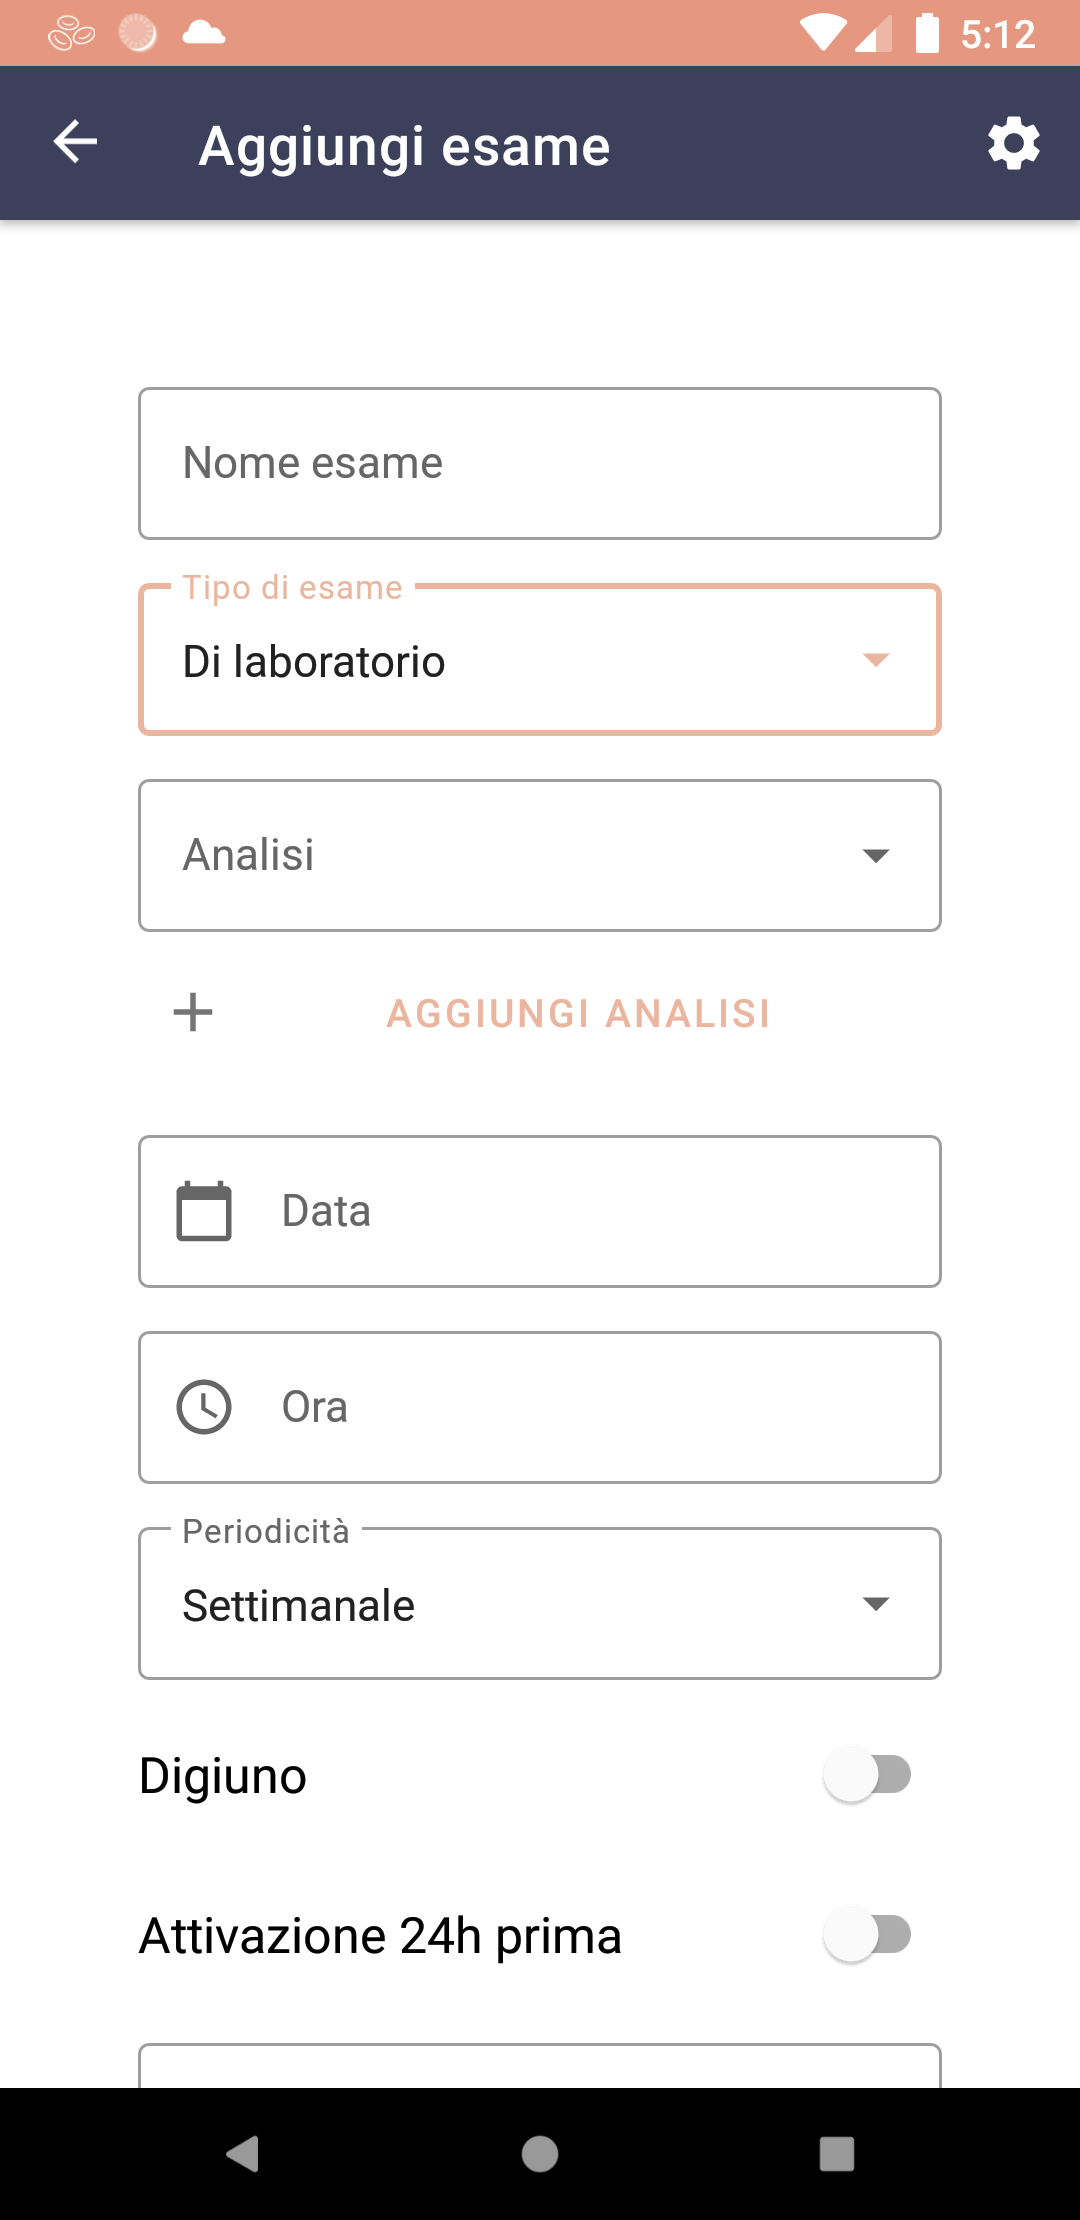
\includegraphics[width=.3\textwidth]{img/Screenshots/Esami/AggiungiDiLaboratorio.png} \label{esamiC}} \quad
\subfloat[][\emph{aggiunta esami strumentali}]
{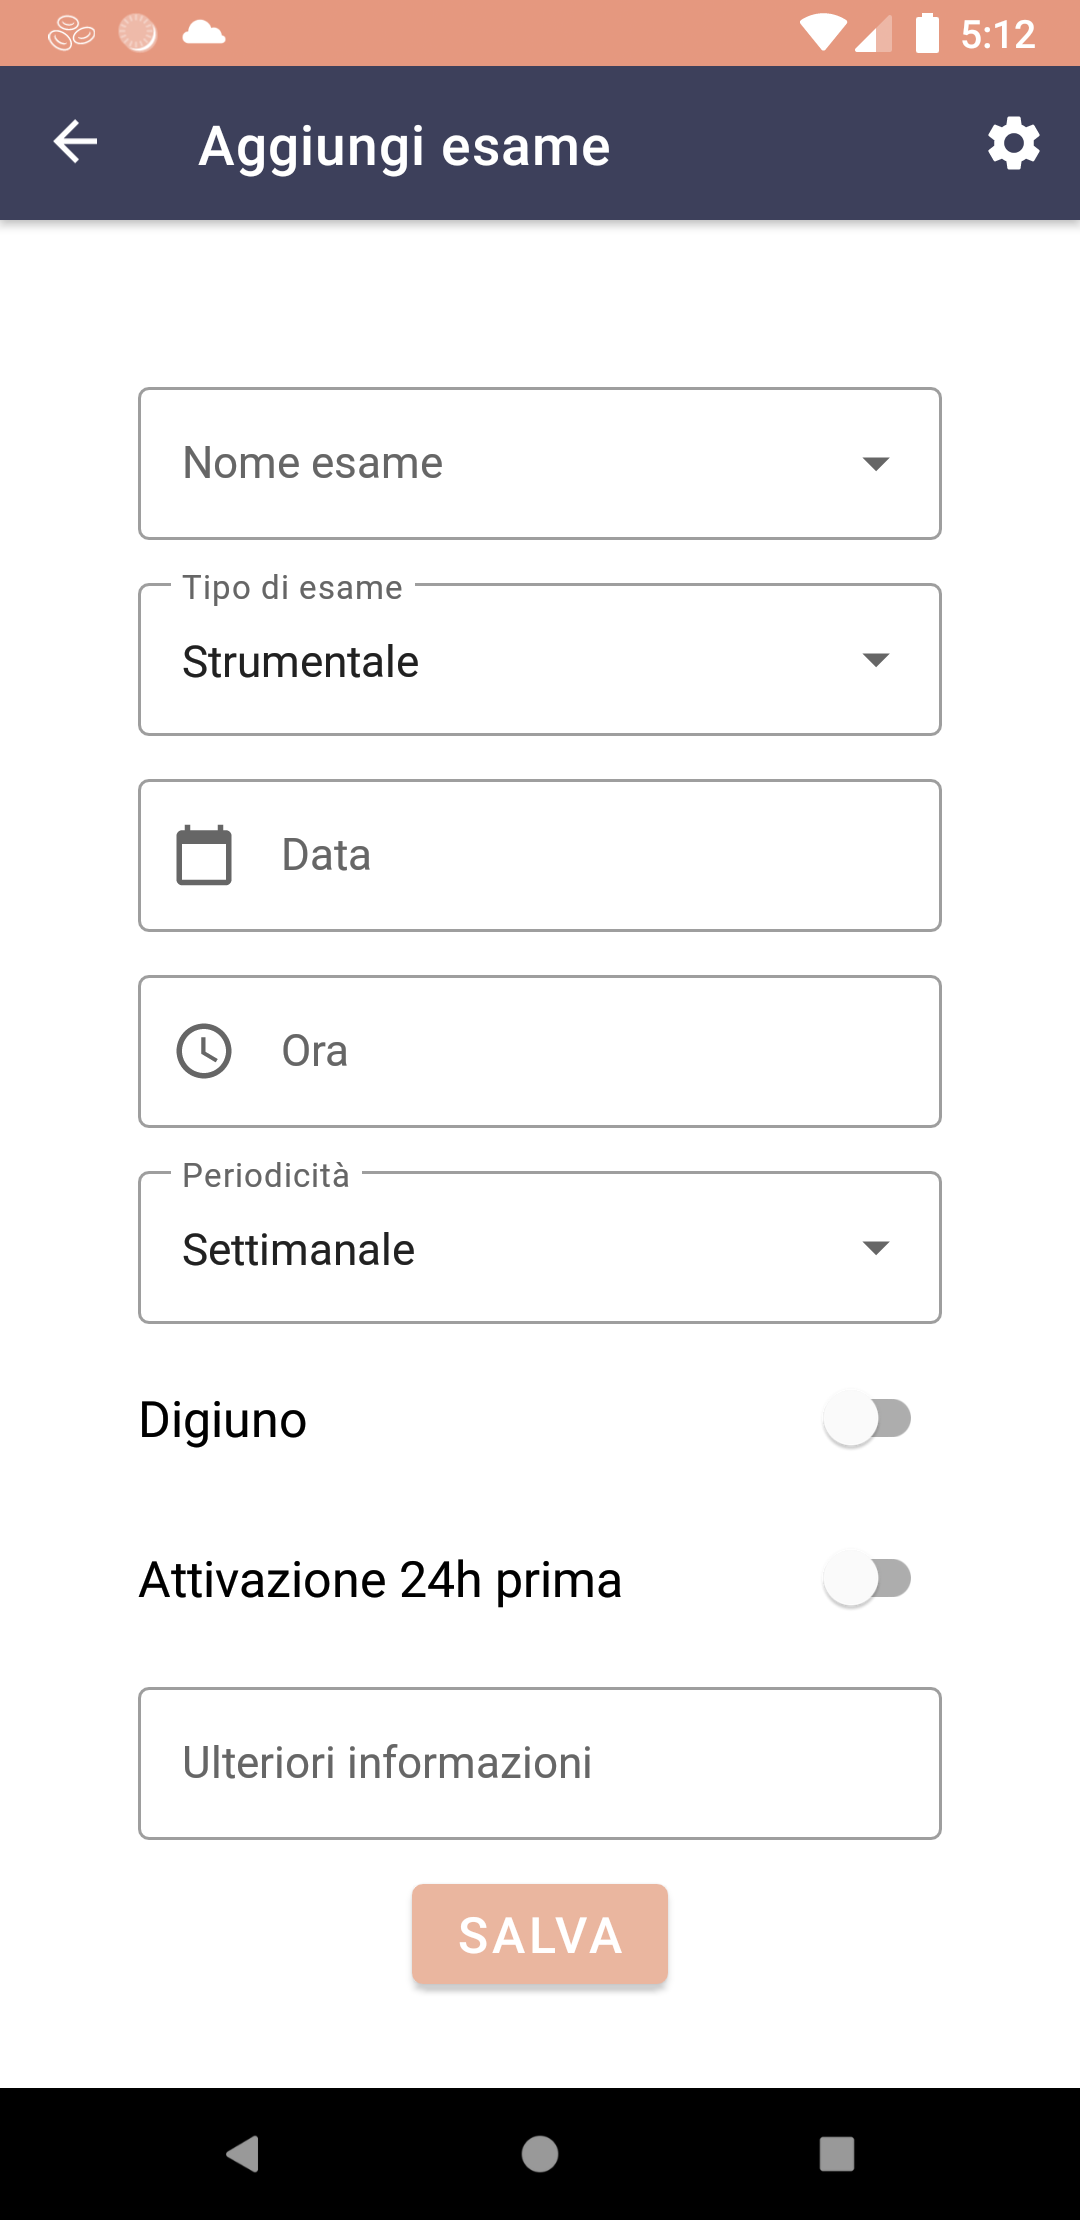
\includegraphics[width=.3\textwidth]{img/Screenshots/Esami/AggiungiStrumentale.png} \label{esamiD}} \quad
\subfloat[][\emph{Cronologia}]
{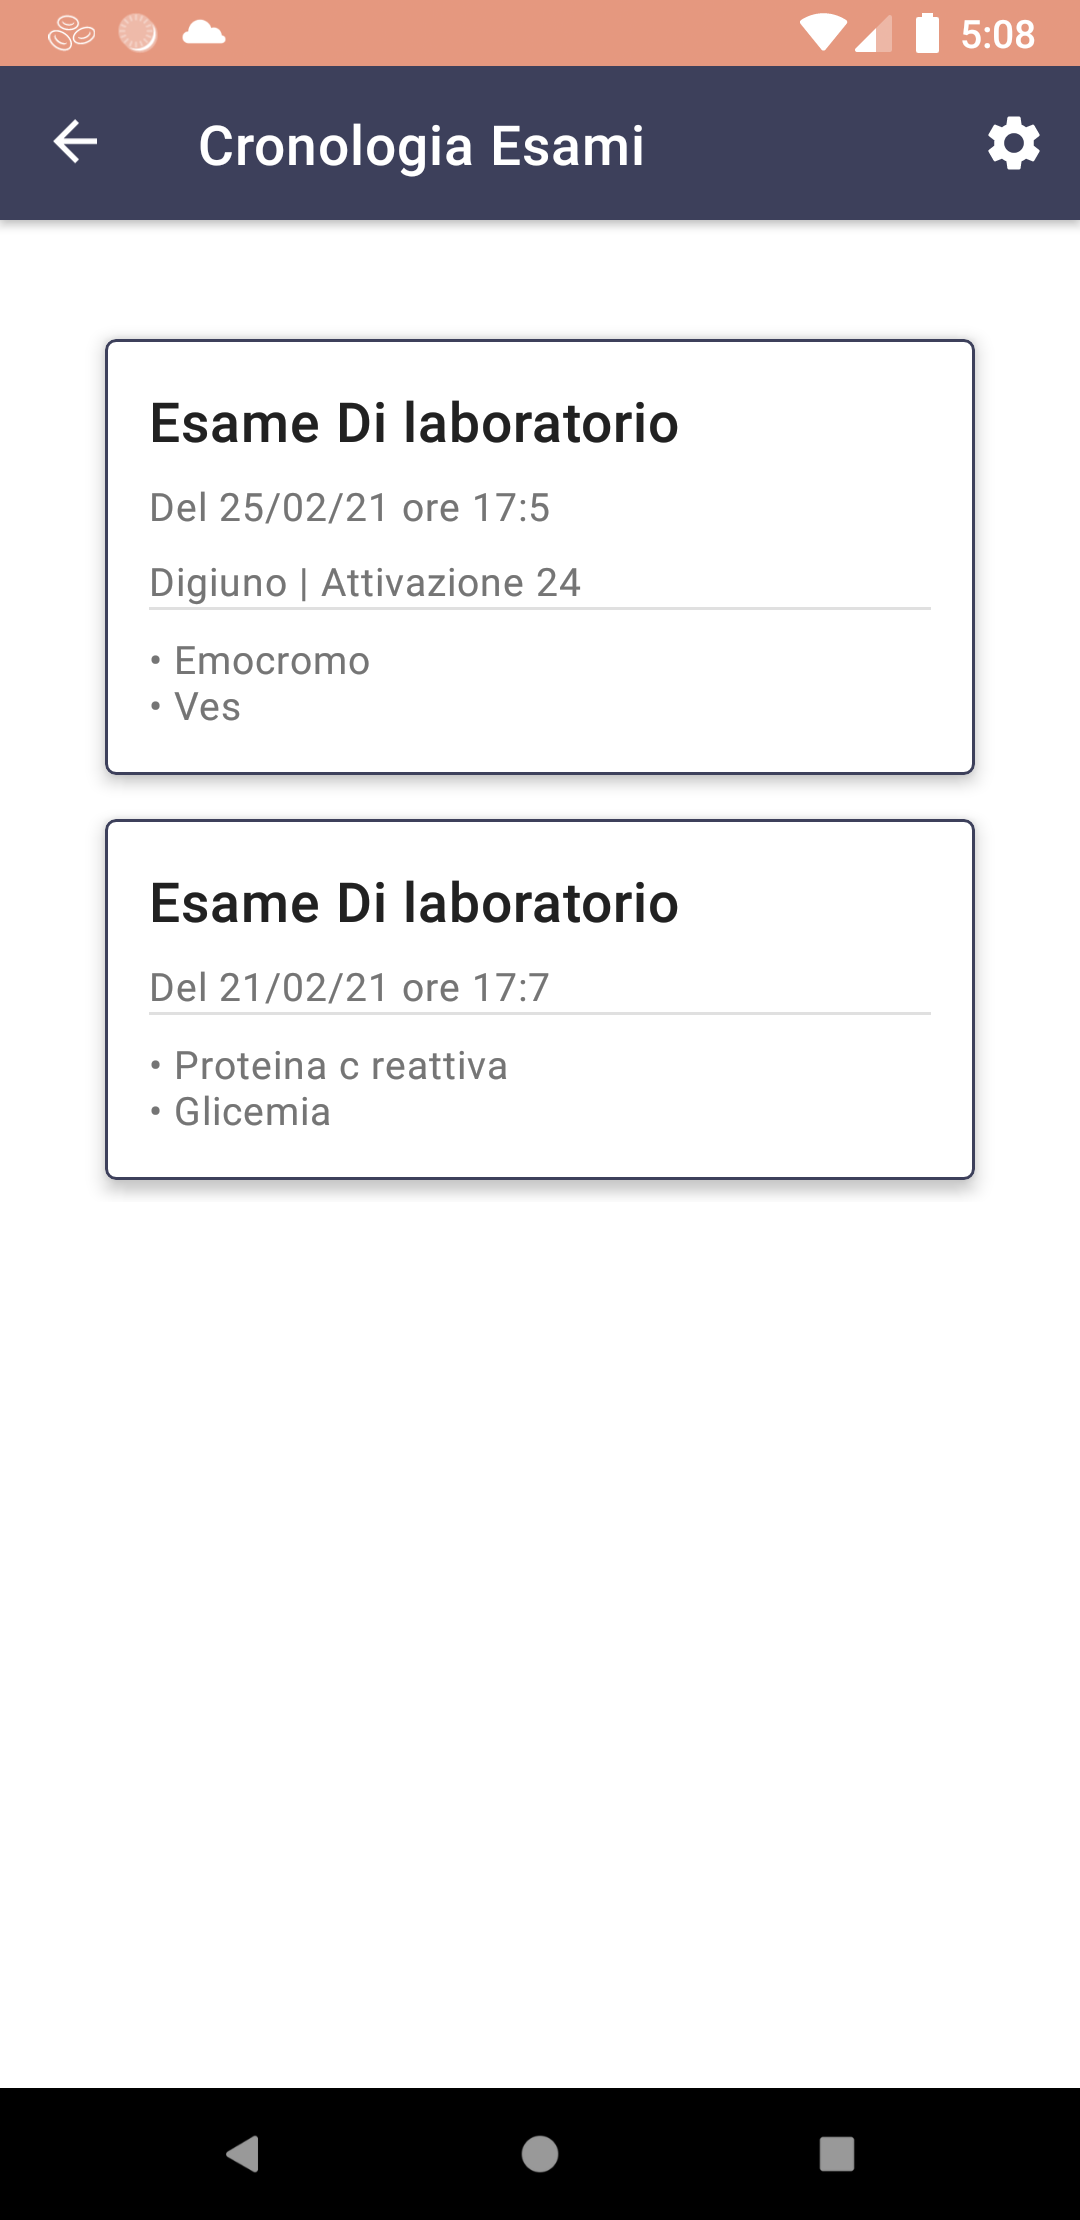
\includegraphics[width=.3\textwidth]{img/Screenshots/Esami/Cronologia.png} \label{esamiE}} \quad
\caption{Funzionalità riguardanti gli esami}
\label{esamiF}
\end{figure}

\subsubsection{Allegati}
Gli allegati si possono aggiungere dalla schermata di modifica esame e se ne possono inserire un massimo di 3 alla volta.
Quando si carica un file come allegato, appare una piccola immagine di riferimento [Fig. \ref{esamiG}]. Per inviare definitivamente il file nel database bisogna sfruttare la componente di caricamento degli allegati, solo in seguito le immagini caricate occupano l'intero schermo in lista [Fig. \ref{esamiH}]. La componente che raffigura un secchio dell'immondizia serve ad eliminare l'allegato.
Toccando un elemento allegato viene visualizzato singolarmente a tutto schermo [Fig. \ref{esamiI}].

%UploadAllegato
%ModificaConAllegato
%MostraAllegato

\begin{figure}[H]
\centering
\subfloat[][\emph{Upload degli allegati}]
{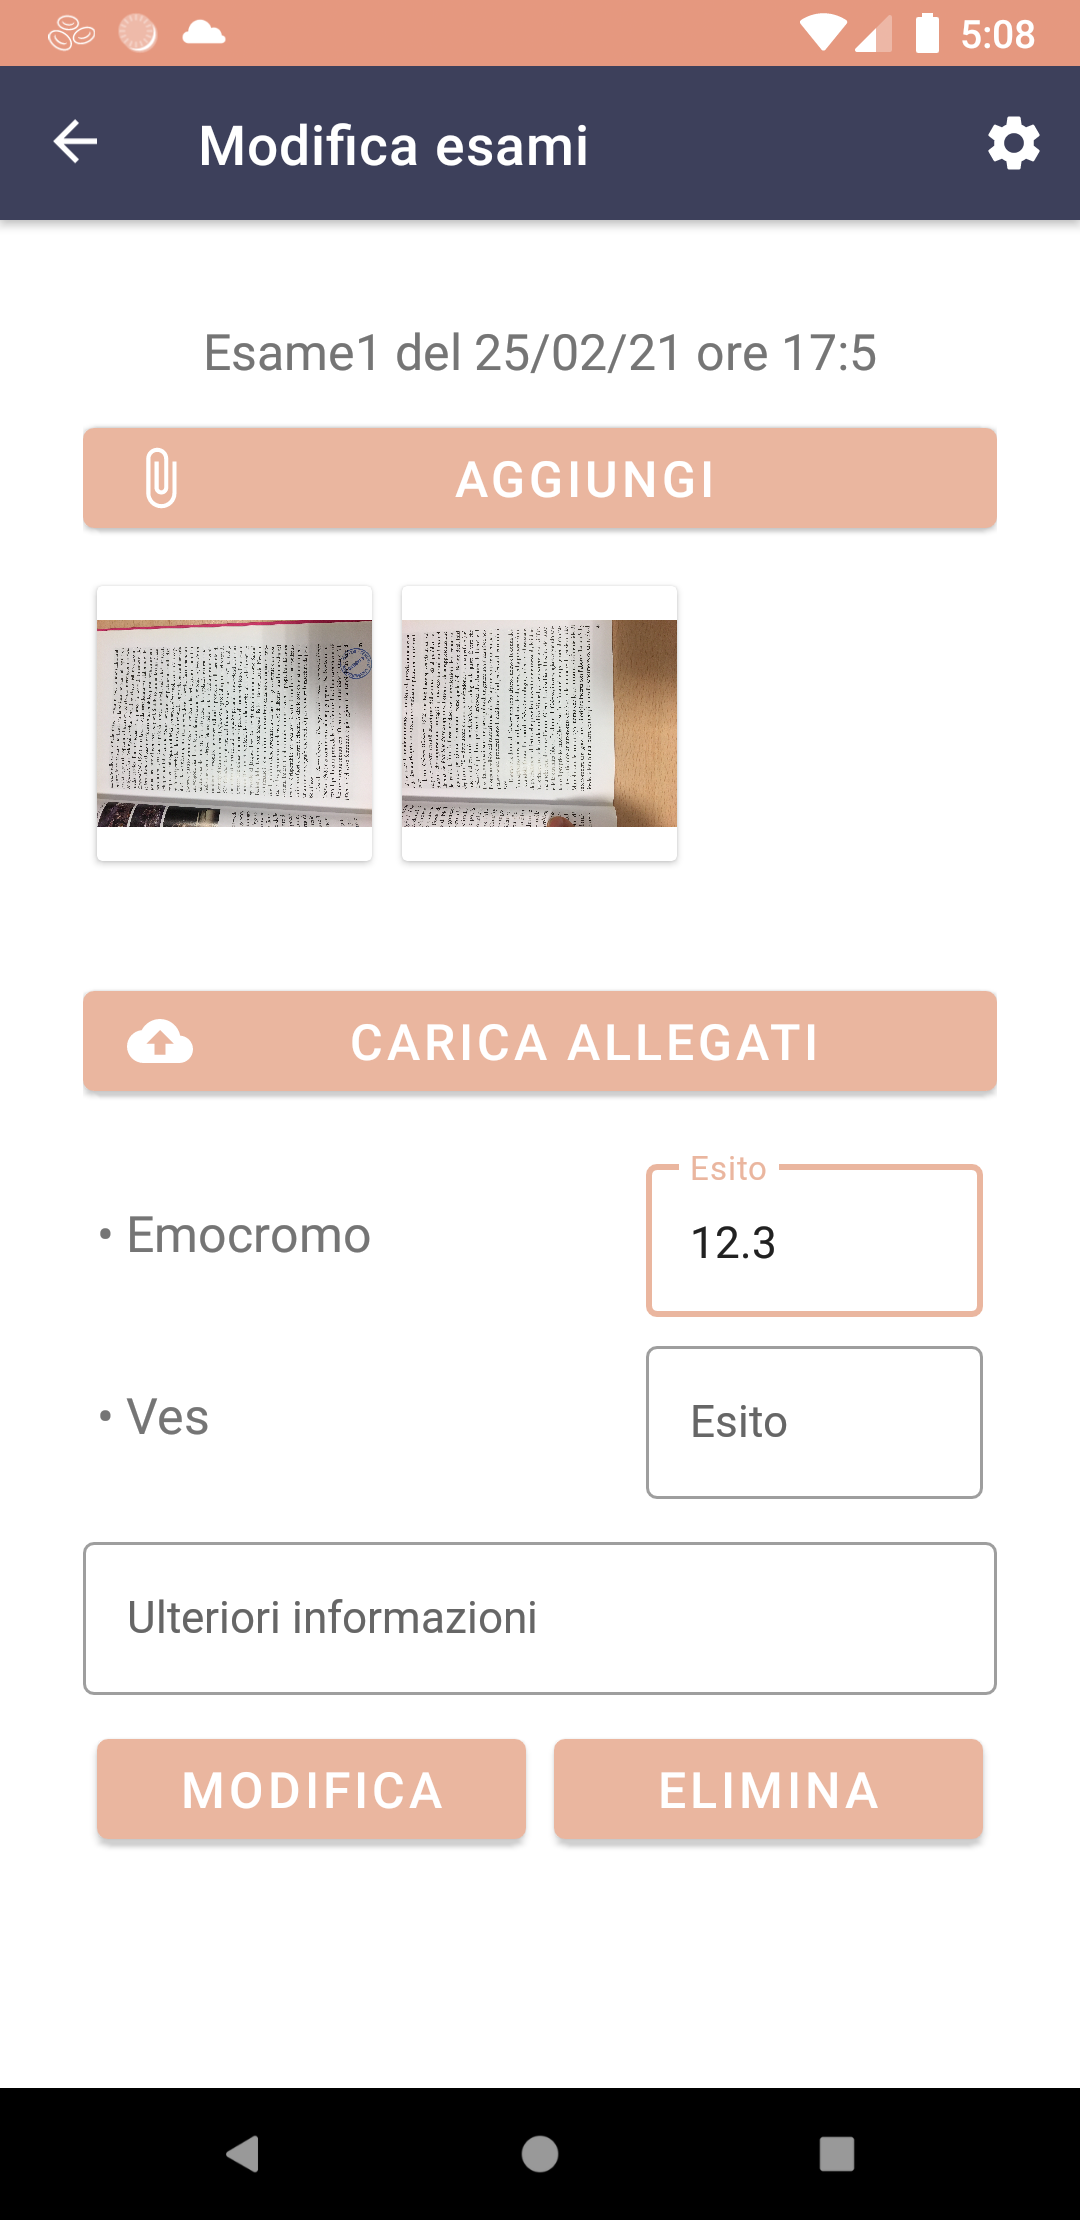
\includegraphics[width=.3\textwidth]{img/Screenshots/Esami/UploadAllegati.png} \label{esamiG}} \quad
\subfloat[][\emph{Visualizzazione scheda esame con allegato}]
{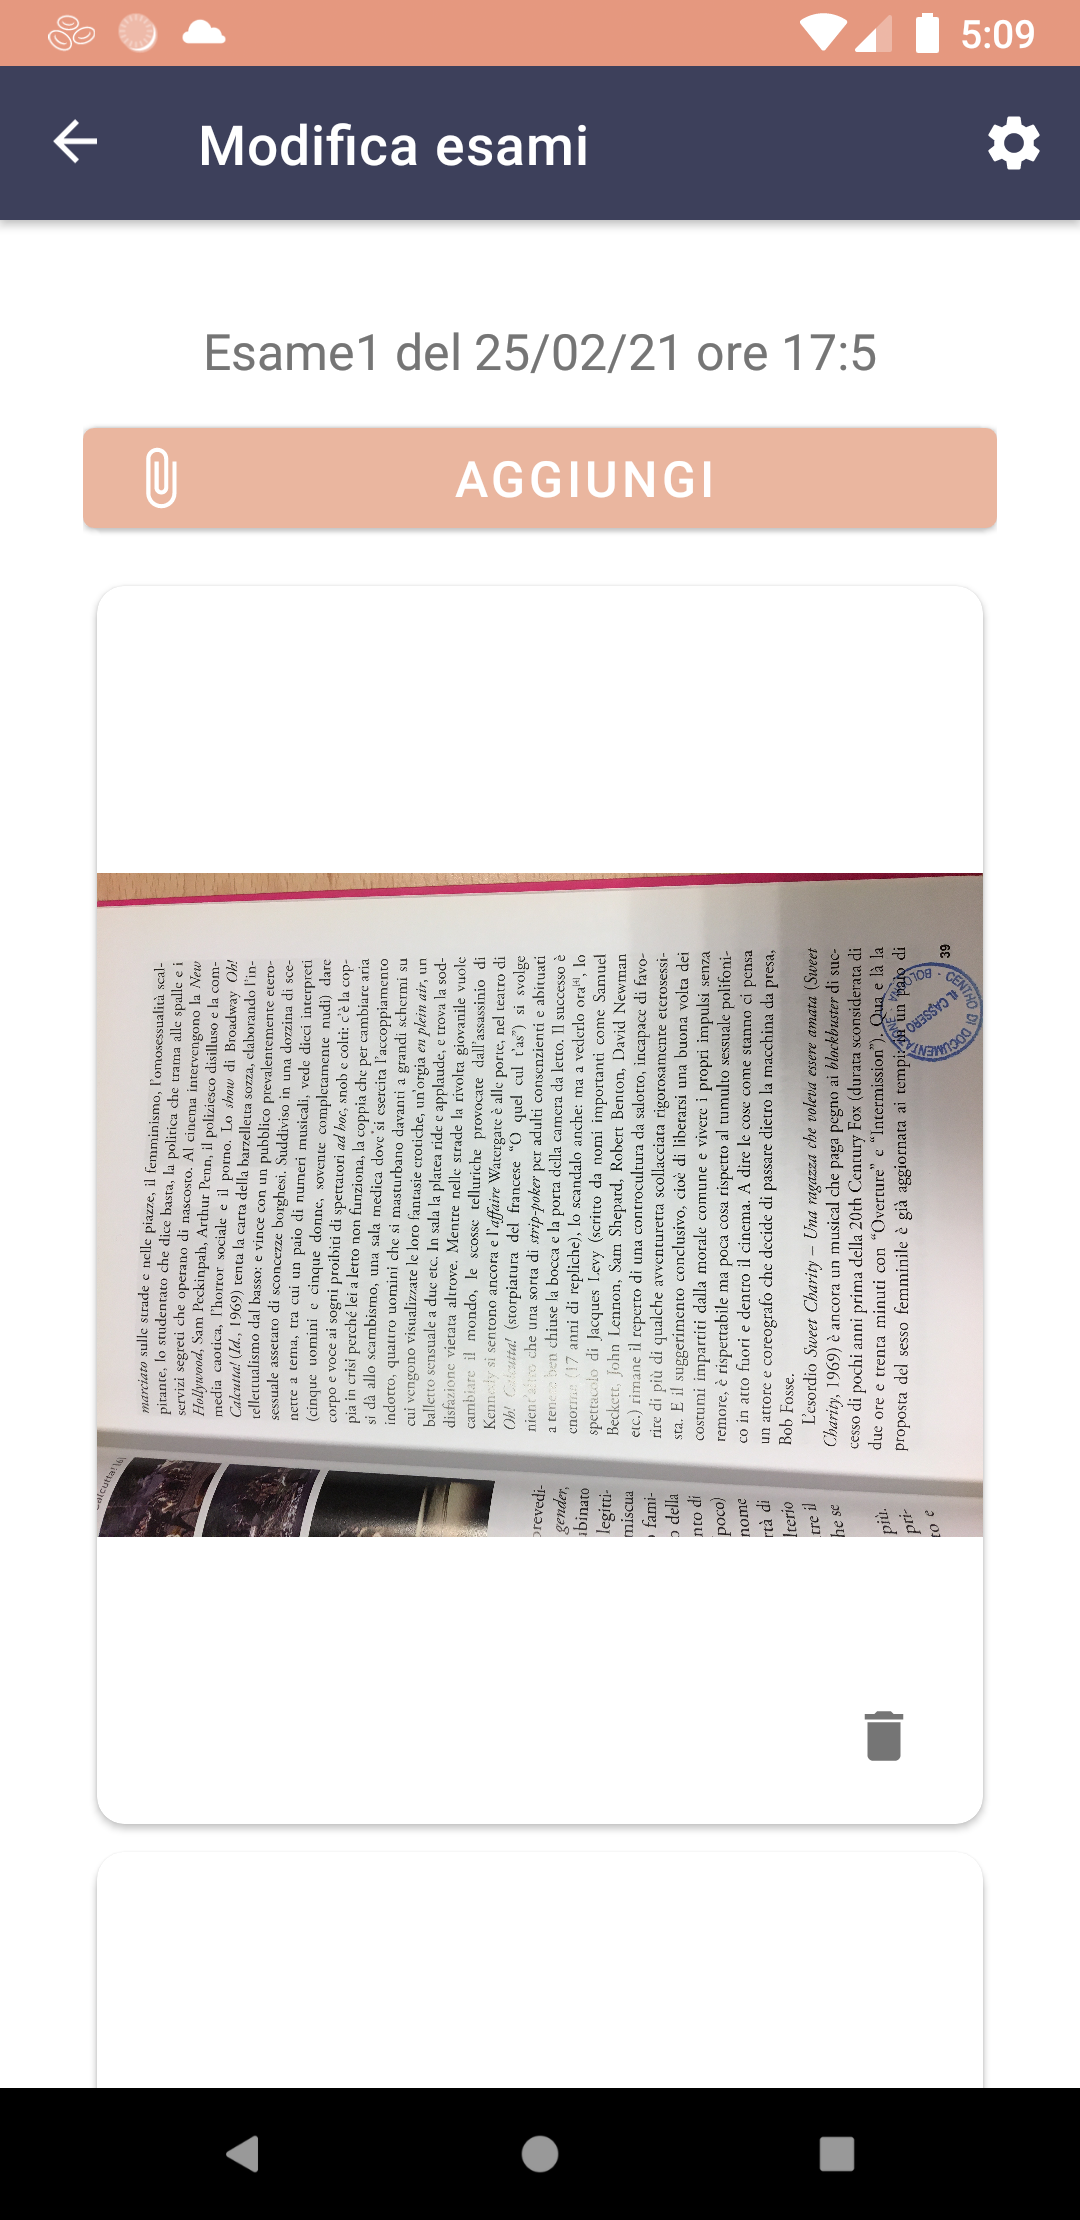
\includegraphics[width=.3\textwidth]{img/Screenshots/Esami/ModificaConAllegato.png} \label{esamiH}} \quad
\subfloat[][\emph{Schermata di visualizzazione singolo allegato}]
{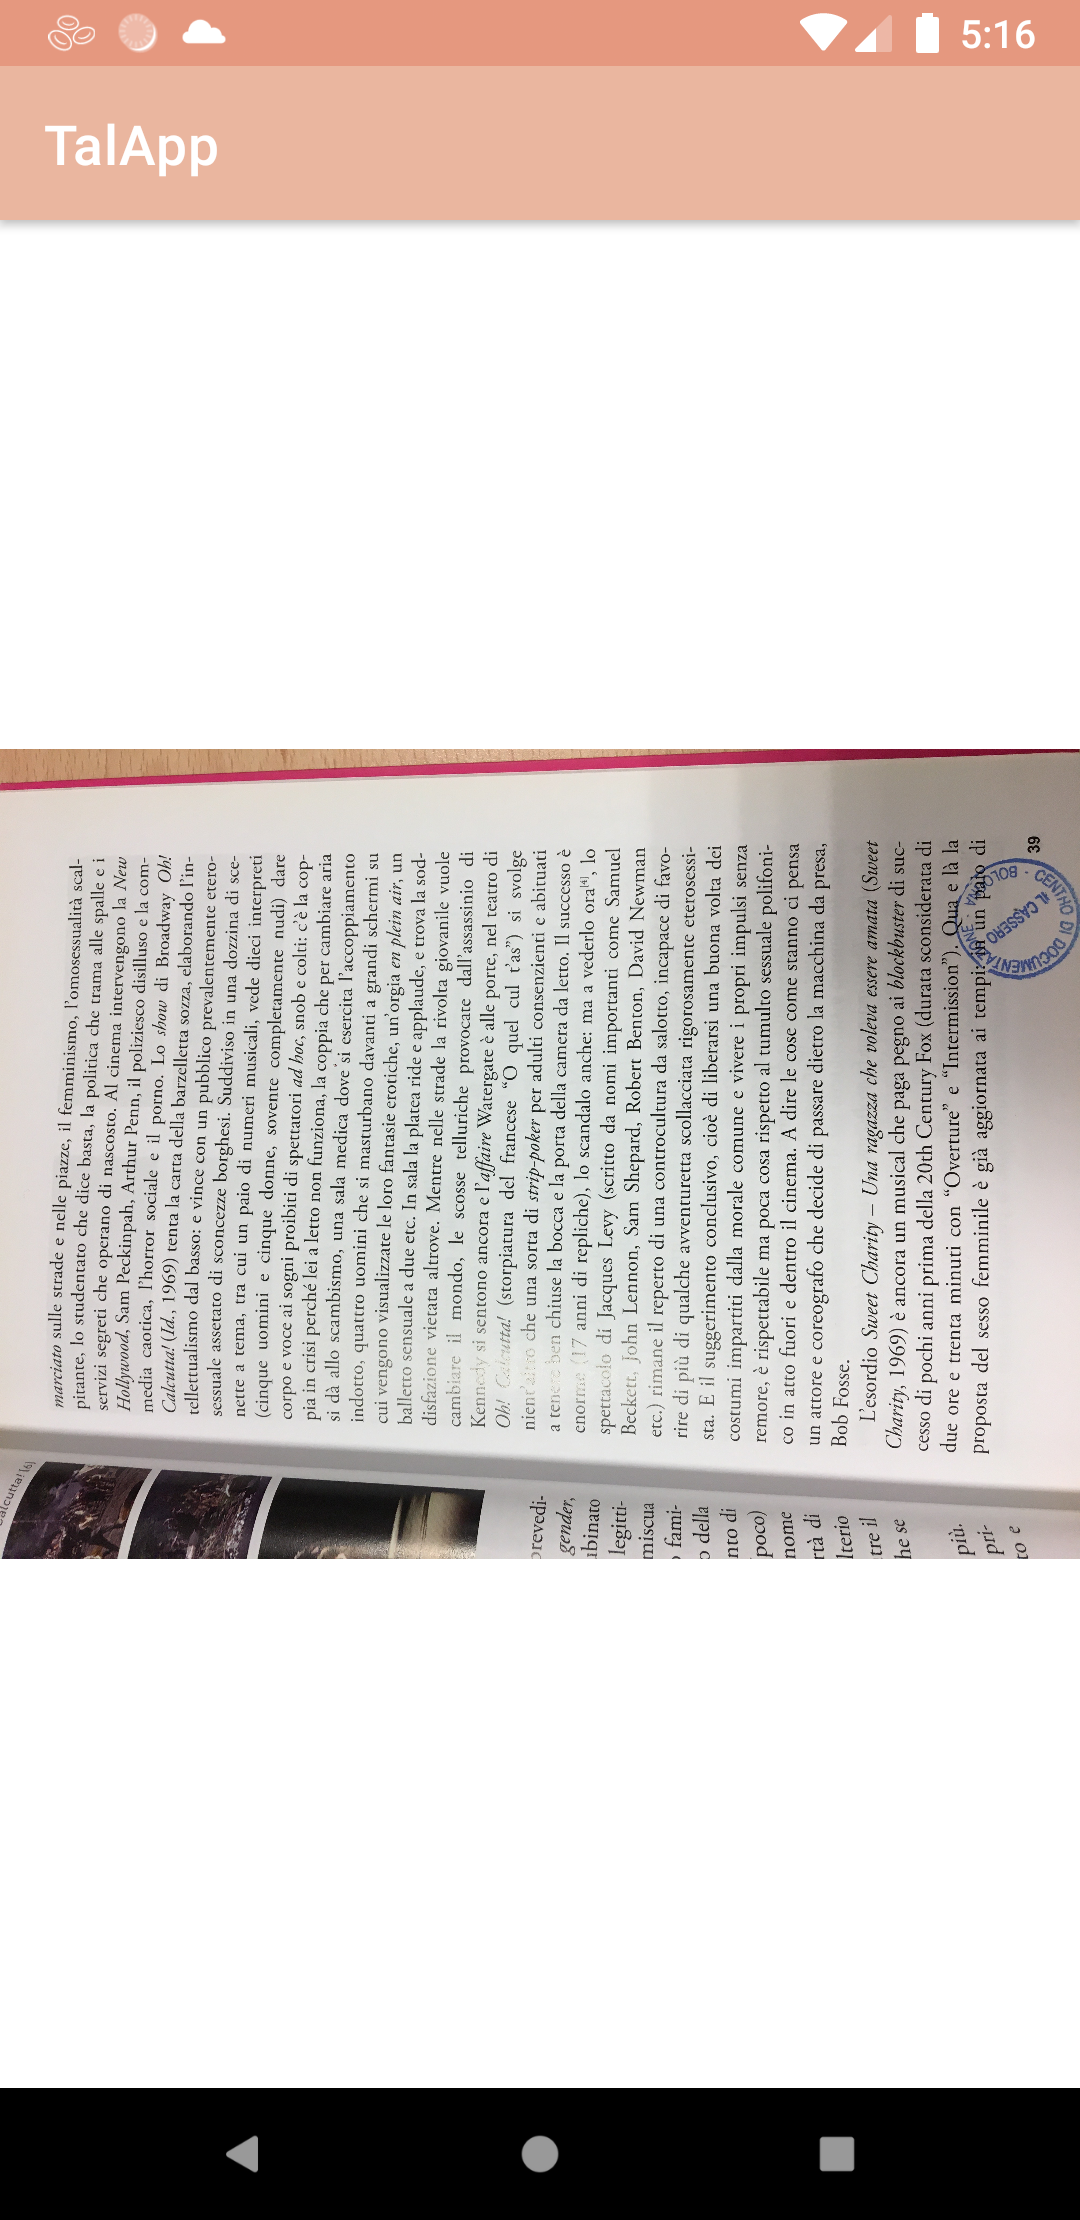
\includegraphics[width=.3\textwidth]{img/Screenshots/Esami/MostraAllegato.png} \label{esamiI}} \quad
\caption{Funzionalità riguardanti gli allegati}
\label{esamiL}
\end{figure}

\subsection{Terapie e sveglie}
La schermata delle terapie è accessibile dalla home e le sue funzionalità sono nel complesso le stesse delle altre due tipologie di eventi. 
In figura \ref{terapiaA} è presente la componente che per mette di aggiungere nuove terapie, la la lista delle terapie attuali e la cronologia. 

Quando si aggiunge una nuova terapia è necessario specificare un periodo di riferimento, il nome e la dose del farmaco da assumere.

\subsubsection{Sveglie}
La peculiarità di questa tipologia di evento sono le sveglie, è possibile aggiungerle in fase di inserimento [Fig. \ref{terapiaB})] e modifica [Fig. \ref{terapiaC}] di una terapia. L'aggiunta di una sveglia non ne determina l'attivazione, per impostarla bisogna selezionare uno o più giorni della settimana e toccare la levetta in alto a destra. \`E possibile rimuovere gli allarmi solo dalla schermata di modifica delle terapie, toccando sull'icona sotto la levetta di attivazione.

%Aggiungi
%Cronologia
%Fragment
\begin{figure}[H]
\centering
\subfloat[][\emph{Schermata dedicata alle terapie}]
{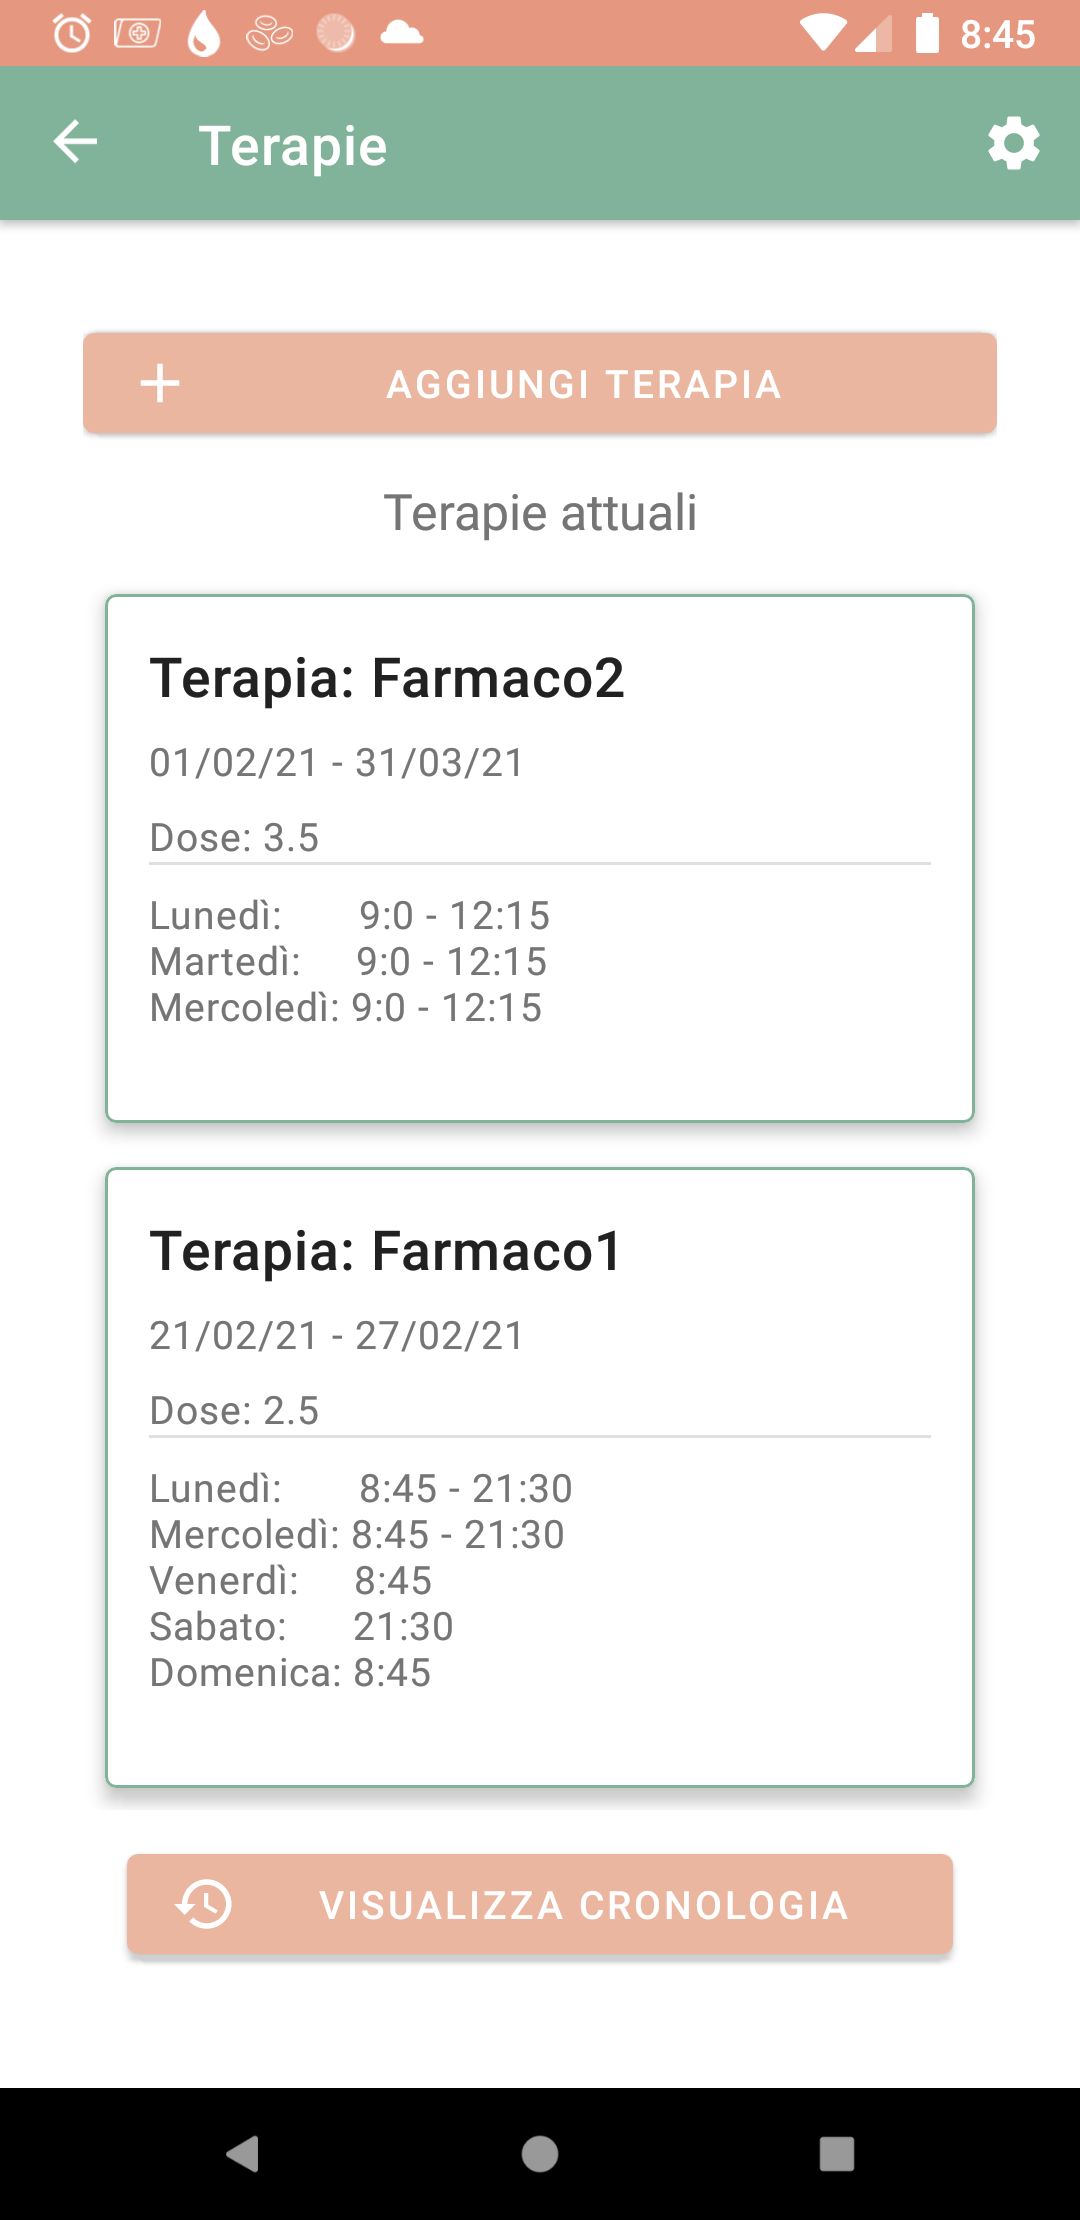
\includegraphics[width=.3\textwidth]{img/Screenshots/Terapie/Fragment.png} \label{terapiaA}} \quad
\subfloat[][\emph{Aggiunta}]
{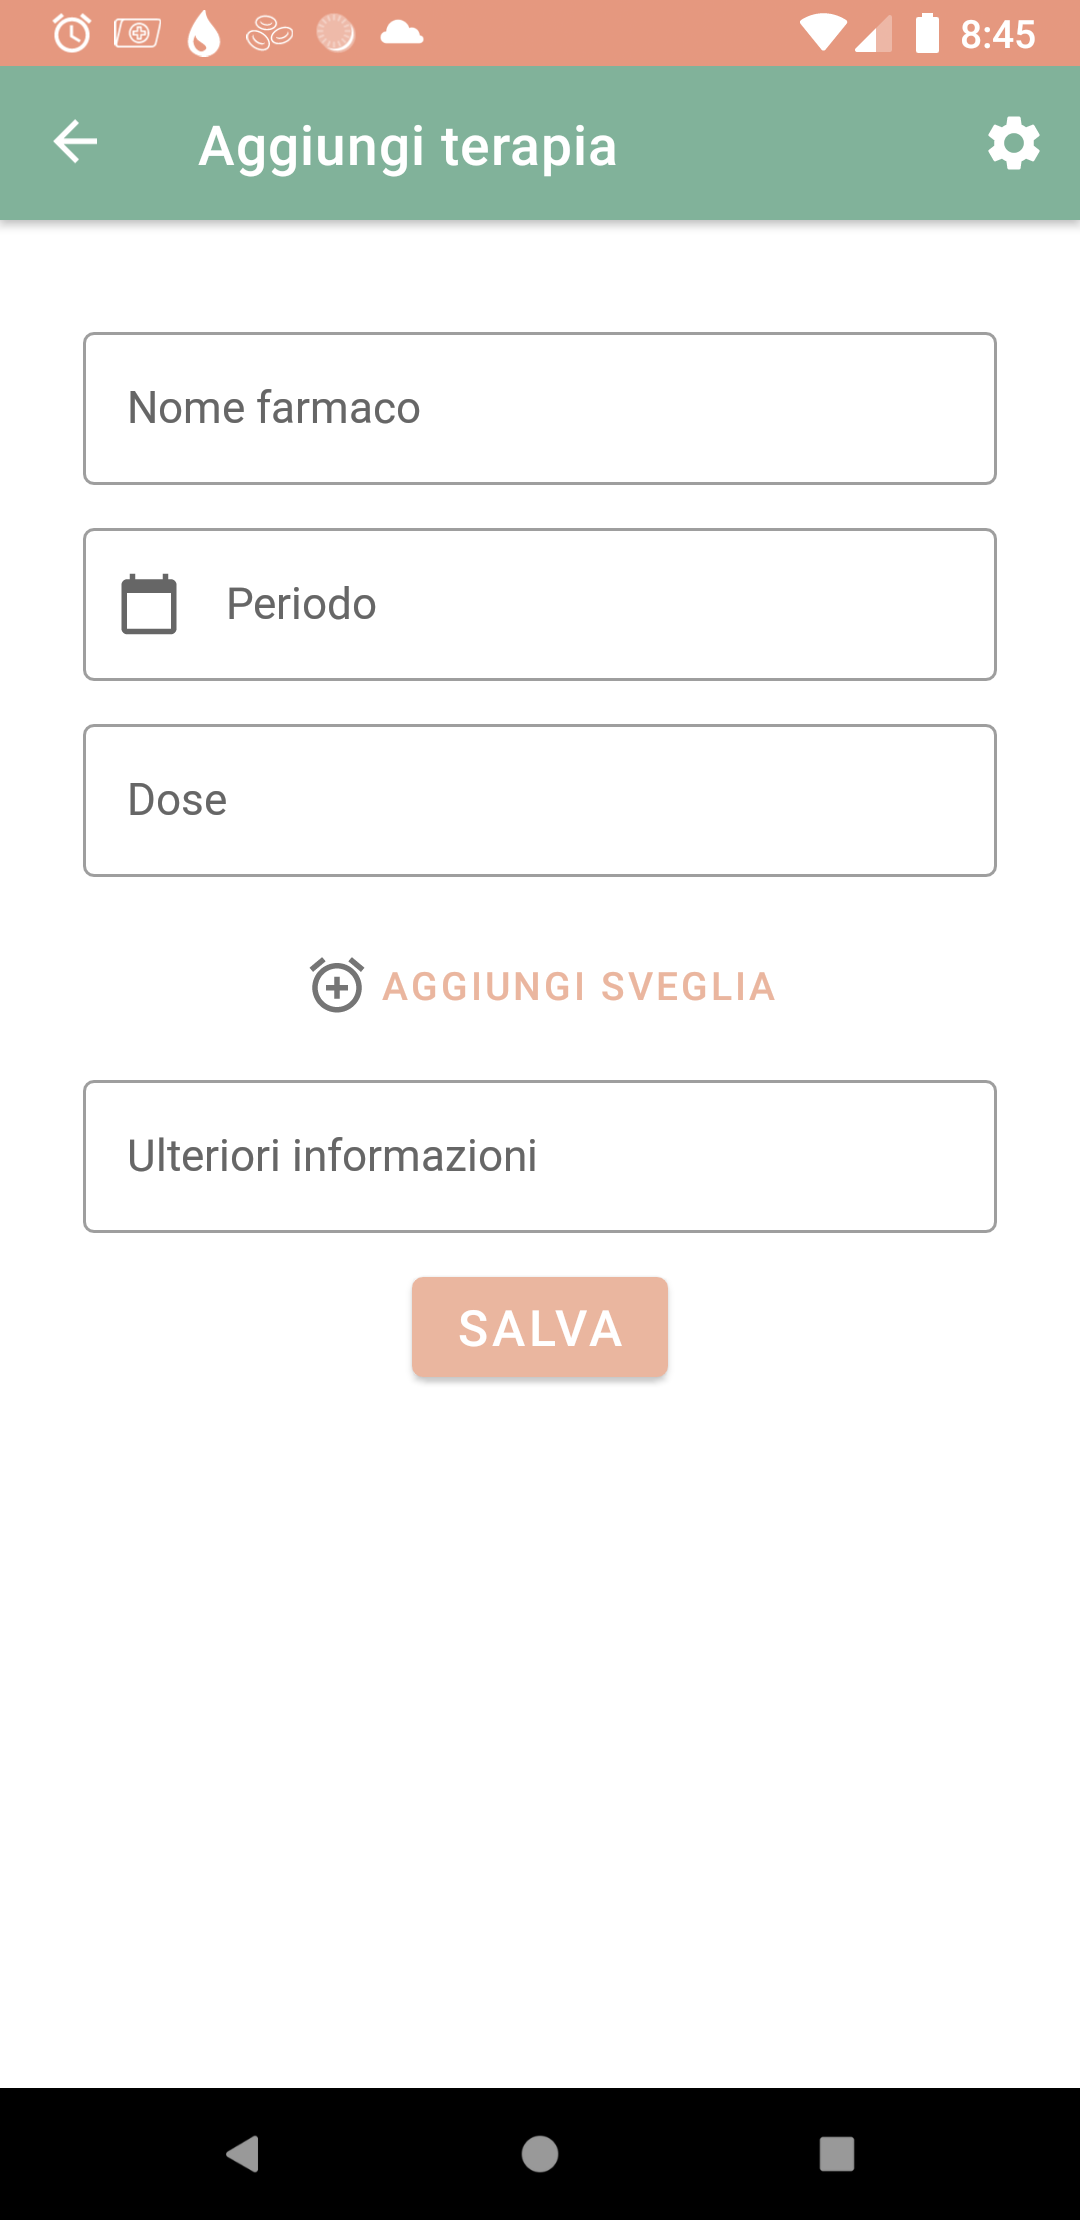
\includegraphics[width=.3\textwidth]{img/Screenshots/Terapie/Aggiungi.png} \label{terapiaB}} \quad
\subfloat[][\emph{Modifica}]
{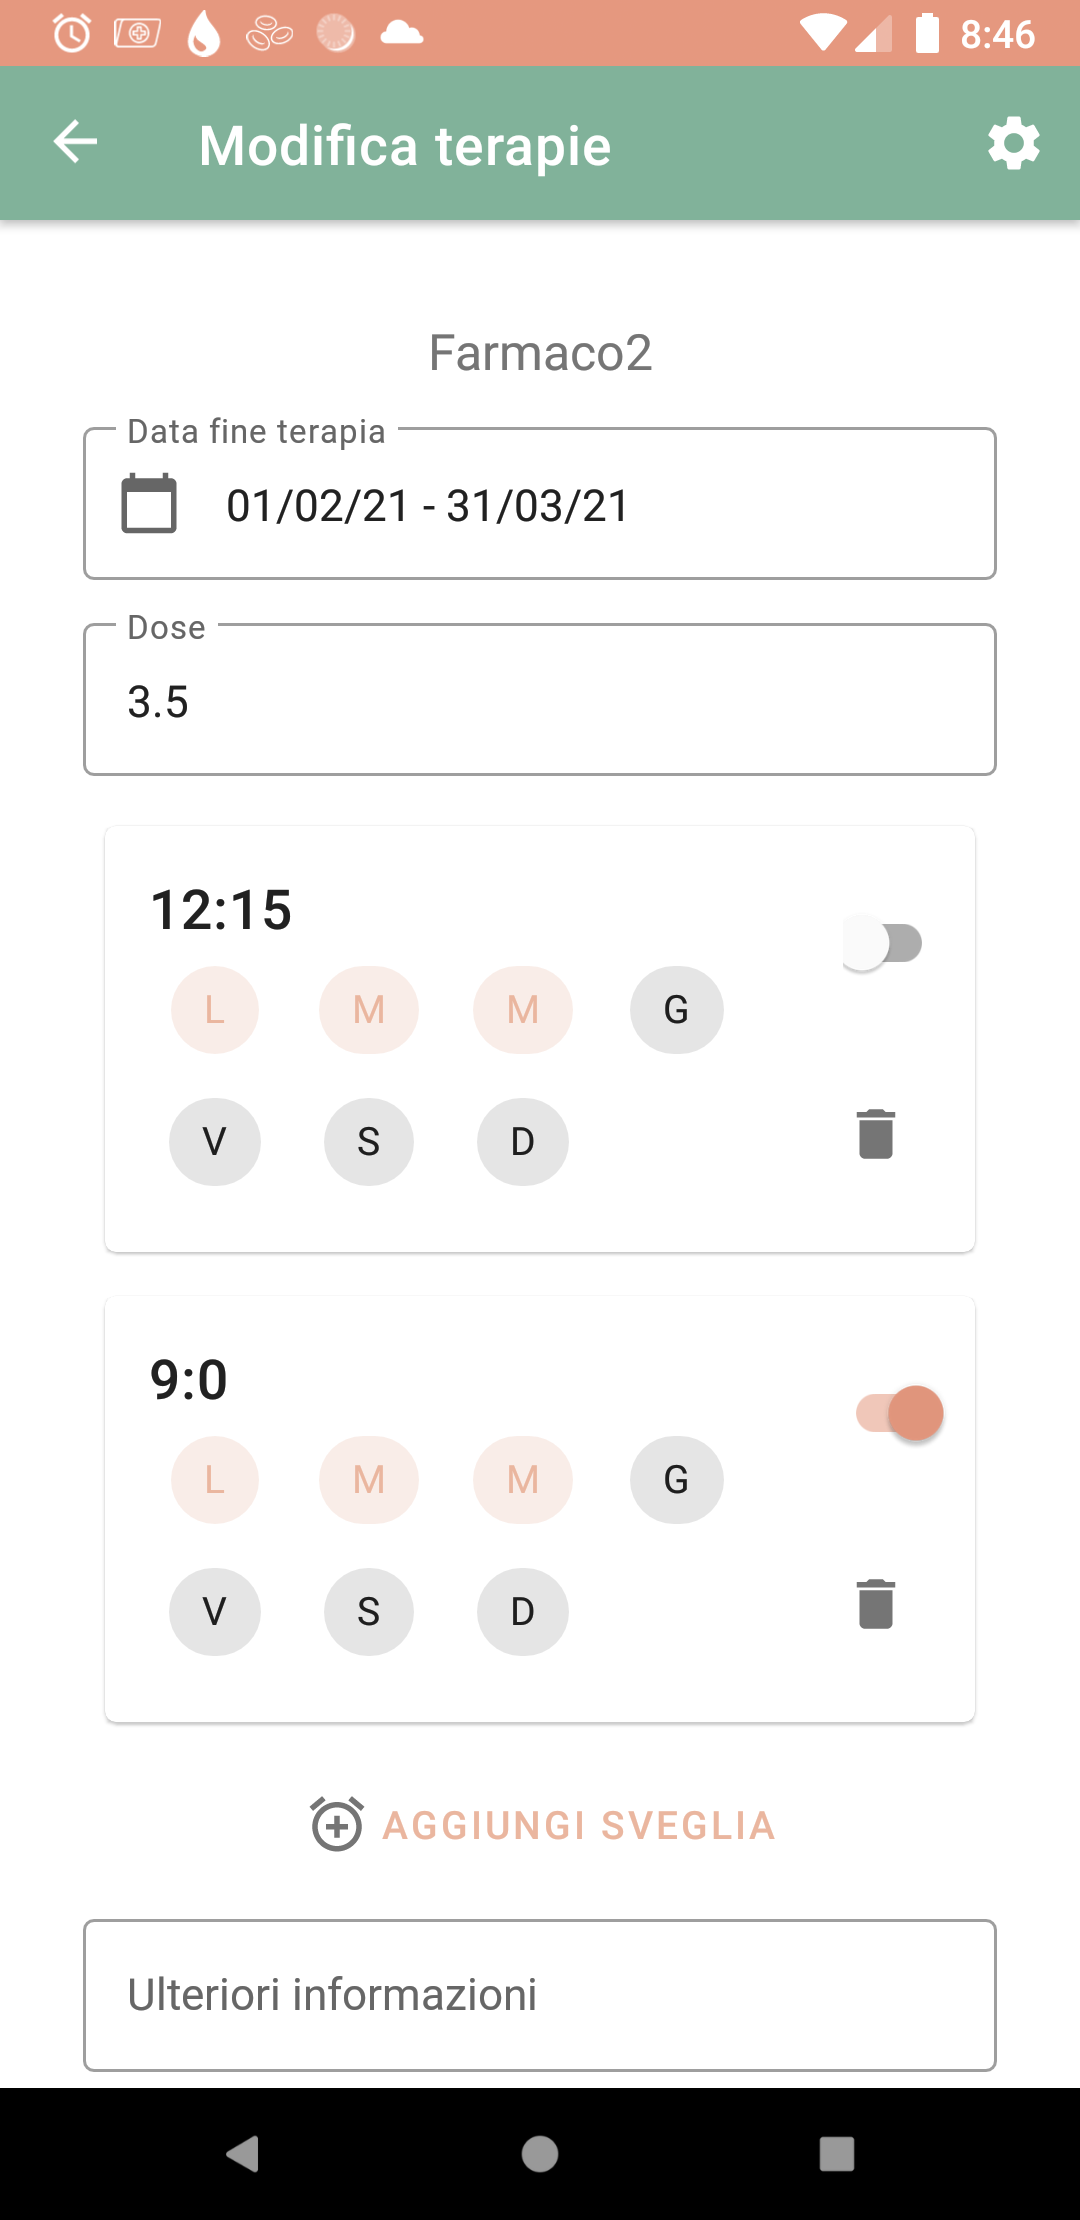
\includegraphics[width=.3\textwidth]{img/Screenshots/Terapie/Modifica.png} \label{terapiaC}} \quad
\caption{Funzionalità riguardanti le terapie}
\label{terapiaD}
\end{figure}


\subsection{Impostazioni e notifiche}
Le impostazioni, sono accessibili dall'icona dell'ingranaggio in alto a destra. Le sue funzionalità \ref{impA} permettono di gestire l'accesso ai dati e la pianificazione delle notifiche. L'utente specifica se intende ricevere o meno avvisi riguardanti: notifiche, esami programmati e non, digiuni e attivazioni anticipate. Nei primi tre casi è consentito specificare l'orario di ricezione della notifica, mentre negli altri due è fissato per le nove di mattina. Una visualizzazione esplicita di come appaiono le notifiche è mostrata in figura \ref{impB}.

Il pulsante in fondo alle impostazioni permette di eseguire il logout e quindi dissociare il proprio account dal dispositivo. Solo in seguito a disconnessione la notifica di TalApp viene rimossa.


\begin{figure}[H]
\centering
\subfloat[][\emph{Impostazioni}]
{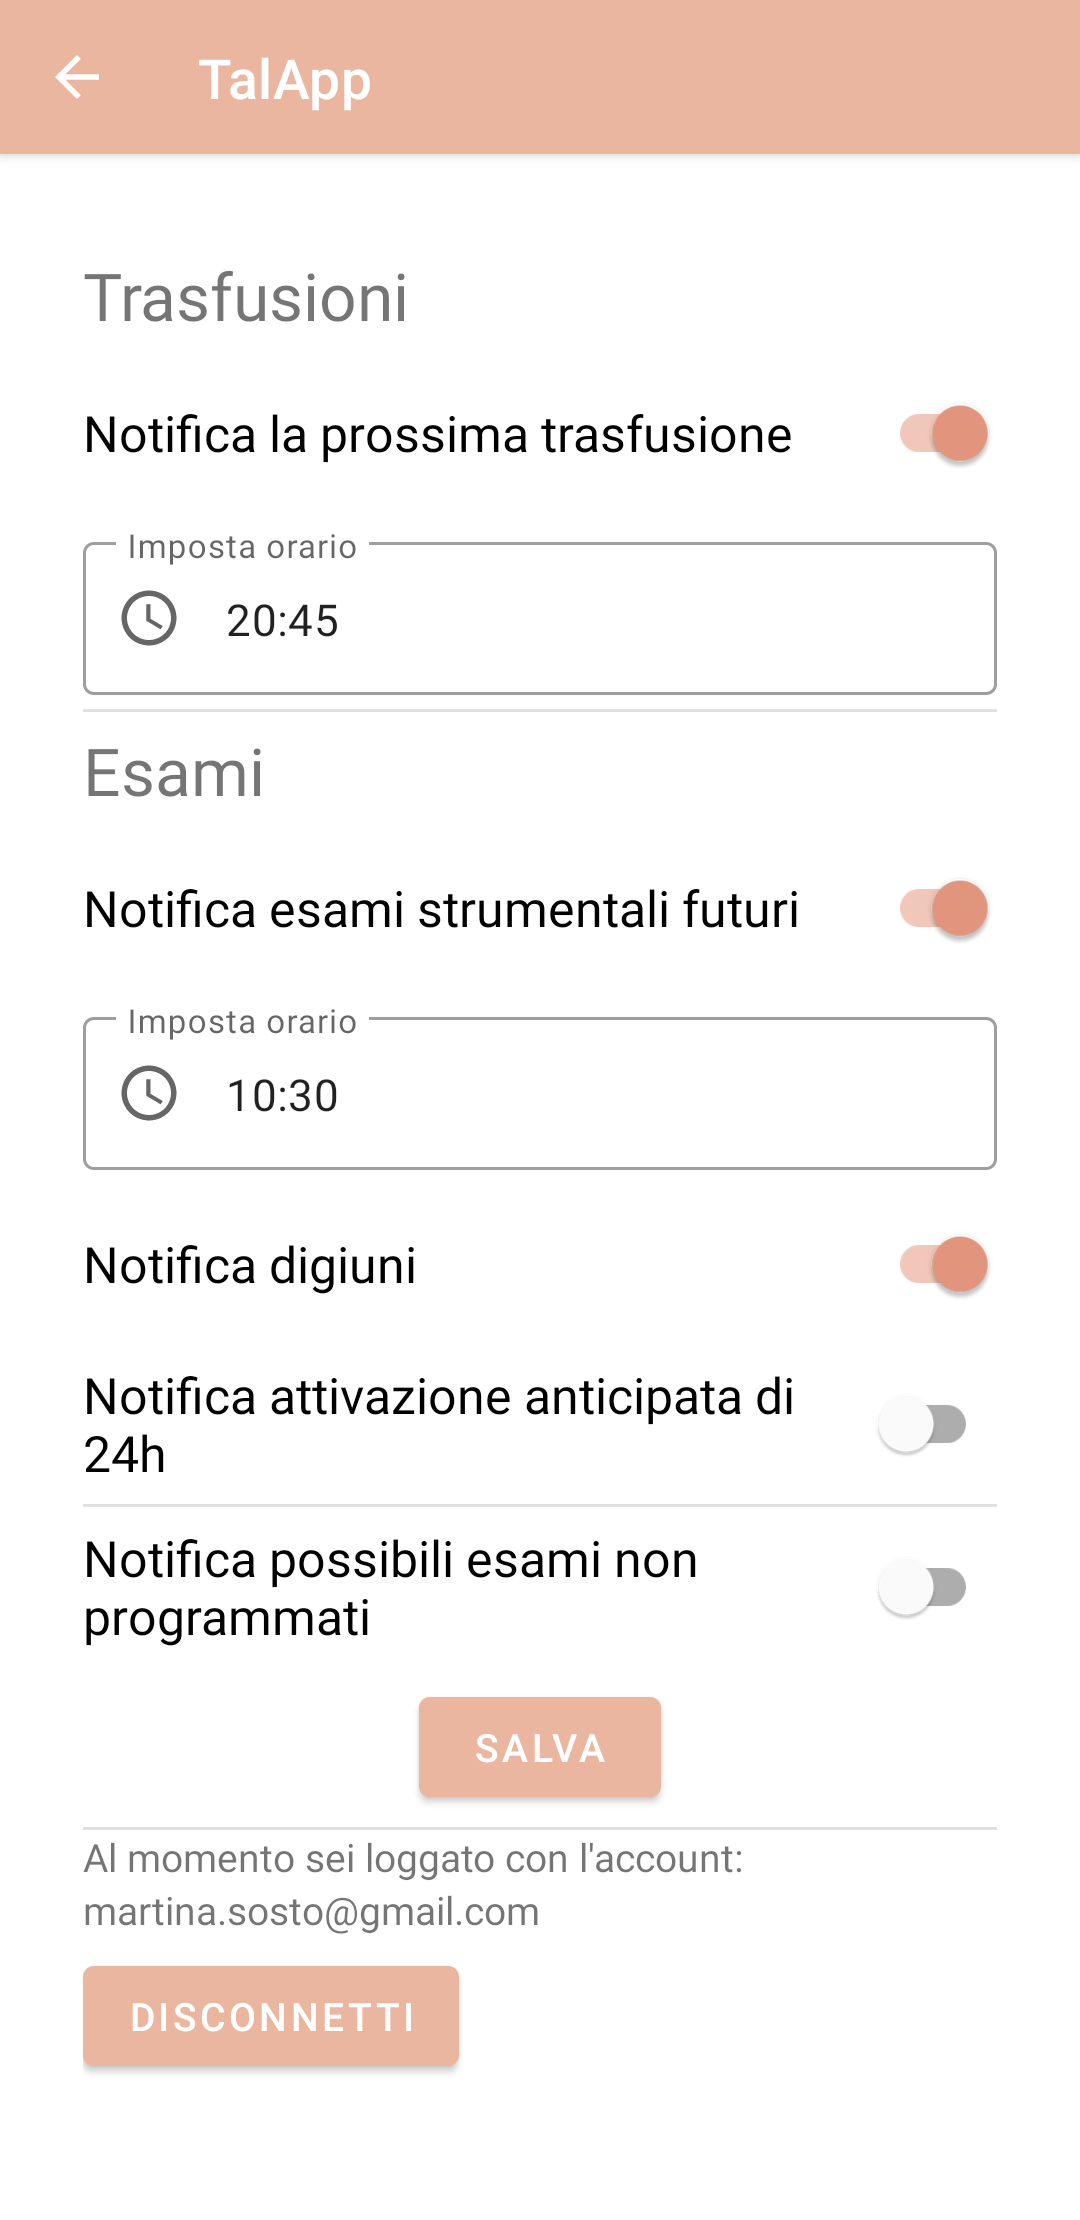
\includegraphics[width=.3\textwidth]{img/Screenshots/Impostazioni/Impostazioni.png} \label{impA}} \quad
\subfloat[][\emph{Notifiche}]
{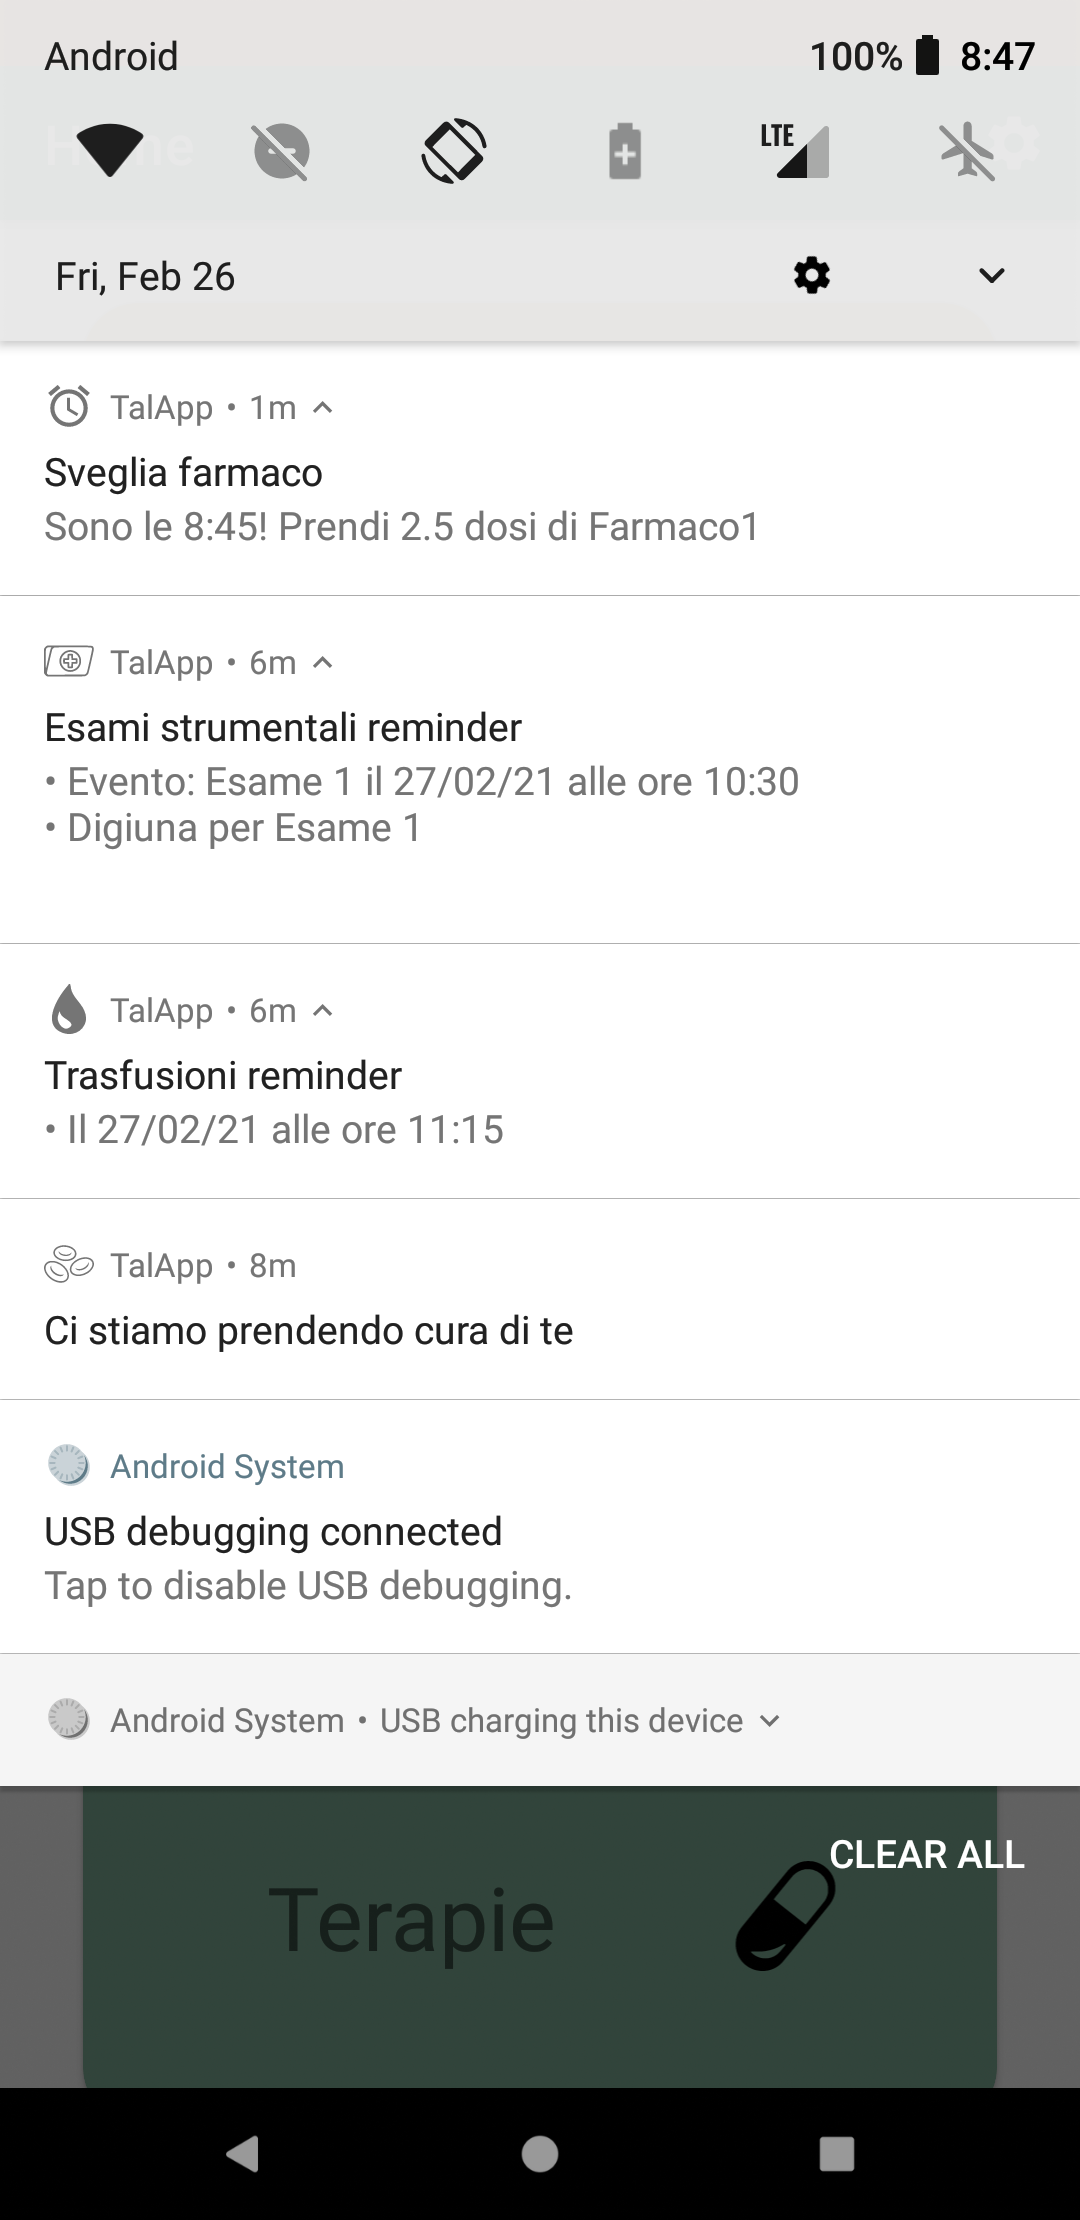
\includegraphics[width=.3\textwidth]{img/Screenshots/Notifiche/Notifiche.png} \label{impB}} \quad
\caption{Funzionalità di notifica e gestione}
\label{impC}
\end{figure}


\chapter{Specifiche tecniche}
In questo capitolo si affronta la parte tecnica: vi è descritto il funzionamento del database, peculiarità del codice, scelte implementative, software e librerie utilizzate e ore di sviluppo dedicate al progetto.

\section{Struttura del database}
Cloud Firestore è stato usato per gestire il database NoSQL  per l'archiviazione e sincronizzazione dei dati. La sua peculiarità è la cache ``illimitata'', le dimensioni reali sono di 100MB ma le informazioni meno recenti vengono costantemente rimpiazzate da nuovi dati utili.
La struttura del database utilizzato è raffigurato nel diagramma ER in figura \ref{ER}. Le entità utilizzate sono in realtà cinque, per la gestione delle analisi viene utilizzata una struttura \verb#Map#. 

\begin{figure}
\begin{center}
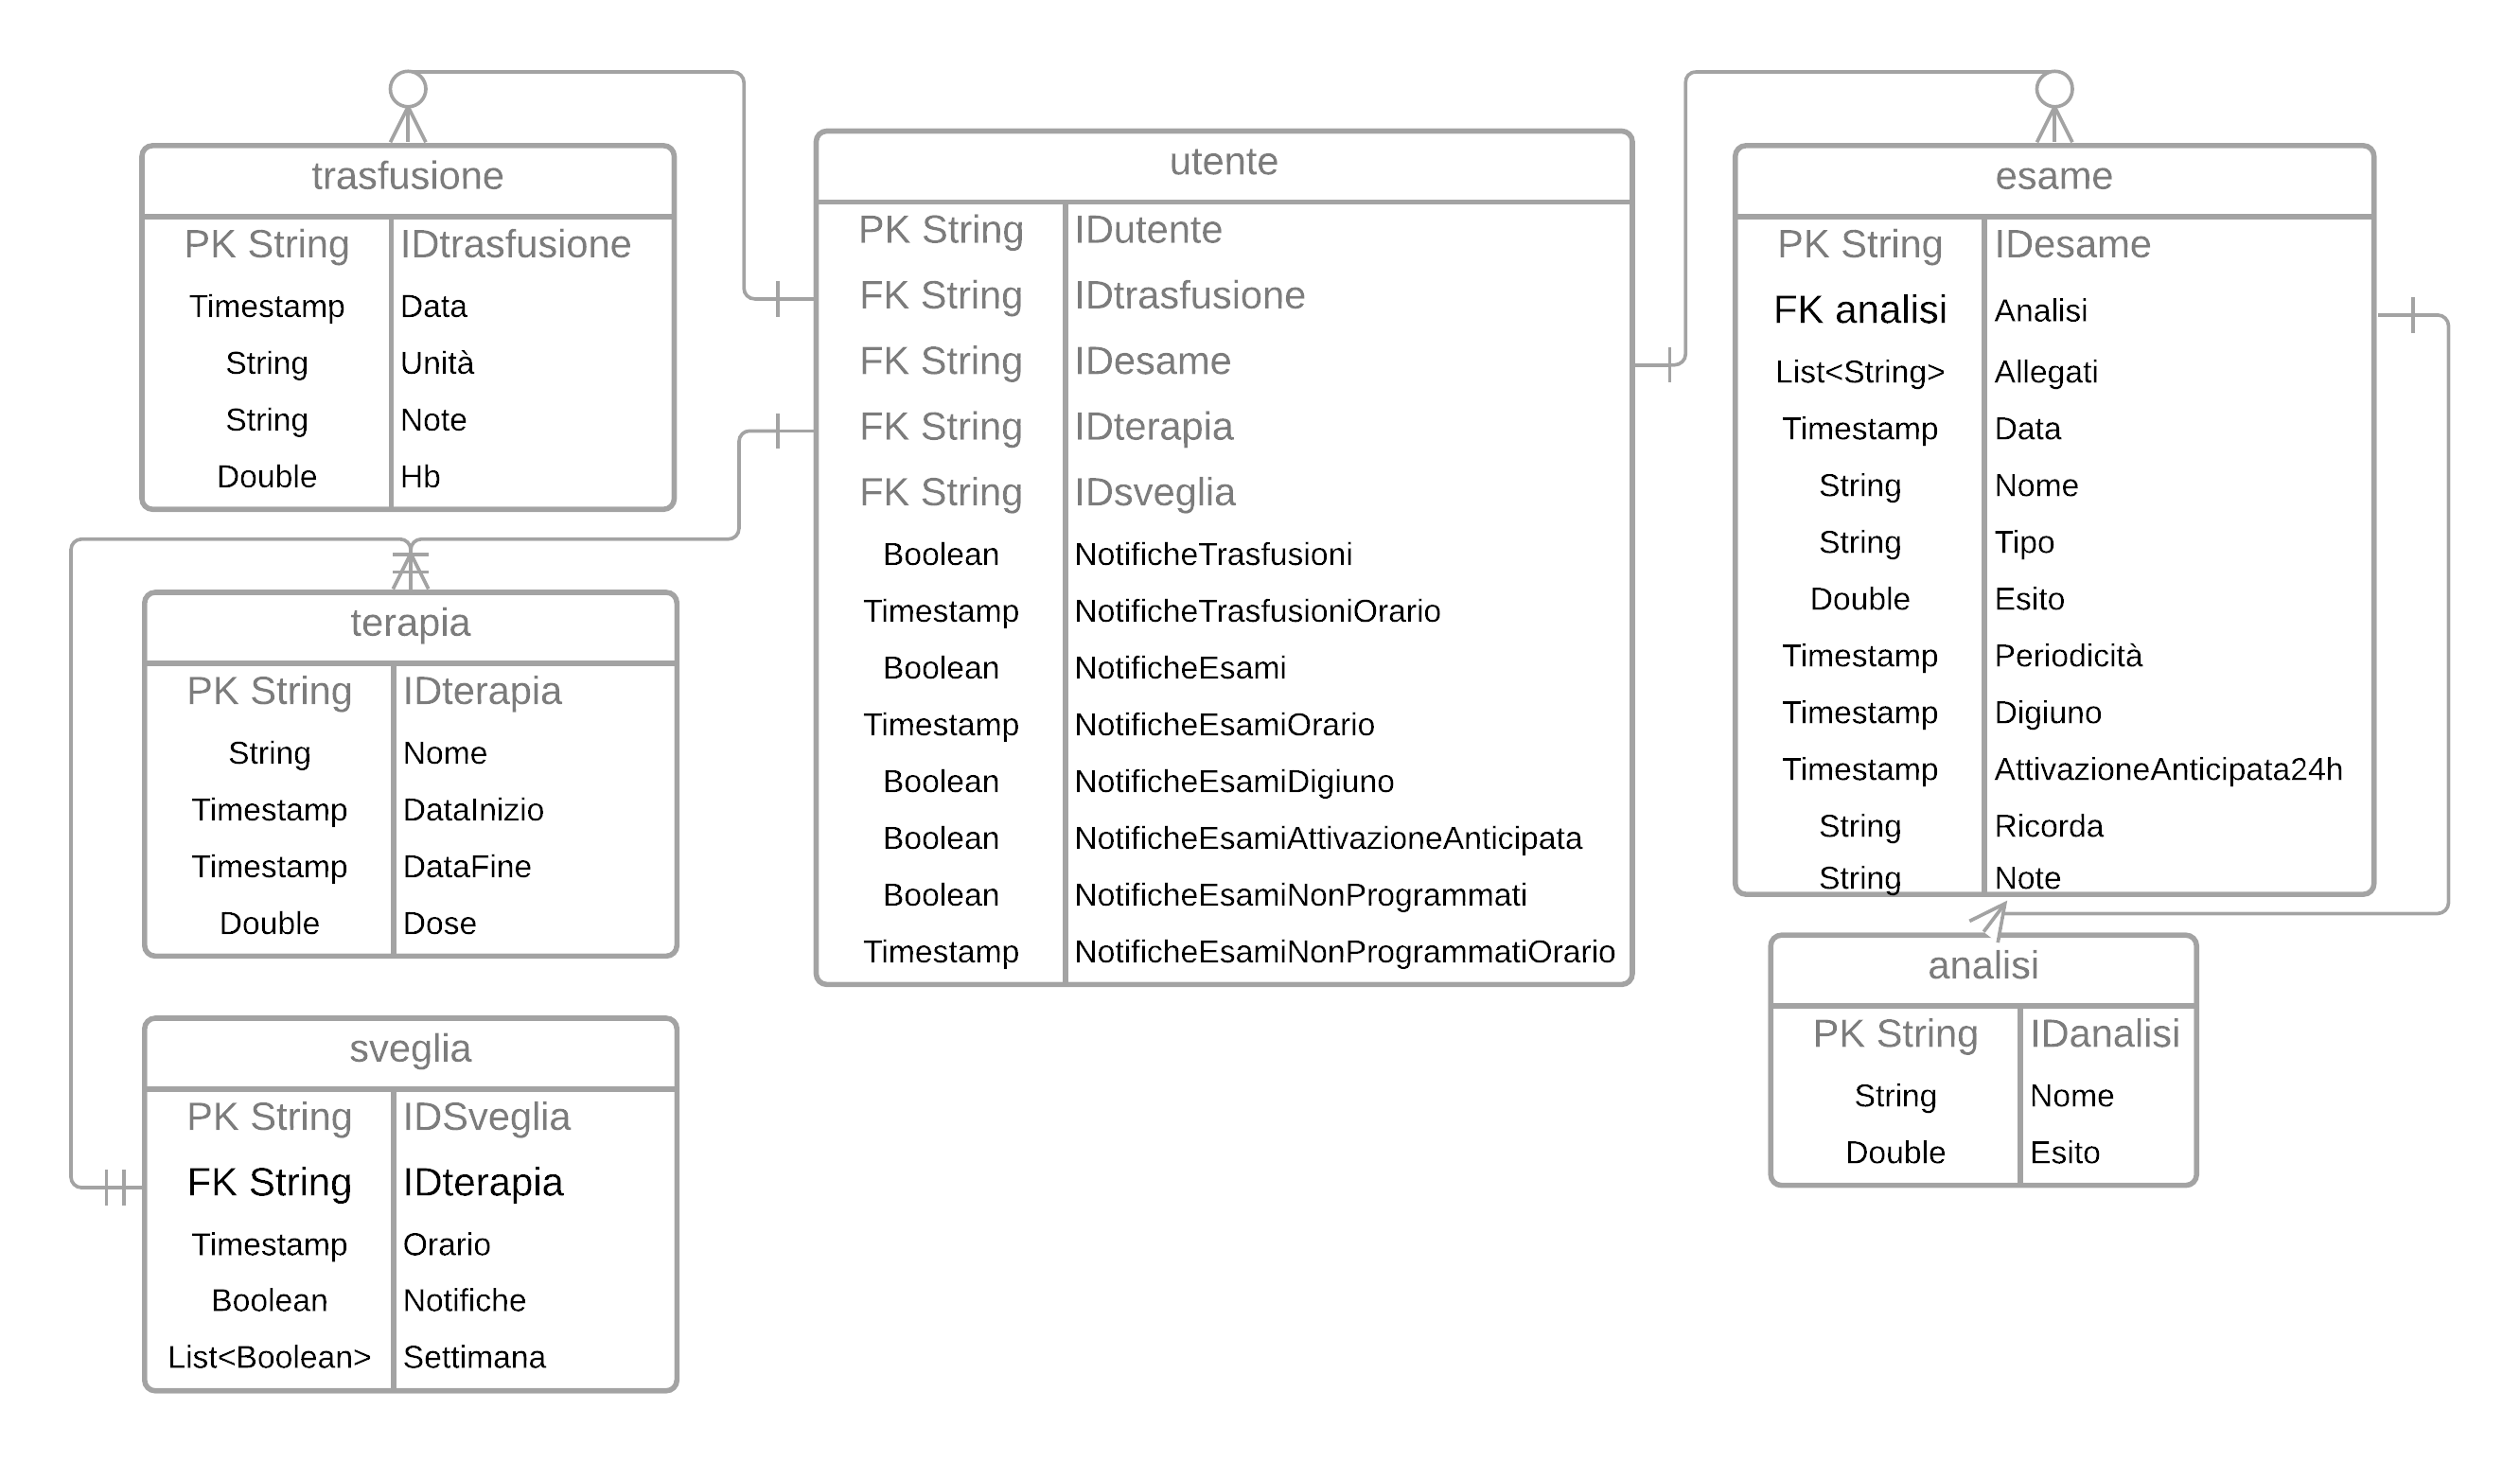
\includegraphics[width=1\textwidth, keepaspectratio]{img/Diagrammi/Diagramma ER.png}
\caption{Diagramma ER} \label{ER}
\end{center}
\end{figure}

L'entità Utente funge da raccolta di informazioni esterne, gli unici dati a sé stanti sono le impostazioni delle notifiche. I campi \verb#Boolean# indicano le preferenze dell'utente nel ricevere o meno notifiche e quelli di tipo \verb#Timestamp# memorizzano gli orari alla quale i suddetti allarmi devono scattare. Tutti i campi possono essere nulli al di fuori della \verb#Primary Key# e dei \verb#Boolean#.

L'entità Esame utilizza i suoi attributi in base alla tipologia d'esame: se di laboratorio allora il campo Analisi contiene almeno un elemento e l'Esito è \verb#null#. Viceversa se l'esame è di tipo strumentale, non contiene una lista di analisi ma l'assegnazione dell'unico esito possibile, situato in Esito. Il valore Periodicità contiene dal primo inserimento il giorno in cui l'esame dovrà ripetersi, il che permette di gestire in modo efficiente le notifiche degli esami non programmati. I campi Digiuno e AttivzioneAnticipata24h sono diversi da \verb#null# solo se contengono la data e l'ora nella quale il paziente deve iniziare il digiuno o essere avvisato in anticipo.

L'entità Trasfusione contiene obbligatoriamente la data e l'unità che devono essere svolte, il campo \verb#Double# Hb è diverso da \verb#null# solo quando viene assegnato.

La tabella Sveglia contiene la una \verb#Foreign Key# (chiave esterna) riferita alla terapia per la quale deve notificare l'utente. Inoltre contiene una lista di \verb#Boolean#, uno per ogni giorno della settimana (\verb#true# se deve notificare l'utente in quel giorno, altrimenti \verb#false#) e un \verb#Boolean# per l'attivazione della sveglia stessa, il che determina se deve suonare o meno.

La Terapia non ha attributi che possono essere \verb#null# e non contiene \verb#Foreign Key# per via del suo collegamento con le sveglie specificato precedentemente.

\section{Frammenti di codice e workflow}
In questa sezione viene trattato un funzionamento peculiare di TalApp, la gestione delle notifiche. Per la visualizzazione di una singola notifica vengono interrogate sei componenti fondamentali:

\begin{enumerate}
    \item Boot Receiver (di tipo BroadcastReceiver): viene risvegliato ogni qualvolta il dispositivo si accende.
    \item Foreground Service (di tipo Service): è una componente che rimane attiva dall'accesso del paziente fino alla disconnessione da TalApp. Il ruolo fondamentale è istanziare il Notification Receiver e fare in modo che non venga mai deallocato, il che permette la corretta ricezione degli allarmi.
    \item Notification Alarm (di tipo Service): tiene traccia dell'orario e della tipologia di ogni allarme che deve scattare.
    \item Job Service (di tipo JobIntentService): interagisce con il Database, controlla i dati e crea la visualizzazione delle notifiche su un thread separato.
    \item Database: contiente i dati dei pazienti.
    \item Notification Receiver (di tipo BroadcastReceiver): viene attivato dall'Notification Alarm, controlla di che tipo è la notifica e inoltra la gestione al Job Service.
\end{enumerate}

Nello schema \ref{notifiche} viene descritta l'interazione tra componenti:

\begin{figure}[H]
\begin{center}
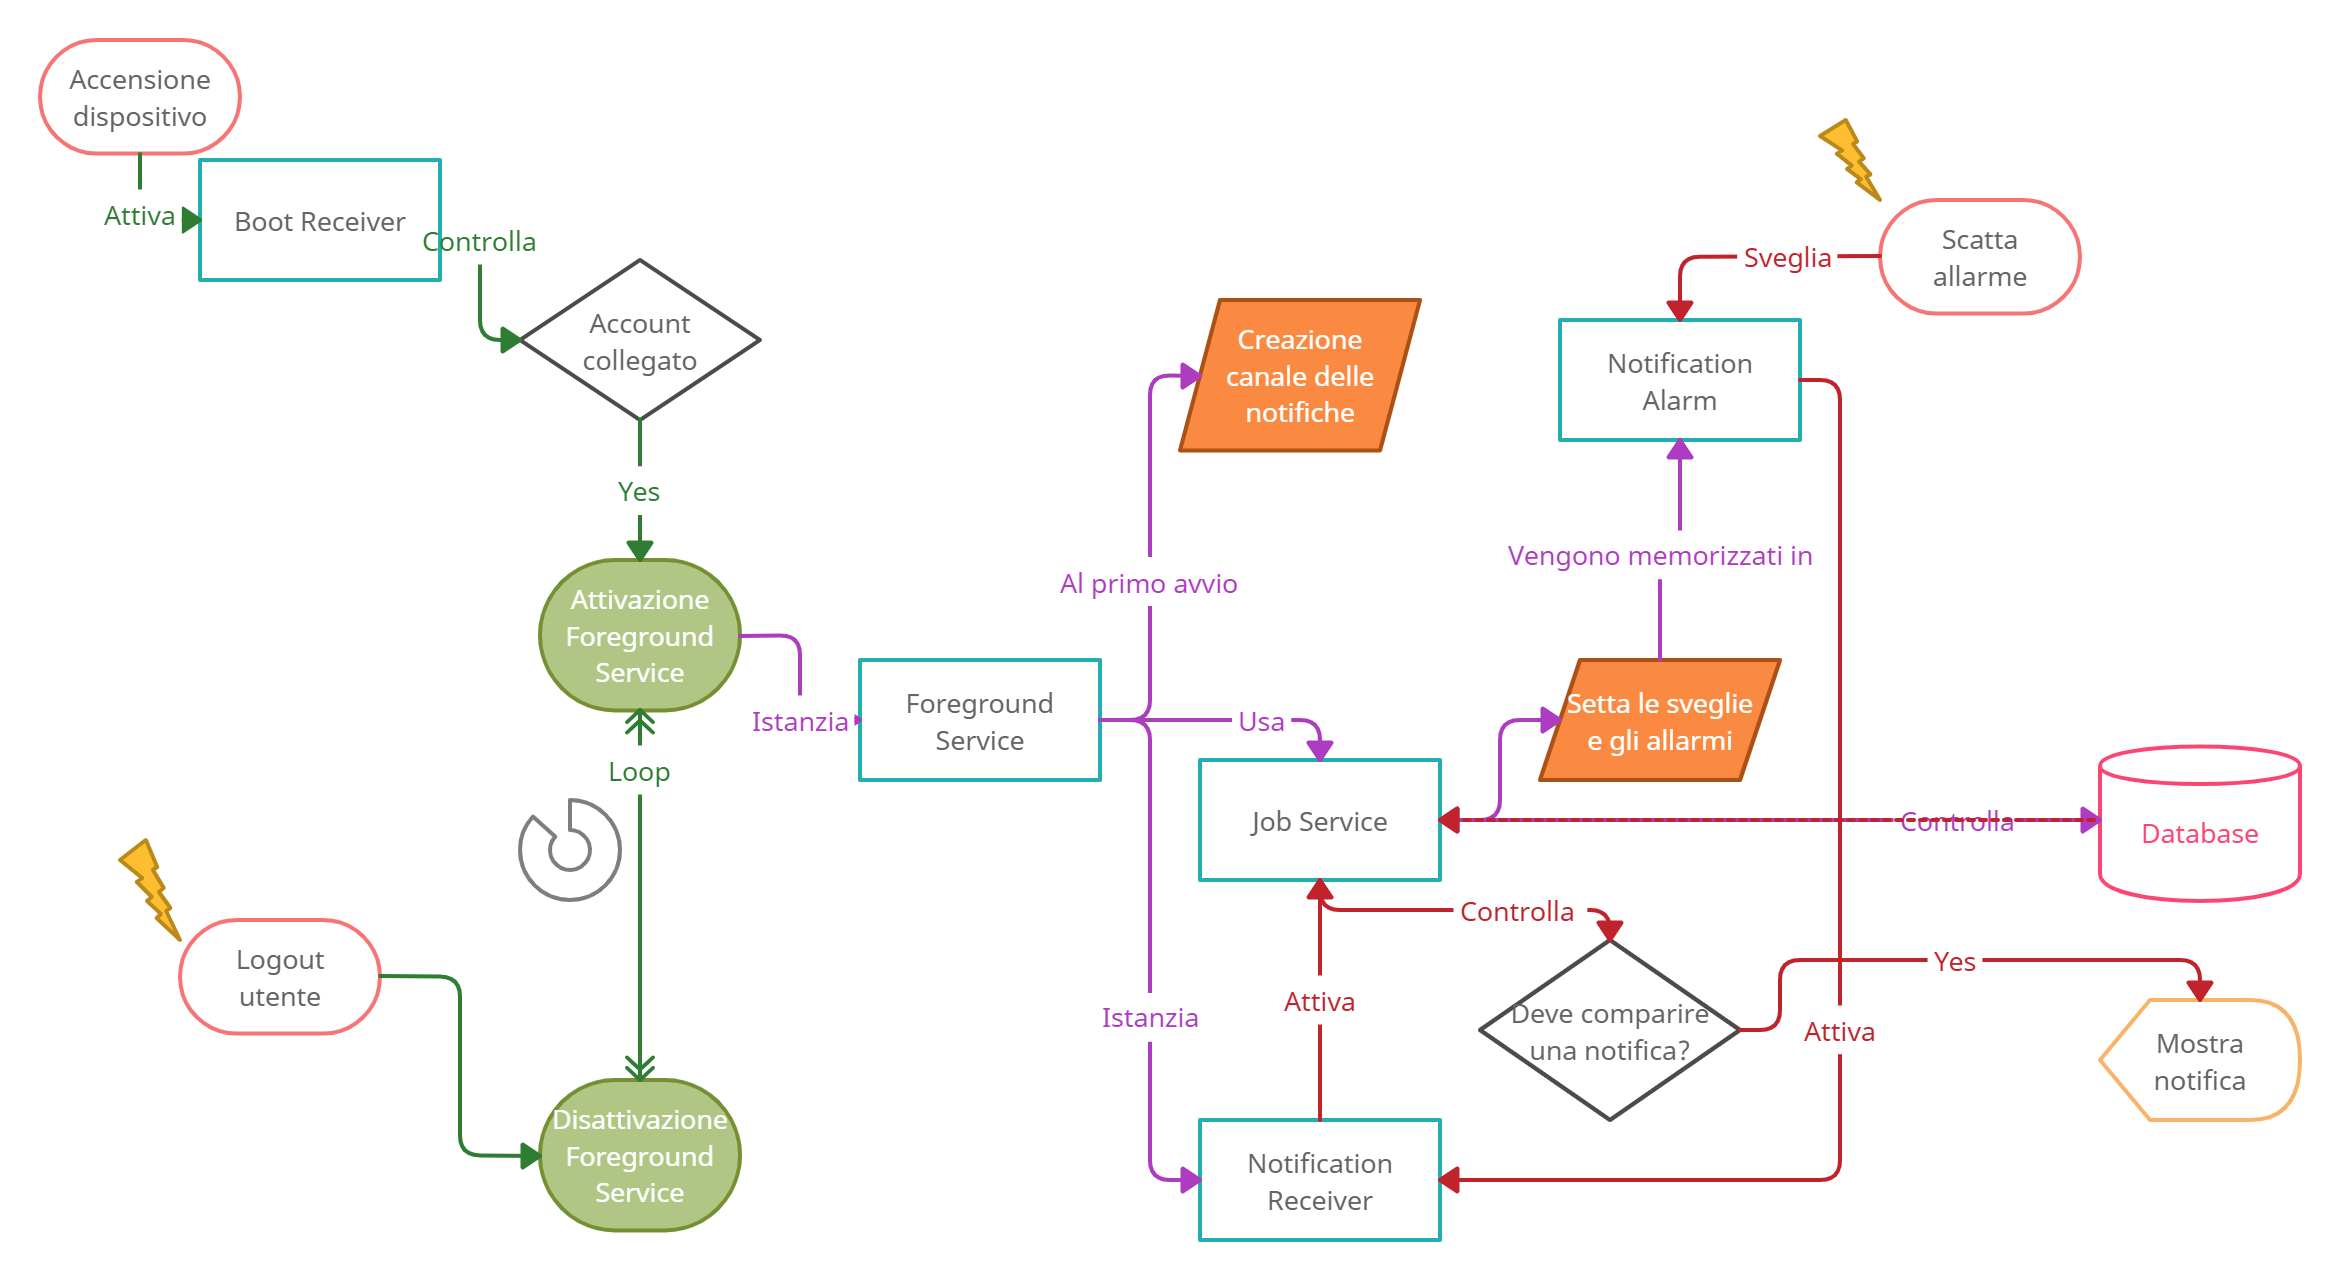
\includegraphics[width=1.2\textwidth, keepaspectratio]{img/Diagrammi/Gestione delle notifiche.png}
\caption{Flusso di gestione delle notifiche} \label{notifiche}
\end{center}
\end{figure}

\begin{itemize}
    \item Flusso verde (solo in fase di inizializzazione): all'accensione del dispositivo il Boot Receiver controlla se il paziente ha effettuato il login, in questo caso attiva il Foreground Service che sarà operante fino alla disconnessione.
    \item Flusso viola (solo in fase di inizializzazione): quando il Foregorund service viene istanziato, crea il canale delle notifiche. Tramite il Job Service, il Notification Alarm e il Database, vengono aggiornate le sveglie settate dal paziente precedentemente.
    \item Flusso rosso: quando scatta un allarme il Notification Alarm viene attivato, di conseguenza diventa operativo il Notification Receiver che tramite il Database e il Job Service permette di far ``disegnare'' la notifica da quest'ultimo.
\end{itemize}

Susseguono frammenti di codice Java che esplicitano le funzionalità descritte precedentemente.

Classe Boot Receiver:
\begin{lstlisting}[language = Java , frame = trBL , firstnumber = last , escapeinside={(*@}{@*)}] 
public class BootReceiver extends BroadcastReceiver {
    @Override
    public void onReceive(Context aContext, Intent aIntent) {
        Intent serviceIntent = new Intent(aContext, ForegroundService.class);
        ContextCompat.startForegroundService(aContext, serviceIntent); //Attiva il Foreground Service
    }
}
\end{lstlisting}

Classe Notification Receiver:
\begin{lstlisting}[language = Java , frame = trBL , firstnumber = last , escapeinside={(*@}{@*)}]
public class NotificationReceiver extends BroadcastReceiver {
    @Override
    public void onReceive(Context context, Intent intent) {
        Intent serviceIntent = new Intent(context, JobService.class);
        if(intent.getAction().equals(ACTION_CLOCK)){ //Raccoglie le informazioni dell'allarme attivato
            serviceIntent.putExtra("SVEGLIA", intent.getStringExtra("SVEGLIA"));
        }
        serviceIntent.setAction(intent.getAction());
        JobService.enqueueWork(context, serviceIntent); //Inoltra il lavoro al Job Service
    }
}
\end{lstlisting}

Funzione che imposta gli allarmi nel Notification Alarm:
\begin{lstlisting}[language = Java , frame = trBL , firstnumber = last , escapeinside={(*@}{@*)}]
public static void setAlarm(Date Orario, int IDAllarme, String CampoBooleano){
        Date date = Calendar.getInstance().getTime();
        Orario.setYear(date.getYear());
        Orario.setMonth(date.getMonth());
        Orario.setDate(date.getDate());
        Calendar cal = Calendar.getInstance();
        cal.setTime(Orario);
        if(Orario.compareTo(date) <= 0 ) cal.add(Calendar.DATE, 1); //Se l'orario alla quale deve scattare la notifica e' gia' passato allora la farà suonare nella giornata successiva
        Intent intent = new Intent(context, NotificationReceiver.class);
        intent.setAction(CampoBooleano);
        PendingIntent pendingIntent = PendingIntent.getBroadcast(context, IDAllarme, intent, PendingIntent.FLAG_UPDATE_CURRENT);
        alarmManager.setRepeating(android.app.AlarmManager.RTC_WAKEUP, cal.getTimeInMillis(), AlarmManager.INTERVAL_DAY, pendingIntent); //Imposta l'orario e le ripetizioni da svolgere inerentin all'allarme
    }
\end{lstlisting}

Funzione del Job Intent Service che richiama diverse funzioni in base alla tipologia di lavoro da svolgere:
\begin{lstlisting}[language = Java , frame = trBL , firstnumber = last , escapeinside={(*@}{@*)}]
@Override
    protected void onHandleWork(@NonNull Intent intent) {
        switch (intent.getAction()){
            case ACTION_SET_NOTIFICATION_ALARMS:
                setNotificationAlarms();
                break;
            case ACTION_SET_CLOCK_ALARMS:
                setClockAlarms();
                break;
            case IMPOSTAZIONI_TRASFUSIONI:
                getNextTrasfusione();
                break;
            case IMPOSTAZIONI_ESAMI:
                getNextEsame();
                break;
            case IMPOSTAZIONI_ESAMI_PERIODICI:
                getNextEsamePeriodico();
                break;
            case ACTION_CLOCK:
                getFarmaco(intent);
                break;
        }
    }
\end{lstlisting}

Funzioni che controllano quali terapie devono essere notificate e creano la visualizzazione effettiva del componente grafico visualizzato:
\begin{lstlisting}[language = Java , frame = trBL , firstnumber = last , escapeinside={(*@}{@*)}]
    private void getFarmaco(Intent intent) {
        String idSveglia = intent.getStringExtra("SVEGLIA");

        
        sveglieRef.document(idSveglia).get().addOnCompleteListener(task -> { //Vengono reperite le informazioni sulla sveglia scattata
            Map<String, Object> sveglia = task.getResult().getData();
            if(((Boolean)sveglia.get(KEY_NOTIFICHE) && Util.getNumeroGiornoDaSettimana((List<Boolean>) sveglia.get(KEY_SETTIMANA)))){
                //In questo caso le notifiche sono accese e la sveglia deve suonare
                terapieRef.document((String) sveglia.get(KEY_FARMACO)).get().addOnCompleteListener(task1 -> {
                    Map<String, Object> terapia = task1.getResult().getData();
                    Date dataFine = Util.TimestampToDate((Timestamp) terapia.get(KEY_DATA_FINE));
                    //Viene controllata la data di fine terapia per comprendere se il giorno di oggi è compreso tra questi
                    if(dataFine.compareTo(Util.getPrimoMinuto(Calendar.getInstance()).getTime()) >= 0){ //In questo caso viene sollevata una notifica
                    
                        NotificationManagerCompat notificationManagerCompat = NotificationManagerCompat.from(getApplicationContext());
                        notificationManagerCompat.notify(ID_SVEGLIE, getSveglieNotification("Sono le " + Util.TimestampToOrario((Timestamp) sveglia.get(KEY_ORARIO)) + "! Prendi " + terapia.get(KEY_DOSE) + " dosi di " + terapia.get(KEY_NOME), getApplicationContext()).build());
                    }
                });
            }
        });
    }

    //Crea la notifica
    private static NotificationCompat.Builder getSveglieNotification(String messaggio, Context mContext) {
        NavDeepLinkBuilder navDeepLinkBuilder = new NavDeepLinkBuilder(mContext);
        PendingIntent pendingIntent = navDeepLinkBuilder.setComponentName(HomeActivity.class)
                .setGraph(R.navigation.nav_graph_home)
                .setDestination(R.id.terapieFragment)
                .createPendingIntent();

        NotificationCompat.Builder builder = new NotificationCompat.Builder(mContext, SVEGLIE_CHANNEL);
        builder.setSmallIcon(R.drawable.ic_baseline_access_alarm_24)
                .setContentTitle("Sveglia farmaco")
                .setStyle(new NotificationCompat.BigTextStyle()
                        .bigText(messaggio))
                .setPriority(NotificationCompat.PRIORITY_DEFAULT)
                .setContentIntent(pendingIntent)
                .setAutoCancel(true);
        return builder;
    }
\end{lstlisting}

\section{Scelte implementative}
Vengono elencate alcune scelte implementative e accorgimenti riscontrati durante lo sviluppo:

\begin{enumerate}
    \item Il design grafico semplice e con poche componenti è stato disegnato in modo tale da rendere l'utente meno disinvolto nell'utilizzo di tecnologia proprio agio in fase di utilizzo. I colori rimangono gli stessi nelle varie sezioni per facilitare l'orientamento nel grafo delle schermate.
    \item Sono state implementate funzioni di gestione di soli eventi comuni come trasfusioni, esami e terapie perché sono le categorie che più necessitano di accorgimenti da parte del paziente talassemico.
    \item Si \`e ritenuto necessario includere un portale di login per garantire riservatezza dei dati personali del paziente. \`E stato integrato l'accesso tramite Google comodità d'uso.
    \item Si sono distinte le due tipologie di esame per rendere più facile all'utente l'inserimento degli esisti.
    \item Per ricercare i dati nel database quando si solleva un allarme di notifica è stato utilizzato un JobInentService che permette di lavorare su un thread separato.
    \item Essendo il database utente sempre aggiornato - grazie alla cache - il controllo della comparsa di notifiche è stato svolto allo scattare dell'allarme stesso. In altri termini, l'Alarm Manager ha Intent pendenti prefissati all'orario di ricezione scelto dall'utente, solo in quel momento, viene controllato il database e la notifica appare solo se ci sono degli eventi da notificare.
    \item L'istanza del Notification Receiver si trova nel Foreground Service per assicurarsi che fosse sempre pronta a ricevere anche quando la Main Activity è stata distrutta.
\end{enumerate}

\section{Report e monte ore}
Per la costruzione dell'intero progetto sono state investite oltre 200 ore, di cui 180 di programmazione e sviluppo e 67 release ufficiali. Raccolti in tabella \ref{MonteOre}  ci sono report inerenti a ogni processo che ha reso TalApp il prodotto che è attualmente.

% Please add the following required packages to your document preamble:
% \usepackage{longtable}
% Note: It may be necessary to compile the document several times to get a multi-page table to line up properly
\begin{longtable}{|l|l|l|l|}
\hline
\textbf{Giorno} &
  \textbf{Ore} &
  \textbf{Attività} &
  \textbf{Versione} \\ \hline
\endhead
%
15/12/2020 &
  4 &
  Disegno mockup e stesura obiettivi e requisiti &
   \\ \hline
21/12/2020 &
  2 &
  Disegno layout &
  \begin{tabular}[c]{@{}l@{}}TalApp\\ TalApp1\end{tabular} \\ \hline
22/12/2020 &
  8 &
  \begin{tabular}[c]{@{}l@{}}Ricerca sulla piattaforma Firebase per capire come\\  gestire le autenticazioni\\ Progettare layout\end{tabular} &
  \begin{tabular}[c]{@{}l@{}}TalApp2\\ TalApp3\end{tabular} \\ \hline
23/12/2020 &
  8 &
  \begin{tabular}[c]{@{}l@{}}Creazione login e registrazione tramite Firebase\\  Authentication\end{tabular} &
  \begin{tabular}[c]{@{}l@{}}TalApp4\\ TalApp5\end{tabular} \\ \hline
24/12/2020 &
  6 &
  Creazione e modifica di layout &
  \begin{tabular}[c]{@{}l@{}}TalApp6\\ TalApp7\end{tabular} \\ \hline
25/12/2020 &
  4 &
  \begin{tabular}[c]{@{}l@{}}Creazione layout Implementazione Navigation\\ Schematizzazione struttura app\end{tabular} &
  TalApp8 \\ \hline
26/12/2020 &
  4 &
  \begin{tabular}[c]{@{}l@{}}Ricerca su Cloud Firebase DB\\ Applicazione di navigation sui layout creati\\ Creazione layout\end{tabular} &
  \begin{tabular}[c]{@{}l@{}}TalApp9\\ TalApp10\\ TalApp11\\ TalApp12\end{tabular} \\ \hline
27/12/2020 &
  6 &
  \begin{tabular}[c]{@{}l@{}}Gestione login in assenza di connessione\\ Implementazione funzionalità per l’inserimento\\  dei dati in Colud Firebase DB\end{tabular} &
  \begin{tabular}[c]{@{}l@{}}TalApp13\\ TalApp14\\ TalApp15\end{tabular} \\ \hline
28/12/2020 &
  2 &
  \begin{tabular}[c]{@{}l@{}}Ho inserito il codice che permette l'inserimento\\  di una trasfusione\end{tabular} &
  TalApp16 \\ \hline
29/12/2020 &
  5 &
  \begin{tabular}[c]{@{}l@{}}Implementazione login tramite Google\\ Implementazione inserimento dati trasfusioni\\ Implementazione della visualizzazione dati \\ trasfusioni in calendario\end{tabular} &
  \begin{tabular}[c]{@{}l@{}}TalApp17\\ TalApp18\end{tabular} \\ \hline
30/12/2020 &
  7 &
  \begin{tabular}[c]{@{}l@{}}Reformat colori della app\\ Implementazione inserimento e modifica\\  trasfusioni\end{tabular} &
  \begin{tabular}[c]{@{}l@{}}TalApp19\\ TalApp20\\ TalApp21\end{tabular} \\ \hline
31/12/2020 &
  3 &
  \begin{tabular}[c]{@{}l@{}}Implementazione inserimento, modifica, \\ eliminazione trasfusioni\end{tabular} &
  TalApp22 \\ \hline
01/01/2021 &
  2 &
  Ricerca su Cloud Firebase DB &
  TalApp23 \\ \hline
01/02/2021 &
  5 &
  \begin{tabular}[c]{@{}l@{}}Implementazione inserimento esami\\ Implementazione foreground service e \\ il broadcast receiver\end{tabular} &
  \begin{tabular}[c]{@{}l@{}}TalApp23\\ TalApp24\end{tabular} \\ \hline
01/03/2021 &
  1 &
  \begin{tabular}[c]{@{}l@{}}Implementazione inserimento, modifica, \\ eliminazione esami\end{tabular} &
  TalApp25 \\ \hline
01/09/2021 &
  2 &
  \begin{tabular}[c]{@{}l@{}}Implementazione visualizzazione eventi \\ in calendario\end{tabular} &
  TalApp26 \\ \hline
01/11/2021 &
  1 &
  Implementazione notifiche &
  TalApp27 \\ \hline
01/12/2021 &
  2 &
  \begin{tabular}[c]{@{}l@{}}Riformattazione del codice \\ (schema View Model eliminato)\\ Modifiche visualizzazione layout esami\\ Implementazione impostazioni\end{tabular} &
  TalApp28 \\ \hline
13/1/2021 &
  3 &
  Ottimizzazione visualizzazione eventi in calendario &
  TalApp29 \\ \hline
14/1/2021 &
  3 &
  \begin{tabular}[c]{@{}l@{}}Ricerca su pending intent per l'implementazione\\  delle notifiche\end{tabular} &
  TalApp30 \\ \hline
15/1/2021 &
  3 &
  \begin{tabular}[c]{@{}l@{}}Ottimizzazione visualizzazione eventi giornalieri\\ Ottimizzazione ricezione dati tramite cache\end{tabular} &
  TalApp31 \\ \hline
16/1/2021 &
  5 &
  Ottimizzazione e correzzione bug impostazioni &
  TalApp32 \\ \hline
21/1/2021 &
  3 &
  Correzione bug &
  TalApp35 \\ \hline
24/1/2021 &
  8 &
  \begin{tabular}[c]{@{}l@{}}Implementazione JobIntentService per la \\ gestione delle notifiche\end{tabular} &
  TalApp36 \\ \hline
26/1/2021 &
  4 &
  Implementazione notifiche esami e trasfusioni &
  TalApp37 \\ \hline
27/1/2021 &
  6 &
  \begin{tabular}[c]{@{}l@{}}Completamento implementazione notifiche \\ esami anticpati\\ Ottimizzazione implementazione notifiche esami\\  e trasfusioni\\ Inizio creazione notifiche per terapie\end{tabular} &
  \begin{tabular}[c]{@{}l@{}}TalApp37\\ TalApp38\end{tabular} \\ \hline
29/1/2021 &
  5 &
  \begin{tabular}[c]{@{}l@{}}Implementazione inserimento, modifica \\ ed eliminazione terapie \\ Implementazione visualizzazione terapie\\  in calendario\end{tabular} &
  \begin{tabular}[c]{@{}l@{}}TalApp39\\ TalApp40\\ TalApp41\end{tabular} \\ \hline
30/1/2021 &
  1 &
  Progettazione layout per sveglie &
  TalApp42 \\ \hline
31/1/2021 &
  3 &
  Implementazione sveglie &
  TalApp43 \\ \hline
02/01/2021 &
  5 &
  \begin{tabular}[c]{@{}l@{}}Implementazione e test inserimento, \\ modifica ed eliminazione sveglie\\ Implementazione Notification Alarm per sveglie\end{tabular} &
  \begin{tabular}[c]{@{}l@{}}TalApp44\\ TalApp45\end{tabular} \\ \hline
02/02/2021 &
  5 &
  \begin{tabular}[c]{@{}l@{}}Implementazione e testing Notification Alarm\\  per le sveglie\\ Implementazione JobService per le sveglie \\ Implementazione notifica sveglie\end{tabular} &
  TalApp46 \\ \hline
02/03/2021 &
  4 &
  \begin{tabular}[c]{@{}l@{}}Implementazione configurazione notifiche\\  al primo avvio\\ Implementazione layout sveglie\\ Aggiunta componenti nei layout degli eventi\\ Ottimizzazione calendario\end{tabular} &
  \begin{tabular}[c]{@{}l@{}}TalApp47\\ TalApp48\end{tabular} \\ \hline
02/04/2021 &
  6 &
  Ottimizzazione modifiche esami e allegati &
  \begin{tabular}[c]{@{}l@{}}TalApp49\\ TalApp50\end{tabular} \\ \hline
02/05/2021 &
  8 &
  Implementazione layout allegati &
  TalApp51 \\ \hline
02/06/2021 &
  8 &
  \begin{tabular}[c]{@{}l@{}}Implementazione e testing caricamento e \\ gestione allegati\end{tabular} &
  \begin{tabular}[c]{@{}l@{}}TalApp53\\ TalApp54\end{tabular} \\ \hline
02/07/2021 &
  8 &
  Ottimizzazione layout e pulizia codice &
  \begin{tabular}[c]{@{}l@{}}TalApp55\\ TalApp56\end{tabular} \\ \hline
02/08/2021 &
  6 &
  \begin{tabular}[c]{@{}l@{}}Ottimizzazione eliminazione allegati\\ Correzione bug\\ Correzione login con Google\\ Ottimizzazione layout grafico esami\\ Implementazione searchbar\end{tabular} &
  \begin{tabular}[c]{@{}l@{}}TalApp57\\ TalApp58\\ TalApp59\\ TalApp60\end{tabular} \\ \hline
02/09/2021 &
  4 &
  \begin{tabular}[c]{@{}l@{}}Ottimizzazione sicurezza di accesso\\ Ottimizzazione layut icone\end{tabular} &
  \begin{tabular}[c]{@{}l@{}}TalApp61\\ TalApp62\end{tabular} \\ \hline
21/2/2021 &
  6 &
  \begin{tabular}[c]{@{}l@{}}Implementazione inserimento, modifica \\ ed eliminazione analisi\end{tabular} &
  \begin{tabular}[c]{@{}l@{}}TalApp63\\ TalApp64\end{tabular} \\ \hline
25/2/2021 &
  3 &
  \begin{tabular}[c]{@{}l@{}}Ottimizzazione inserimento esami\\ Caricamento release su Google Play Console\\  per pubblicazione\end{tabular} &
  \begin{tabular}[c]{@{}l@{}}TalApp65\\ TalApp66\\ TalApp67\end{tabular} \\ \hline
\caption{Monte ore}
\label{MonteOre}\\
\end{longtable}

\section{Software, librerire e metodi di condivisione del codice}
Sussegue una lista di software utilizzati per lo sviluppo di TalApp:

\begin{enumerate}
\item \subsubsection{Android Studio:} \`E un software gratuito per lo sviluppo di codice in ambiente Android sviluppato da Google e JetBrains. Il progetto è stato svolto utilizzando il linguaggio Java. Questo strumento è stato utilizzato per scrivere, compilare ed eseguire tutto il codice di sviluppo di TalApp. Per la compilazione del codice sono state usate le seguenti specifiche:

\begingroup
\fontsize{10pt}{11pt}\selectfont
\begin{verbatim}
compileSdkVersion 30
buildToolsVersion "30.0.3"
minSdkVersion 23
targetSdkVersion 30
\end{verbatim}
\endgroup

\item \subsubsection{Git Hub:} \`E una piattaforma di hosting per progetti software implementata da Microsoft tramite lo strumento Git. Git Hub è stato utilizzato per gestire il progetto e creare un albero di versioning che permettesse la corretta gestione e sviluppo del codice.

\item \subsubsection{Firebase:} I servizi Storage per Firebase, Firebase Authentication e Cloud Firestore descritti nel paragrafo 2.2 fanno parte della piattaforma Firebase offerta da  Google e Alphabet Inc. per la creazione di applicazioni per dispositivi mobili e web. Questi sono stati utilizzati per gestire gli accessi, i dati e i file della cartella clinica degli utenti. Librerie Firebase utilizzate:
\begingroup
\fontsize{10pt}{12pt}\selectfont
\begin{verbatim}
implementation 'com.google.firebase:firebase-analytics'
implementation 'com.google.firebase:firebase-database:19.6.0'
implementation 'com.google.firebase:firebase-firestore:22.0.2'
implementation platform('com.google.firebase:firebase-bom:26.3.0')
implementation 'com.google.firebase:firebase-auth'
implementation 'com.google.android.gms:play-services-auth:19.0.0'
implementation 'com.google.firebase:firebase-storage:19.1.1'
\end{verbatim}
\endgroup    

\end{enumerate}

Librerie a supporto dello sviluppo del codice:

\begin{enumerate}
    \item Material-Calendar-View: è un widget personalizzabile basato su Android, sviluppato da Applandeo\footnote{https://github.com/Applandeo/Material-Calendar-View}. \`E stato utilizzato per creare l'oggetto principale della schermata del calendario, in questo modo è stata consentita l'aggiunta di icone nelle singole giornate per rappresentare gli eventi.
    
    \begingroup
    \fontsize{10pt}{11pt}\selectfont
    \Verb #implementation 'com.applandeo:material-calendar-view:1.7.0'#
    \endgroup
    
    \item MP Android Chart: è una libreria che permette la visualizzazione di tabelle e grafici altamente personalizzabili, sviluppata da PhilJay\footnote{https://github.com/PhilJay/MPAndroidChart}, è stata utilizzata per creare il grafico dell'Hb nella schermata delle trasfusioni.
    
    \begingroup
    \fontsize{10pt}{11pt}\selectfont
    \Verb #implementation 'com.github.PhilJay:MPAndroidChart:v3.1.0'#
    \endgroup
    
    \item Android Material: è una libreria di supporto per componenti Andorid sviluppata da un team centrale di ingegneri e progettisti UX di Google\footnote{https://github.com/material-components/material-components-android}, la maggior parte degli elementi grafici dell'applicazione fanno parte di questa repository, come ad esempio il picker del calendario, del tempo, le caselle di input per i dati e i bottoni.
    
    \begingroup
    \fontsize{10pt}{11pt}\selectfont
    \Verb #implementation'com.google.android.material:material:<version>'#
    \endgroup
    
    \item Picasso: è una libreria per il download e la memorizzazione nella cache di immagini per Android, sviluppata da Square\footnote{https://github.com/square/picasso}, utilizzata per la visualizzazione delle immagini (URI) degli allegati in seguito a download dal database.
    
    \begingroup
    \fontsize{10pt}{11pt}\selectfont
    \Verb #implementation 'com.squareup.picasso:picasso:2.71828'#
    \endgroup
\end{enumerate}


\chapter{Testing}
Per testare il corretto funzionamento della gestione dati e delle notifiche è stato creato un modulo Google\footnote{https://forms.gle/16F9PwVX6Z6gKPF78} con le istruzioni da eseguire situato nel paragrafo successivo.

\section{Test di usabilità}
Di seguito, è redatto l'elenco delle domande poste nel test di usabilità.

\begin{enumerate}
    \item Registrati in TalApp utilizzando mail/password oppure facendo il login con un account Google.
    \begin{enumerate}
        \item Hai eseguito correttamente il login?
    \end{enumerate}
    
    \item Vai nelle impostazioni e attiva le notifiche riguardanti le trasfusioni impostando come orario 10 minuti in più rispetto l'ora attuale (ad es: se sono le 10:30 metti 10:40), fai la stessa cosa per gli esami futuri programmati e attiva la spunta per le notifiche del digiuno e delle attivazioni anticipate di 24h. Prendi nota dell'orario attuale, ti servirà per capire quando ti devono arrivare le notifiche.
    \begin{enumerate}
        \item Sei riuscito ad attivare le notifiche correttamente?
    \end{enumerate}
    
    \item Crea un nuovo evento di tipo trasfusione che ha come data di riferimento domani alle 11.15, indica che si necessitano due sacche di unità e inserisci nelle note il luogo dell'evento (es. Via Indipendenza 3).
    \begin{enumerate}
        \item Sei riuscito a inserire correttamente la trasfusione?
    \end{enumerate}
    
    \item Crea un nuovo evento di tipo esame chiamato "Esame1" di tipo "Strumentale" e fissalo per il giorno di domani alle 10.30, attiva la spunta per indicare che si deve fare il digiuno.
    \begin{enumerate}
        \item Sei riuscito a impostare correttamente l'esame 1?
    \end{enumerate}
    
    \item Crea un nuovo esame chiamato Esame2 di tipo Di laboratorio con 3 analisi a scelta per il giorno di dopodomani alle 11.30, attiva la spunta per il promemoria delle 24 ore prima, nella casella "Ricordati di" indica che si vuole fare una raccolta delle urine.
    \begin{enumerate}
        \item Sei riuscito a impostare correttamente l'esame 2?
    \end{enumerate}
    
    \item Crea una terapia con nome Terapia1 della durata di tutta la settimana corrente (da lunedì a domenica, oggi incluso) con dose a scelta. Inserisci due sveglie: la prima dovrà suonare tutti i giorni all'ora attuale incrementata di 5 minuti, la seconda all'ora attuale incrementata di 10 minuti del giorno corrente, ricordati di attivare le notifiche per le sveglie utilizzando lo switch sulla destra.
    \begin{enumerate}
        \item Sei riuscito a creare correttamente la Terapia1?
        \item Sei riuscito a impostare correttamente le sveglie?
        \item Hai selezionato i giorni nella quale le sveglie devono suonare?
        \item Hai attivato le notifiche per le sveglie?
    \end{enumerate}
    
    \item Visualizza la scheda contenente le informazioni dell'Esame1 nella sezione dedicata agli esami strumentali, aggiungi 3 allegati e caricali online.
    \begin{enumerate}
        \item Riesci a visualizzare correttamente l'Esame 1 nell'elenco degli esami strumentali?
        \item Sei riuscito a caricare correttamente gli allegati?
        \item Una volta caricati gli allegati, riesci a visualizzarli correttamente nella scheda dell'Esame 1?
        \item Una volta caricati gli allegati, riesci a visualizzare l'anteprima di uno di questi nella schermata degli esami strumentali?
        \item Quanto reputi efficiente il caricamento degli allegati?
    \end{enumerate}
    
    \item Apri nuovamente la schermata di modifica dell'Esame1, tocca su un allegato per aprilo e visualizzarlo.
    \begin{enumerate}
        \item Gli allegati caricati precedentemente sono ancora presenti?
        \item Riesci a visualizzare un singolo allegato toccandolo?
        \item Quanto ritieni efficiente la visualizzazione del singolo allegato?
    \end{enumerate}
    
    \item Torna alla schermata di visualizzazione dell'Esame1 ed elimina un allegato dei 3 caricati
    \begin{enumerate}
        \item Gli allegati caricati precedentemente sono ancora presenti?
        \item Riesci ad eliminare correttamente l'allegato scelto?
        \item Quanto reputi efficiente il l'eliminazione dell'allegato?
    \end{enumerate}
    
    \item Aggiungi due trasfusioni in giornate e orari a scelta (che siano precedenti ad oggi) e una nella giornata di ieri con un orario a scelta, visualizzale nella cronologia delle trasfusioni e assegna come Hb rispettivamente i valori 10.3, 8.6 ed 9.5, ora vai nella schermata di gestione delle trasfusioni e visualizza il grafico in basso.
    \begin{enumerate}
        \item Sei riuscito a salvare correttamente gli appuntamenti per le trasfusioni?
        \item Riesci a visualizzare correttamente la cronologia delle trasfusioni?
        \item Sei riuscito a inserire correttamente i valori Hb delle trasfusioni?
        \item Riesci a visualizzare il grafico inerente ai valori Hb?
        \item Quanto reputi utile il grafico visualizzato?
        \item Quanto è di tuo piacimento il grafico visualizzato
    \end{enumerate}
    
    \item Vai nella schermata del calendario
    \begin{enumerate}
        \item Riesci a visualizzare correttamente il calendario?
        \item Riesci a visualizzare correttamente i "pallini" che rappresentano gli eventi inseriti?
        \item Quanto reputi chiara la visualizzazione del calendario?
    \end{enumerate}
    
    \item Tocca nel giorno di ieri ed elimina l'ultima trasfusione aggiunta.
    \begin{enumerate}
        \item Riesci ad eliminare correttamente la trasfusione?
        \item Visualizzando nuovamente il calendario, è ancora presente il "pallino" rosso che indica la presenza di una trasfusione nella giornata di ieri?
    \end{enumerate}
    
    \item Vai nella scheda dell'Esame2 nella sezione degli esami di laboratorio e inserisci 11.3 come esito di una delle tre analisi da svolgere.
    \begin{enumerate}
        \item Riesci a visualizzare l'Esame2 nella schermata degli esami di laboratorio?
        \item Riesci a impostare correttamente l'esito dell'analisi?
    \end{enumerate}
    
    \item Vai nella schermata del calendario e tocca in alto sulla barra di ricerca, cerca la parola "urine" per visualizzare l'Esame2 nella lista dei risultati, elimina l'esame 2.
    \begin{enumerate}
        \item Riesci a visualizzare la barra di ricerca in alto?
        \item Riesci a visualizzare l'elenco completo degli eventi, se una volta toccato sulla barra di ricerca non si inserisce nessun carattere?
        \item Cercando la parola "urine"
    \end{enumerate}
    
    \item Vai nelle impostazioni, esegui il logout e in seguito di nuovo il login.
    \begin{enumerate}
        \item Sei riuscito a effettuare correttamente il logout?
        \item Sei riuscito a effettuare correttamente il login in seguito al logout?
    \end{enumerate}
    
    \item Riguardo le notifiche:
    \begin{enumerate}
        \item Quante notifiche inerenti alle sveglie delle terapie sono arrivate?
        \item Quanto trovi chiare le notifiche delle sveglie?
        \item Quanto trovi utili le notifiche delle sveglie?
        \item E' arrivata la notifica degli esami?
        \item Qual'è il contenuto della notifica degli esami?
        \item E' arrivata la notifica riguardante le trasfusioni?
        \item Visualizzi la notifica di TalApp?
    \end{enumerate}
    
    \item Domande generali
    \begin{enumerate}
        \item Quanto trovi interessante questo progetto?
        \item Quanto pensi sia necessario avere la stessa applicazione per il mondo Apple?
        \item Quanto reputi sicuro inserire i tuoi dati in questa app?
        \item Quanto spenderesti per comprare questa applicazione?
        \item Quanto sei interessato a seguire lo sviluppo futuro di questo progetto?
        \item Suggeriresti quest'applicazione ad altre persone affette da talassemia?
        \item Quanto trovi semplice e piacevole il design grafico?
        \item Quanto trovi che siano semplici le funzionalità dell'app?
    \end{enumerate}
\end{enumerate}

\section{Risultati dei test}
L'età media degli utenti è pari a 40 anni, il 50\% ha preferito eseguire il login usando mail e password, mentre i restanti hanno utilizzato l'account Google personale. Il 100\% dei tester ha eseguito le operazioni di inserimento, modifica e rimozione degli eventi correttamente. L'unica eccezione è presente nel passo 12 dove il 40\% ha visualizzato l'icona rossa sul calendario nonostante avesse eliminato la trasfusione, questo è giustificabile da una possibile presenza di altri eventi di tipo trasfusionale nella giornata stessa.

Nel 20\% dei casi il Foreground Service non è rimasto attivo come previsto, il che ha causato un 20\% per gli esami e un 40\% delle trasfusioni non notificate correttamente. Sono note problematiche di questo tipo in dispositivi prodotti dalla casa Xiaomi, attualmente non è ancora stata implementata una soluzione.

Per quanto riguarda i sondaggi sulle preferenze è stata generata la seguente tabella i cui valori al suo interno sono in percentuale:

\begin{longtable}[c]{|c|c|c|c|c|c|c|}
\hline
\textbf{Domanda} & \textbf{Valore 0} & \textbf{Valore 1} & \textbf{Valore 2} & \textbf{Valore 3} & \textbf{Valore 4} & \textbf{Valore 5} \\ \hline
\endhead
%
7.c  & 0 & 0 & 0 & 0     & 40    & 60    \\ \hline
8.c  & 0 & 0 & 0 & 20    & 20    & 60    \\ \hline
9.c  & 0 & 0 & 0 & 20    & 20    & 60    \\ \hline
10.e & 0 & 0 & 0 & 0     & 20    & 80    \\ \hline
10.f & 0 & 0 & 0 & 0     & 40    & 60    \\ \hline
11.c & 0 & 0 & 0 & 0     & 80    & 20    \\ \hline
16.b & 0 & 0 & 0 & 0     & 20    & 80    \\ \hline
16.c & 0 & 0 & 0 & 0     & 0     & 100   \\ \hline
17.a & 0 & 0 & 0 & 0     & 16,70 & 83,30 \\ \hline
17.b & 0 & 0 & 0 & 0     & 0     & 100   \\ \hline
17.c & 0 & 0 & 0 & 40    & 20    & 40    \\ \hline
17.e & 0 & 0 & 0 & 16,70 & 0     & 83,30 \\ \hline
17.f & 0 & 0 & 0 & 0     & 16,70 & 83,30 \\ \hline
17.g & 0 & 0 & 0 & 0     & 66,70 & 33,30 \\ \hline
17.h & 0 & 0 & 0 & 0     & 50    & 50    \\ \hline
\caption{Risultati dei test}
\label{Risultati}\\
\end{longtable}

\`E stato chiesto agli utenti quali carenze emergono dai test, la risposta primaria è quella di ampliare le funzionalità e correggere la visualizzazione di componenti grafici. Inoltre, sono un numero rilevante le richieste per la versione compatibile con il sistema iOS della casa Apple.

\section{Migliorie}
Per migliorare il prodotto ottenuto, innanzitutto urge risolvere le problematiche notificate dai tester nel paragrafo precedente, ampliare le funzionalità dell’app e implementare una versione iOS per aumentare il numero di utenti. 

La generalizzazione e l’integrazione dell’applicazione con in cloud permetterebbe al personale sanitario di accedere direttamente ai dati inseriti, per ottenere un resoconto immediato dello stato del paziente. 

L’integrazione della app con dispositivi wearable e con software di monitoraggio della salute come Google Fit o Apple Care, permetterebbe una sincronizzazione dei dati immediata e una cartella clinica apliata ad una gestione integrale del paziente. 

Avere l’ausilio di associazioni ed enti a supporto della comunità talassemica tramite materiale di studio o sostegno monetario ottimizzerebbe il prodotto, rendendolo ancora più specializzato nella cura del paziente.

\chapter*{Conclusioni}
%imposta l'intestazione di pagina
\rhead[\fancyplain{}{\bfseries
CONCLUSIONI}]{\fancyplain{}{\bfseries\thepage}}
\lhead[\fancyplain{}{\bfseries\thepage}]{\fancyplain{}{\bfseries
CONCLUSIONI}}
%%%%%%%%%%%%%%%%%%%%%%%%%%%%%%%%%%%%%%%%%aggiunge la voce Conclusioni
                                        %   nell'indice



Tramite il lavoro di ricerca effettuato nel primo capitolo, sono state studiate le necessità degli utenti e come queste potessero essere soddisfatte tramite un prodotto software, sono state analizzate altre applicazioni simili al risultato atteso per capirne i difetti. 

In seguito a tali conoscenze e al consulto di medici e pazienti, si è stati in grado di pianificare il lavoro da svolgere per conseguire gli obiettivi prefissati.
Nel paragrafo 3.4 è presente una rassegna degli sviluppi sulla quale l’applicazione si basa ed è esplicitato il carico di lavoro realizzato, pari a 180 ore.  Dai test di usabilità si sono ottenuti dei risultati soddisfacenti, nonostante siano ancora presenti radi bug.

Attualmente l’applicazione TalApp è disponibile sul Play Store\footnote{ https://play.google.com/store/apps/details?id=com.MartinaSosto.talapp}, la release è stata rilasciata ufficialmente il 28 febbraio 2021, ed è inoltre attivo un programma che permette di partecipare come $\beta$ tester. 


\bibliographystyle{plain}
\bibliography{bibliografia}

\clearpage{\pagestyle{empty}\cleardoublepage}

\chapter*{Ringraziamenti}
\thispagestyle{empty}
Desidero ringraziare tutte le persone che mi hanno supportato, ma soprattutto sopportato in questo percorso, quali Giorgio e Victoria. Di certo non è stato superfluo l'aiuto da parte della mia famiglia che ha sempre creduto in me. Un bacio speciale ai miei compagni di corso e di vita che hanno condiviso con me notti insonni e ansie. Infine ringrazio il Covid-19, che mi ha permesso di concludere il percorso di studi e i miei migliori anni di gioventù in pigiama.
\end{document}
